\clearpage

%%%%%%%%%%% DIST %%%%%%%%%%%%%%%%%%
\begin{figure}
  \centering

  \begin{overpic}[clip, rviewport=0 0 1 1,width=0.4\textwidth]{dedx/dist_350_v0_c0_x13_y3}
    \put(16,85){(a)}
  \end{overpic}
  \begin{overpic}[clip, rviewport=0 0 1 1,width=0.4\textwidth]{dedx/dist_350_v0_c1_x13_y3}
    \put(16,85){(b)}
  \end{overpic}

  \vspace{0.5cm}
  
  \begin{overpic}[clip, rviewport=0 0 1 1,width=0.4\textwidth]{dedx/dist_350_v1_c0_x29_y5}
    \put(16,85){(c)}
  \end{overpic}
  \begin{overpic}[clip, rviewport=0 0 1 1,width=0.4\textwidth]{dedx/dist_350_v1_c1_x29_y5}
    \put(16,85){(d)}
  \end{overpic}
  
  \caption{Examples of the fitted \dedx distributions from the 350 \GeVc dataset.
    On the top, the distributions of the (a) negatively and (b) positively charged
    tracks are shown for one phase space bin of the RST subset. On the bottom,
    the distributions of the (c) negatively and (d) positively charged
    tracks are shown for a different phase space bin of the WST subset.
    The values of the $\langle\pp\rangle$ and $\langle\pT\rangle$ for
    each phase space bin is indicated on the top of each plot.
    The black dots show the observed number of tracks, while the colored
    distributions are the results of the \dedx fit or each particle type. 
    On the bottom of each plot, we show the residual of the fit, defined
    as the difference between the observed and the expected number of tracks
    from the result of the fit, divided by the uncertainty of the observed number.}
  \label{fig:hadron:dedx:fit:dist350}
  \begin{center}
    Source: By the author. 
  \end{center}
\end{figure}


%%%%%%%%%% CHI SQ %%%%%%%%%%%%%%
\begin{figure}
  \centering

  \begin{overpic}[clip, rviewport=0 0 1 0.945,width=0.4\textwidth]{dedx/chisq_350_v0}
    \put(18,58){(a)}
  \end{overpic}
  \begin{overpic}[clip, rviewport=0 0 1 0.945,width=0.4\textwidth]{dedx/chisq_350_v0}
    \put(18,58){(b)}
  \end{overpic}

  \caption{\redchisq of the \dedx fit for the 350 \GeVc data set.
    The RST and WST are shown in (a) and (b), respectively.}
  \label{fig:hadron:dedx:fit:chi350}
  \begin{center}
    Source: By the author. 
  \end{center}
\end{figure}

%%%%%%%%%% CAL %%%%%%%%%%%%%%
\begin{figure}[!ht]
  \centering

  \begin{overpic}[clip, rviewport=0 0 1 0.94,width=0.49\textwidth]{dedx/model_158_v1_m0}
    \put(18,58){(a)}
  \end{overpic}
  \begin{overpic}[clip, rviewport=0 0 1 0.94,width=0.49\textwidth]{dedx/model_158_v1_m1}
    \put(18,58){(b)}
  \end{overpic}

  \begin{overpic}[clip, rviewport=0 0 1 0.94,width=0.49\textwidth]{dedx/model_158_v1_m2}
    \put(18,58){(c)}
  \end{overpic}
  \begin{overpic}[clip, rviewport=0 0 1 0.94,width=0.49\textwidth]{dedx/model_158_v1_m3}
    \put(18,58){(d)}
  \end{overpic}

  \begin{overpic}[clip, rviewport=0 0 1 0.94,width=0.49\textwidth]{dedx/model_158_v1_m4}
    \put(18,58){(e)}
  \end{overpic}
  \begin{overpic}[clip, rviewport=0 0 1 0.94,width=0.49\textwidth]{dedx/model_158_v1_m5}
    \put(18,58){(f)}
  \end{overpic}

  \caption{Calibration constants obtained from the \dedx fit of the WST and 158 \GeVc data set.}
  \label{fig:hadron:dedx:fit:cal158w}
  \begin{center}
    Source: By the author. 
  \end{center}
\end{figure}

%%%%%%%%%% CAL %%%%%%%%%%%%%%
\begin{figure}[!ht]
  \centering

  \begin{overpic}[clip, rviewport=0 0 1 0.94,width=0.49\textwidth]{dedx/model_350_v0_m0}
    \put(18,58){(a)}
  \end{overpic}
  \begin{overpic}[clip, rviewport=0 0 1 0.94,width=0.49\textwidth]{dedx/model_350_v0_m1}
    \put(18,58){(b)}
  \end{overpic}

  \begin{overpic}[clip, rviewport=0 0 1 0.94,width=0.49\textwidth]{dedx/model_350_v0_m2}
    \put(18,58){(c)}
  \end{overpic}
  \begin{overpic}[clip, rviewport=0 0 1 0.94,width=0.49\textwidth]{dedx/model_350_v0_m3}
    \put(18,58){(d)}
  \end{overpic}

  \begin{overpic}[clip, rviewport=0 0 1 0.94,width=0.49\textwidth]{dedx/model_350_v0_m4}
    \put(18,58){(e)}
  \end{overpic}
  \begin{overpic}[clip, rviewport=0 0 1 0.94,width=0.49\textwidth]{dedx/model_350_v0_m5}
    \put(18,58){(f)}
  \end{overpic}

  \caption{Calibration constants obtained from the \dedx fit of the RST and 350 \GeVc data set.}
  \label{fig:hadron:dedx:fit:cal350r}
  \begin{center}
    Source: By the author. 
  \end{center}
\end{figure}


%%%%%%%%%% CAL %%%%%%%%%%%%%%
\begin{figure}[!ht]
  \centering

  \begin{overpic}[clip, rviewport=0 0 1 0.94,width=0.49\textwidth]{dedx/model_350_v1_m0}
    \put(18,58){(a)}
  \end{overpic}
  \begin{overpic}[clip, rviewport=0 0 1 0.94,width=0.49\textwidth]{dedx/model_350_v1_m1}
    \put(18,58){(b)}
  \end{overpic}

  \begin{overpic}[clip, rviewport=0 0 1 0.94,width=0.49\textwidth]{dedx/model_350_v1_m2}
    \put(18,58){(c)}
  \end{overpic}
  \begin{overpic}[clip, rviewport=0 0 1 0.94,width=0.49\textwidth]{dedx/model_350_v1_m3}
    \put(18,58){(d)}
  \end{overpic}

  \begin{overpic}[clip, rviewport=0 0 1 0.94,width=0.49\textwidth]{dedx/model_350_v1_m4}
    \put(18,58){(e)}
  \end{overpic}
  \begin{overpic}[clip, rviewport=0 0 1 0.94,width=0.49\textwidth]{dedx/model_350_v1_m5}
    \put(18,58){(f)}
  \end{overpic}

  \caption{Calibration constants obtained from the \dedx fit of the WST and 350 \GeVc data set.}
  \label{fig:hadron:dedx:fit:cal350w}
  \begin{center}
    Source: By the author. 
  \end{center}
\end{figure}

\clearpage

%%%%%%%%%% SHAPE %%%%%%%%%%%%%%
\begin{figure}[!ht]
  \centering

  \begin{overpic}[clip, rviewport=0 0 1 0.94,width=0.49\textwidth]{dedx/model_158_v1_m6}
    \put(18,58){(a)}
  \end{overpic}
  \begin{overpic}[clip, rviewport=0 0 1 0.94,width=0.49\textwidth]{dedx/model_158_v1_m7}
    \put(18,58){(b)}
  \end{overpic}

  \begin{overpic}[clip, rviewport=0 0 1 0.94,width=0.49\textwidth]{dedx/model_158_v1_m9}
    \put(18,58){(c)}
  \end{overpic}
  \begin{overpic}[clip, rviewport=0 0 1 0.94,width=0.49\textwidth]{dedx/model_158_v1_m10}
    \put(18,58){(d)}
  \end{overpic}

  \caption{Shape parameters obtained from the \dedx fit of the WST and 158 \GeVc data set.}
  \label{fig:hadron:dedx:fit:shape158w}
  \begin{center}
    Source: By the author. 
  \end{center}
\end{figure}

%%%%%%%%%% SHAPE %%%%%%%%%%%%%%
\begin{figure}[!ht]
  \centering

  \begin{overpic}[clip, rviewport=0 0 1 0.94,width=0.49\textwidth]{dedx/model_350_v0_m6}
    \put(18,58){(a)}
  \end{overpic}
  \begin{overpic}[clip, rviewport=0 0 1 0.94,width=0.49\textwidth]{dedx/model_350_v0_m7}
    \put(18,58){(b)}
  \end{overpic}

  \begin{overpic}[clip, rviewport=0 0 1 0.94,width=0.49\textwidth]{dedx/model_350_v0_m9}
    \put(18,58){(c)}
  \end{overpic}
  \begin{overpic}[clip, rviewport=0 0 1 0.94,width=0.49\textwidth]{dedx/model_350_v0_m10}
    \put(18,58){(d)}
  \end{overpic}

  \caption{Shape parameters obtained from the \dedx fit of the RST and 350 \GeVc data set.}
  \label{fig:hadron:dedx:fit:shape350r}
  \begin{center}
    Source: By the author. 
  \end{center}
\end{figure}

%%%%%%%%%% SHAPE %%%%%%%%%%%%%%
\begin{figure}[!ht]
  \centering

  \begin{overpic}[clip, rviewport=0 0 1 0.94,width=0.49\textwidth]{dedx/model_350_v1_m6}
    \put(18,58){(a)}
  \end{overpic}
  \begin{overpic}[clip, rviewport=0 0 1 0.94,width=0.49\textwidth]{dedx/model_350_v1_m7}
    \put(18,58){(b)}
  \end{overpic}

  \begin{overpic}[clip, rviewport=0 0 1 0.94,width=0.49\textwidth]{dedx/model_350_v1_m9}
    \put(18,58){(c)}
  \end{overpic}
  \begin{overpic}[clip, rviewport=0 0 1 0.94,width=0.49\textwidth]{dedx/model_350_v1_m10}
    \put(18,58){(d)}
  \end{overpic}

  \caption{Shape parameters obtained from the \dedx fit of the WST and 350 \GeVc data set.}
  \label{fig:hadron:dedx:fit:shape350w}
  \begin{center}
    Source: By the author. 
  \end{center}
\end{figure}


\clearpage



%%%%%%%%%% FRACTIONS %%%%%%%%%%%%%%
\begin{figure}
  \centering

  \begin{overpic}[clip, rviewport=0 0.125 1 0.94,width=0.45\textwidth]{dedx/fraction_158_fl0_v1_c0_p0}
    \put(18,49){(a)}
  \end{overpic}
  \begin{overpic}[clip, rviewport=0 0.125 1 0.94,width=0.45\textwidth]{dedx/fraction_158_fl0_v1_c1_p0}
    \put(18,49){(b)}
  \end{overpic}

  \begin{overpic}[clip, rviewport=0 0.125 1 0.94,width=0.45\textwidth]{dedx/fraction_158_fl0_v1_c0_p1}
    \put(18,49){(c)}
  \end{overpic}
  \begin{overpic}[clip, rviewport=0 0.125 1 0.94,width=0.45\textwidth]{dedx/fraction_158_fl0_v1_c1_p1}
    \put(18,49){(d)}
  \end{overpic}

   \begin{overpic}[clip, rviewport=0 0.125 1 0.94,width=0.45\textwidth]{dedx/fraction_158_fl0_v1_c0_p2}
    \put(18,49){(e)}
  \end{overpic}
  \begin{overpic}[clip, rviewport=0 0.125 1 0.94,width=0.45\textwidth]{dedx/fraction_158_fl0_v1_c1_p2}
    \put(18,49){(f)}
  \end{overpic}

   \begin{overpic}[clip, rviewport=0 0.125 1 0.94,width=0.45\textwidth]{dedx/fraction_158_fl0_v1_c0_p3}
    \put(18,49){(g)}
  \end{overpic}
  \begin{overpic}[clip, rviewport=0 0.125 1 0.94,width=0.45\textwidth]{dedx/fraction_158_fl0_v1_c1_p3}
    \put(18,49){(h)}
  \end{overpic}

   \begin{overpic}[clip, rviewport=0 0 1 0.94,width=0.45\textwidth]{dedx/fraction_158_fl0_v1_c0_p4}
    \put(18,58){(i)}
  \end{overpic}
  \begin{overpic}[clip, rviewport=0 0 1 0.94,width=0.45\textwidth]{dedx/fraction_158_fl0_v1_c1_p4}
    \put(18,58){(j)}
  \end{overpic}
  
  \caption{Particle fractions obtained from the \dedx fit of the WST and 158 \GeVc data set.}
  \label{fig:hadron:dedx:fit:frac158w}
  \begin{center}
    Source: By the author. 
  \end{center}
\end{figure}


%%%%%%%%%% FRACTIONS %%%%%%%%%%%%%%
\begin{figure}
  \centering

  \begin{overpic}[clip, rviewport=0 0.125 1 0.94,width=0.45\textwidth]{dedx/fraction_350_fl0_v0_c0_p0}
    \put(18,49){(a)}
  \end{overpic}
  \begin{overpic}[clip, rviewport=0 0.125 1 0.94,width=0.45\textwidth]{dedx/fraction_350_fl0_v0_c1_p0}
    \put(18,49){(b)}
  \end{overpic}

  \begin{overpic}[clip, rviewport=0 0.125 1 0.94,width=0.45\textwidth]{dedx/fraction_350_fl0_v0_c0_p1}
    \put(18,49){(c)}
  \end{overpic}
  \begin{overpic}[clip, rviewport=0 0.125 1 0.94,width=0.45\textwidth]{dedx/fraction_350_fl0_v0_c1_p1}
    \put(18,49){(d)}
  \end{overpic}

   \begin{overpic}[clip, rviewport=0 0.125 1 0.94,width=0.45\textwidth]{dedx/fraction_350_fl0_v0_c0_p2}
    \put(18,49){(e)}
  \end{overpic}
  \begin{overpic}[clip, rviewport=0 0.125 1 0.94,width=0.45\textwidth]{dedx/fraction_350_fl0_v0_c1_p2}
    \put(18,49){(f)}
  \end{overpic}

   \begin{overpic}[clip, rviewport=0 0.125 1 0.94,width=0.45\textwidth]{dedx/fraction_350_fl0_v0_c0_p3}
    \put(18,49){(g)}
  \end{overpic}
  \begin{overpic}[clip, rviewport=0 0.125 1 0.94,width=0.45\textwidth]{dedx/fraction_350_fl0_v0_c1_p3}
    \put(18,49){(h)}
  \end{overpic}

   \begin{overpic}[clip, rviewport=0 0 1 0.94,width=0.45\textwidth]{dedx/fraction_350_fl0_v0_c0_p4}
    \put(18,58){(i)}
  \end{overpic}
  \begin{overpic}[clip, rviewport=0 0 1 0.94,width=0.45\textwidth]{dedx/fraction_350_fl0_v0_c1_p4}
    \put(18,58){(j)}
  \end{overpic}
  
  \caption{Particle fractions obtained from the \dedx fit of the RST and 350 \GeVc data set.}
  \label{fig:hadron:dedx:fit:frac350r}
  \begin{center}
    Source: By the author. 
  \end{center}
\end{figure}


%%%%%%%%%% FRACTIONS %%%%%%%%%%%%%%
\begin{figure}
  \centering

  \begin{overpic}[clip, rviewport=0 0.125 1 0.94,width=0.45\textwidth]{dedx/fraction_350_fl0_v1_c0_p0}
    \put(18,49){(a)}
  \end{overpic}
  \begin{overpic}[clip, rviewport=0 0.125 1 0.94,width=0.45\textwidth]{dedx/fraction_350_fl0_v1_c1_p0}
    \put(18,49){(b)}
  \end{overpic}

  \begin{overpic}[clip, rviewport=0 0.125 1 0.94,width=0.45\textwidth]{dedx/fraction_350_fl0_v1_c0_p1}
    \put(18,49){(c)}
  \end{overpic}
  \begin{overpic}[clip, rviewport=0 0.125 1 0.94,width=0.45\textwidth]{dedx/fraction_350_fl0_v1_c1_p1}
    \put(18,49){(d)}
  \end{overpic}

   \begin{overpic}[clip, rviewport=0 0.125 1 0.94,width=0.45\textwidth]{dedx/fraction_350_fl0_v1_c0_p2}
    \put(18,49){(e)}
  \end{overpic}
  \begin{overpic}[clip, rviewport=0 0.125 1 0.94,width=0.45\textwidth]{dedx/fraction_350_fl0_v1_c1_p2}
    \put(18,49){(f)}
  \end{overpic}

   \begin{overpic}[clip, rviewport=0 0.125 1 0.94,width=0.45\textwidth]{dedx/fraction_350_fl0_v1_c0_p3}
    \put(18,49){(g)}
  \end{overpic}
  \begin{overpic}[clip, rviewport=0 0.125 1 0.94,width=0.45\textwidth]{dedx/fraction_350_fl0_v1_c1_p3}
    \put(18,49){(h)}
  \end{overpic}

   \begin{overpic}[clip, rviewport=0 0 1 0.94,width=0.45\textwidth]{dedx/fraction_350_fl0_v1_c0_p4}
    \put(18,58){(i)}
  \end{overpic}
  \begin{overpic}[clip, rviewport=0 0 1 0.94,width=0.45\textwidth]{dedx/fraction_350_fl0_v1_c1_p4}
    \put(18,58){(j)}
  \end{overpic}
  
  \caption{Particle fractions obtained from the \dedx fit of the WST and 350 \GeVc data set.}
  \label{fig:hadron:dedx:fit:frac350w}
  \begin{center}
    Source: By the author. 
  \end{center}
\end{figure}

\clearpage

%%%%%%%%%% FAKE REL SIG %%%%%%%%%%%%%%
\begin{figure}[!ht]
  \centering
  
  \begin{overpic}[clip, rviewport=0 0.145 1 0.94,width=0.45\textwidth]{dedx/fake_rel_sig_158_fl0_v1_c0_p1}
    \put(18,48){(a)}
  \end{overpic}
  \begin{overpic}[clip, rviewport=0 0.145 1 0.94,width=0.45\textwidth]{dedx/fake_rel_sig_158_fl0_v1_c1_p1}
    \put(18,48){(b)}
  \end{overpic}

  \begin{overpic}[clip, rviewport=0 0.145 1 0.94,width=0.45\textwidth]{dedx/fake_rel_sig_158_fl0_v1_c0_p2}
    \put(18,48){(c)}
  \end{overpic}
  \begin{overpic}[clip, rviewport=0 0.145 1 0.94,width=0.45\textwidth]{dedx/fake_rel_sig_158_fl0_v1_c1_p2}
    \put(18,48){(d)}
  \end{overpic}

  \begin{overpic}[clip, rviewport=0 0 1 0.94,width=0.45\textwidth]{dedx/fake_rel_sig_158_fl0_v1_c0_p3}
    \put(18,58){(e)}
  \end{overpic}
  \begin{overpic}[clip, rviewport=0 0 1 0.94,width=0.45\textwidth]{dedx/fake_rel_sig_158_fl0_v1_c1_p3}
    \put(18,58){(f)}
  \end{overpic}
  
  \caption{Relative standard deviation ($\sigma_\text{r}$, see the definition in the text) of the particle fractions obtained with the SDEs for the WST and 158 \GeVc case. The $\pi^+$ case is shown in (a), $\pi^-$ in (b), K$^+$ in (c), K$^-$ in (d), p$^+$ in (e) and p$^-$ in (f).}
  \label{fig:hadron:dedx:fit:fake:relsig158w}
  \begin{center}
    Source: By the author. 
  \end{center}
\end{figure}

%%%%%%%%%% FAKE REL SIG %%%%%%%%%%%%%%
\begin{figure}[!ht]
  \centering
  
  \begin{overpic}[clip, rviewport=0 0.145 1 0.94,width=0.45\textwidth]{dedx/fake_rel_sig_350_fl0_v0_c0_p1}
    \put(18,48){(a)}
  \end{overpic}
  \begin{overpic}[clip, rviewport=0 0.145 1 0.94,width=0.45\textwidth]{dedx/fake_rel_sig_350_fl0_v0_c1_p1}
    \put(18,48){(b)}
  \end{overpic}

  \begin{overpic}[clip, rviewport=0 0.145 1 0.94,width=0.45\textwidth]{dedx/fake_rel_sig_350_fl0_v0_c0_p2}
    \put(18,48){(c)}
  \end{overpic}
  \begin{overpic}[clip, rviewport=0 0.145 1 0.94,width=0.45\textwidth]{dedx/fake_rel_sig_350_fl0_v0_c1_p2}
    \put(18,48){(d)}
  \end{overpic}

  \begin{overpic}[clip, rviewport=0 0 1 0.94,width=0.45\textwidth]{dedx/fake_rel_sig_350_fl0_v0_c0_p3}
    \put(18,58){(e)}
  \end{overpic}
  \begin{overpic}[clip, rviewport=0 0 1 0.94,width=0.45\textwidth]{dedx/fake_rel_sig_350_fl0_v0_c1_p3}
    \put(18,58){(f)}
  \end{overpic}
  
  \caption{Relative standard deviation ($\sigma_\text{r}$, see the definition in the text) of the particle fractions obtained with the SDEs for the RST and 350 \GeVc case. The $\pi^+$ case is shown in (a), $\pi^-$ in (b), K$^+$ in (c), K$^-$ in (d), p$^+$ in (e) and p$^-$ in (f).}
  \label{fig:hadron:dedx:fit:fake:relsig350r}
  \begin{center}
    Source: By the author. 
  \end{center}
\end{figure}


%%%%%%%%%% FAKE REL SIG %%%%%%%%%%%%%%
\begin{figure}[!ht]
  \centering
  
  \begin{overpic}[clip, rviewport=0 0.145 1 0.94,width=0.45\textwidth]{dedx/fake_rel_sig_350_fl0_v1_c0_p1}
    \put(18,48){(a)}
  \end{overpic}
  \begin{overpic}[clip, rviewport=0 0.145 1 0.94,width=0.45\textwidth]{dedx/fake_rel_sig_350_fl0_v1_c1_p1}
    \put(18,48){(b)}
  \end{overpic}

  \begin{overpic}[clip, rviewport=0 0.145 1 0.94,width=0.45\textwidth]{dedx/fake_rel_sig_350_fl0_v1_c0_p2}
    \put(18,48){(c)}
  \end{overpic}
  \begin{overpic}[clip, rviewport=0 0.145 1 0.94,width=0.45\textwidth]{dedx/fake_rel_sig_350_fl0_v1_c1_p2}
    \put(18,48){(d)}
  \end{overpic}

  \begin{overpic}[clip, rviewport=0 0 1 0.94,width=0.45\textwidth]{dedx/fake_rel_sig_350_fl0_v1_c0_p3}
    \put(18,58){(e)}
  \end{overpic}
  \begin{overpic}[clip, rviewport=0 0 1 0.94,width=0.45\textwidth]{dedx/fake_rel_sig_350_fl0_v1_c1_p3}
    \put(18,58){(f)}
  \end{overpic}
  
  \caption{Relative standard deviation ($\sigma_\text{r}$, see the definition in the text) of the particle fractions obtained with the SDEs for the WST and 350 \GeVc case. The $\pi^+$ case is shown in (a), $\pi^-$ in (b), K$^+$ in (c), K$^-$ in (d), p$^+$ in (e) and p$^-$ in (f).}
  \label{fig:hadron:dedx:fit:fake:relsig350w}
  \begin{center}
    Source: By the author. 
  \end{center}
\end{figure}


%%%%%%%%%% FAKE REL DEV %%%%%%%%%%%%%%
\begin{figure}[!ht]
  \centering
  
  \begin{overpic}[clip, rviewport=0 0.145 1 0.94,width=0.45\textwidth]{dedx/fake_rel_dev_158_fl0_v1_c0_p1}
    \put(18,48){(a)}
  \end{overpic}
  \begin{overpic}[clip, rviewport=0 0.145 1 0.94,width=0.45\textwidth]{dedx/fake_rel_dev_158_fl0_v1_c1_p1}
    \put(18,48){(b)}
  \end{overpic}

  \begin{overpic}[clip, rviewport=0 0.145 1 0.94,width=0.45\textwidth]{dedx/fake_rel_dev_158_fl0_v1_c0_p2}
    \put(18,48){(c)}
  \end{overpic}
  \begin{overpic}[clip, rviewport=0 0.145 1 0.94,width=0.45\textwidth]{dedx/fake_rel_dev_158_fl0_v1_c1_p2}
    \put(18,48){(d)}
  \end{overpic}

  \begin{overpic}[clip, rviewport=0 0 1 0.94,width=0.45\textwidth]{dedx/fake_rel_dev_158_fl0_v1_c0_p3}
    \put(18,58){(e)}
  \end{overpic}
  \begin{overpic}[clip, rviewport=0 0 1 0.94,width=0.45\textwidth]{dedx/fake_rel_dev_158_fl0_v1_c1_p3}
    \put(18,58){(f)}
  \end{overpic}
  
  \caption{Average relative bias ($\delta_\text{r}$, see the definition in the text) of the particle fractions obtained with the SDEs for the WST and 158 \GeVc case. The $\pi^+$ case is shown in (a), $\pi^-$ in (b), K$^+$ in (c), K$^-$ in (d), p$^+$ in (e) and p$^-$ in (f).}
  \label{fig:hadron:dedx:fit:fake:reldev158w}
  \begin{center}
    Source: By the author. 
  \end{center}
\end{figure}

%%%%%%%%%% FAKE REL DEV %%%%%%%%%%%%%%
\begin{figure}[!ht]
  \centering
  
  \begin{overpic}[clip, rviewport=0 0.145 1 0.94,width=0.45\textwidth]{dedx/fake_rel_dev_350_fl0_v0_c0_p1}
    \put(18,48){(a)}
  \end{overpic}
  \begin{overpic}[clip, rviewport=0 0.145 1 0.94,width=0.45\textwidth]{dedx/fake_rel_dev_350_fl0_v0_c1_p1}
    \put(18,48){(b)}
  \end{overpic}

  \begin{overpic}[clip, rviewport=0 0.145 1 0.94,width=0.45\textwidth]{dedx/fake_rel_dev_350_fl0_v0_c0_p2}
    \put(18,48){(c)}
  \end{overpic}
  \begin{overpic}[clip, rviewport=0 0.145 1 0.94,width=0.45\textwidth]{dedx/fake_rel_dev_350_fl0_v0_c1_p2}
    \put(18,48){(d)}
  \end{overpic}

  \begin{overpic}[clip, rviewport=0 0 1 0.94,width=0.45\textwidth]{dedx/fake_rel_dev_350_fl0_v0_c0_p3}
    \put(18,58){(e)}
  \end{overpic}
  \begin{overpic}[clip, rviewport=0 0 1 0.94,width=0.45\textwidth]{dedx/fake_rel_dev_350_fl0_v0_c1_p3}
    \put(18,58){(f)}
  \end{overpic}
  
  \caption{Average relative bias ($\delta_\text{r}$, see the definition in the text) of the particle fractions obtained with the SDEs for the RST and 350 \GeVc case. The $\pi^+$ case is shown in (a), $\pi^-$ in (b), K$^+$ in (c), K$^-$ in (d), p$^+$ in (e) and p$^-$ in (f).}
  \label{fig:hadron:dedx:fit:fake:reldev350r}
  \begin{center}
    Source: By the author. 
  \end{center}
\end{figure}

%%%%%%%%%% FAKE REL DEV %%%%%%%%%%%%%%
\begin{figure}[!ht]
  \centering
  
  \begin{overpic}[clip, rviewport=0 0.145 1 0.94,width=0.45\textwidth]{dedx/fake_rel_dev_350_fl0_v1_c0_p1}
    \put(18,48){(a)}
  \end{overpic}
  \begin{overpic}[clip, rviewport=0 0.145 1 0.94,width=0.45\textwidth]{dedx/fake_rel_dev_350_fl0_v1_c1_p1}
    \put(18,48){(b)}
  \end{overpic}

  \begin{overpic}[clip, rviewport=0 0.145 1 0.94,width=0.45\textwidth]{dedx/fake_rel_dev_350_fl0_v1_c0_p2}
    \put(18,48){(c)}
  \end{overpic}
  \begin{overpic}[clip, rviewport=0 0.145 1 0.94,width=0.45\textwidth]{dedx/fake_rel_dev_350_fl0_v1_c1_p2}
    \put(18,48){(d)}
  \end{overpic}

  \begin{overpic}[clip, rviewport=0 0 1 0.94,width=0.45\textwidth]{dedx/fake_rel_dev_350_fl0_v1_c0_p3}
    \put(18,58){(e)}
  \end{overpic}
  \begin{overpic}[clip, rviewport=0 0 1 0.94,width=0.45\textwidth]{dedx/fake_rel_dev_350_fl0_v1_c1_p3}
    \put(18,58){(f)}
  \end{overpic}
  
  \caption{Average relative bias ($\delta_\text{r}$, see the definition in the text) of the particle fractions obtained with the SDEs for the WST and 350 \GeVc case. The $\pi^+$ case is shown in (a), $\pi^-$ in (b), K$^+$ in (c), K$^-$ in (d), p$^+$ in (e) and p$^-$ in (f).}
  \label{fig:hadron:dedx:fit:fake:reldev350w}
  \begin{center}
    Source: By the author. 
  \end{center}
\end{figure}


\clearpage


%%%%%%%%%% COR %%%%%%%%%%%%%%
\begin{figure}[!ht]
  \centering

  \begin{overpic}[clip, rviewport=0 0.145 1 0.94,width=0.45\textwidth]{dedx/cor_158_v1_c0_p1}
    \put(18,48){(a)}
  \end{overpic}
  \begin{overpic}[clip, rviewport=0 0.145 1 0.94,width=0.45\textwidth]{dedx/cor_158_v1_c0_p1}
    \put(18,48){(b)}
  \end{overpic}

  \begin{overpic}[clip, rviewport=0 0.145 1 0.94,width=0.45\textwidth]{dedx/cor_158_v1_c0_p2}
    \put(18,48){(c)}
  \end{overpic}
  \begin{overpic}[clip, rviewport=0 0.145 1 0.94,width=0.45\textwidth]{dedx/cor_158_v1_c0_p2}
    \put(18,48){(d)}
  \end{overpic}

  \begin{overpic}[clip, rviewport=0 0 1 0.94,width=0.45\textwidth]{dedx/cor_158_v1_c0_p3}
    \put(18,58){(e)}
  \end{overpic}
  \begin{overpic}[clip, rviewport=0 0 1 0.94,width=0.45\textwidth]{dedx/cor_158_v1_c0_p3}
    \put(18,58){(f)}
  \end{overpic}
  
  \caption{Correction factors ($c$, see the definition in the text) for the WST and 158 \GeVc case. The $\pi^+$ case is shown in (a), $\pi^-$ in (b), K$^+$ in (c), K$^-$ in (d), p$^+$ in (e) and p$^-$ in (f).}
  \label{fig:hadron:dedx:fit:fake:cor158w}
  \begin{center}
    Source: By the author. 
  \end{center}
\end{figure}

%%%%%%%%%% COR %%%%%%%%%%%%%%
\begin{figure}[!ht]
  \centering

  \begin{overpic}[clip, rviewport=0 0.145 1 0.94,width=0.45\textwidth]{dedx/cor_350_v0_c0_p1}
    \put(18,48){(a)}
  \end{overpic}
  \begin{overpic}[clip, rviewport=0 0.145 1 0.94,width=0.45\textwidth]{dedx/cor_350_v0_c0_p1}
    \put(18,48){(b)}
  \end{overpic}

  \begin{overpic}[clip, rviewport=0 0.145 1 0.94,width=0.45\textwidth]{dedx/cor_350_v0_c0_p2}
    \put(18,48){(c)}
  \end{overpic}
  \begin{overpic}[clip, rviewport=0 0.145 1 0.94,width=0.45\textwidth]{dedx/cor_350_v0_c0_p2}
    \put(18,48){(d)}
  \end{overpic}

  \begin{overpic}[clip, rviewport=0 0 1 0.94,width=0.45\textwidth]{dedx/cor_350_v0_c0_p3}
    \put(18,58){(e)}
  \end{overpic}
  \begin{overpic}[clip, rviewport=0 0 1 0.94,width=0.45\textwidth]{dedx/cor_350_v0_c0_p3}
    \put(18,58){(f)}
  \end{overpic}
  
  \caption{Correction factors ($c$, see the definition in the text) for the RST and 350 \GeVc case. The $\pi^+$ case is shown in (a), $\pi^-$ in (b), K$^+$ in (c), K$^-$ in (d), p$^+$ in (e) and p$^-$ in (f).}
  \label{fig:hadron:dedx:fit:fake:cor350r}
  \begin{center}
    Source: By the author. 
  \end{center}
\end{figure}

%%%%%%%%%% COR %%%%%%%%%%%%%%
\begin{figure}[!ht]
  \centering

  \begin{overpic}[clip, rviewport=0 0.145 1 0.94,width=0.45\textwidth]{dedx/cor_350_v1_c0_p1}
    \put(18,48){(a)}
  \end{overpic}
  \begin{overpic}[clip, rviewport=0 0.145 1 0.94,width=0.45\textwidth]{dedx/cor_350_v1_c0_p1}
    \put(18,48){(b)}
  \end{overpic}

  \begin{overpic}[clip, rviewport=0 0.145 1 0.94,width=0.45\textwidth]{dedx/cor_350_v1_c0_p2}
    \put(18,48){(c)}
  \end{overpic}
  \begin{overpic}[clip, rviewport=0 0.145 1 0.94,width=0.45\textwidth]{dedx/cor_350_v1_c0_p2}
    \put(18,48){(d)}
  \end{overpic}

  \begin{overpic}[clip, rviewport=0 0 1 0.94,width=0.45\textwidth]{dedx/cor_350_v1_c0_p3}
    \put(18,58){(e)}
  \end{overpic}
  \begin{overpic}[clip, rviewport=0 0 1 0.94,width=0.45\textwidth]{dedx/cor_350_v1_c0_p3}
    \put(18,58){(f)}
  \end{overpic}
  
  \caption{Correction factors ($c$, see the definition in the text) for the RST and 350 \GeVc case. The $\pi^+$ case is shown in (a), $\pi^-$ in (b), K$^+$ in (c), K$^-$ in (d), p$^+$ in (e) and p$^-$ in (f).}
  \label{fig:hadron:dedx:fit:fake:cor350w}
  \begin{center}
    Source: By the author. 
  \end{center}
\end{figure}



\clearpage

%%%%%%%%%% FRACTION %%%%%%%%%%%%%%

\begin{figure}
  \centering
  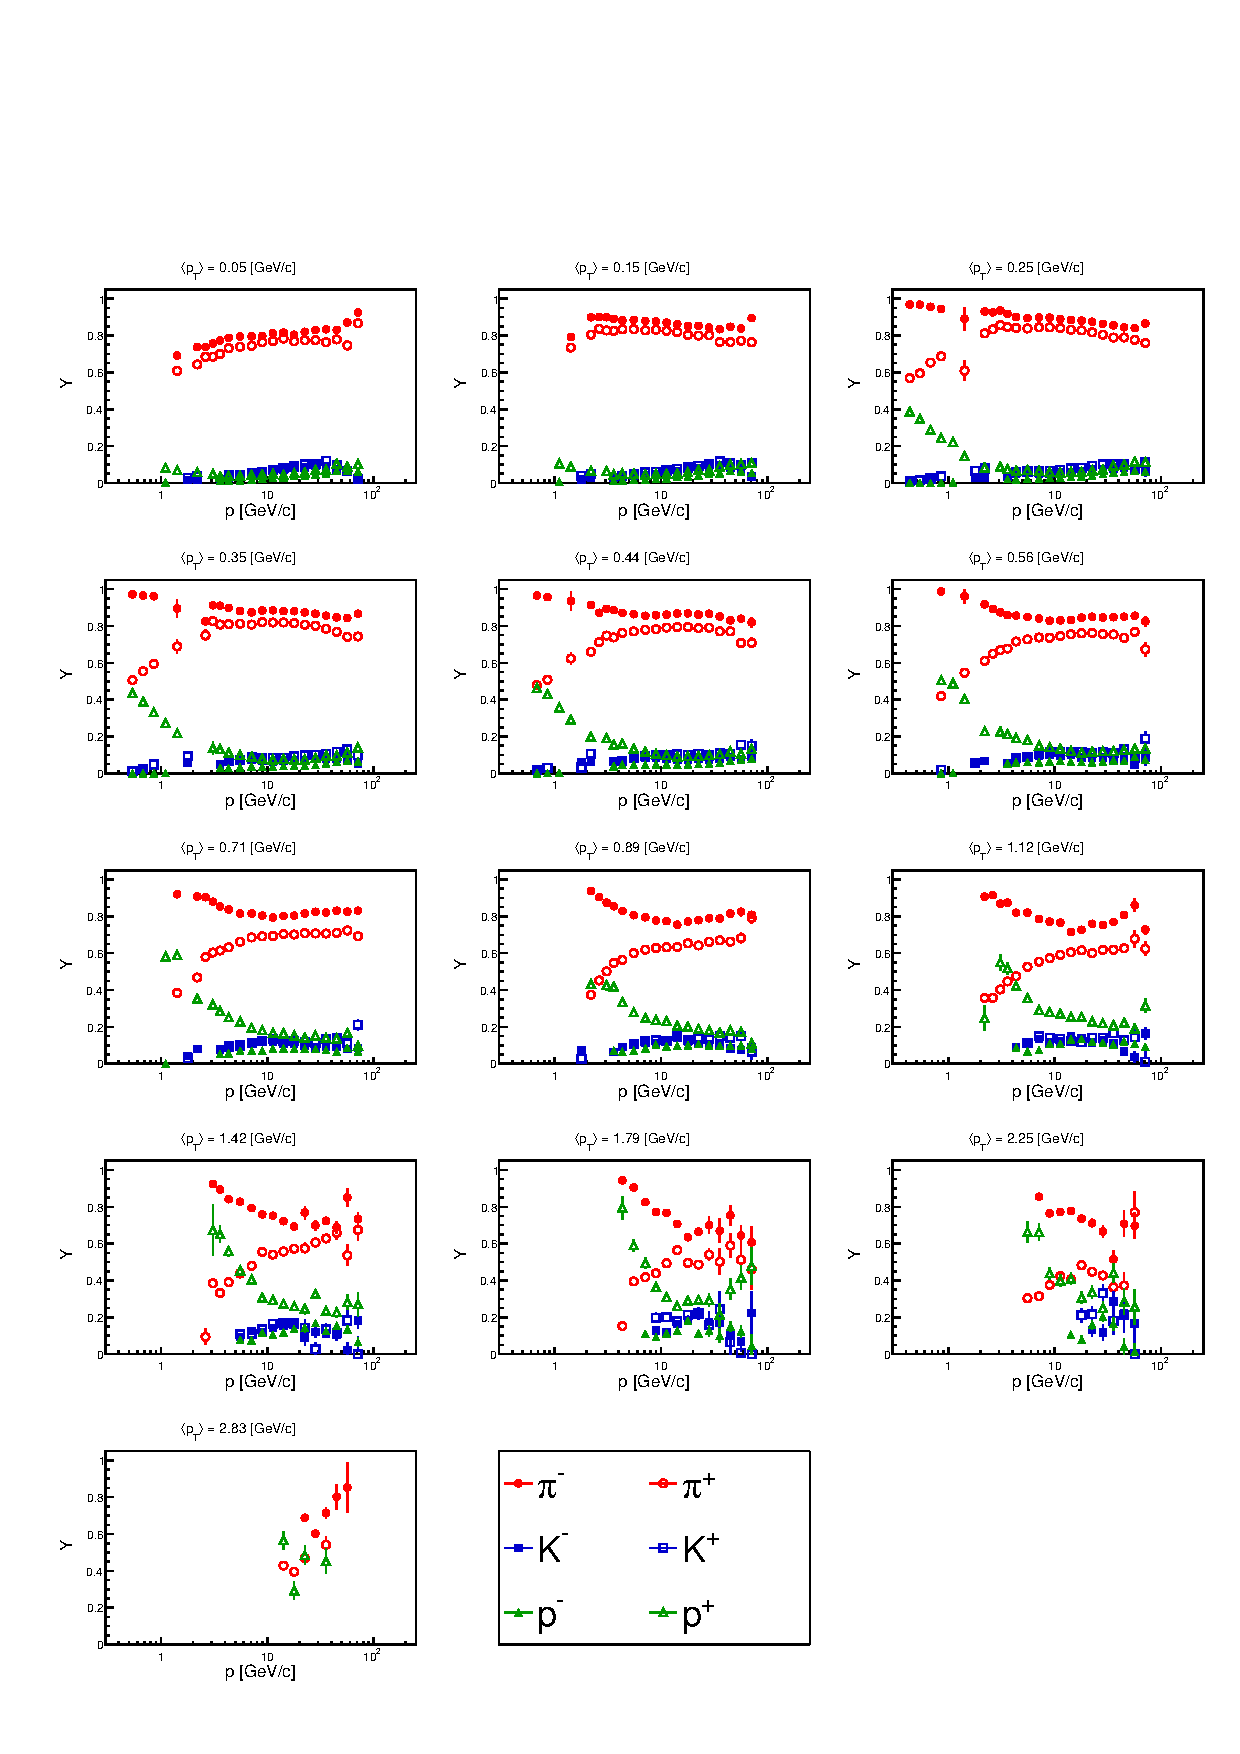
\includegraphics[clip, rviewport=0 0 1 1,width=1.00\textwidth]{dedx/fraction_pt_158_fl2_v1}
  \caption{Particle fractions obtained from the \dedx fit,
    after applying the cuts and corrections (see~\cref{sec:hadron:dedx:sde}),
    of the WST and 158 \GeVc data set, with target inserted. Markers with different
    colors show particle types and negatively (positively) charged particles are shown
    in full (open) symbols. The $\langle\pT\rangle$ is indicated on the top of each plot.}
  \label{fig:hadron:dedx:fit:final158w}
  \begin{center}
    Source: By the author. 
  \end{center}
\end{figure}

\begin{figure}
  \centering
  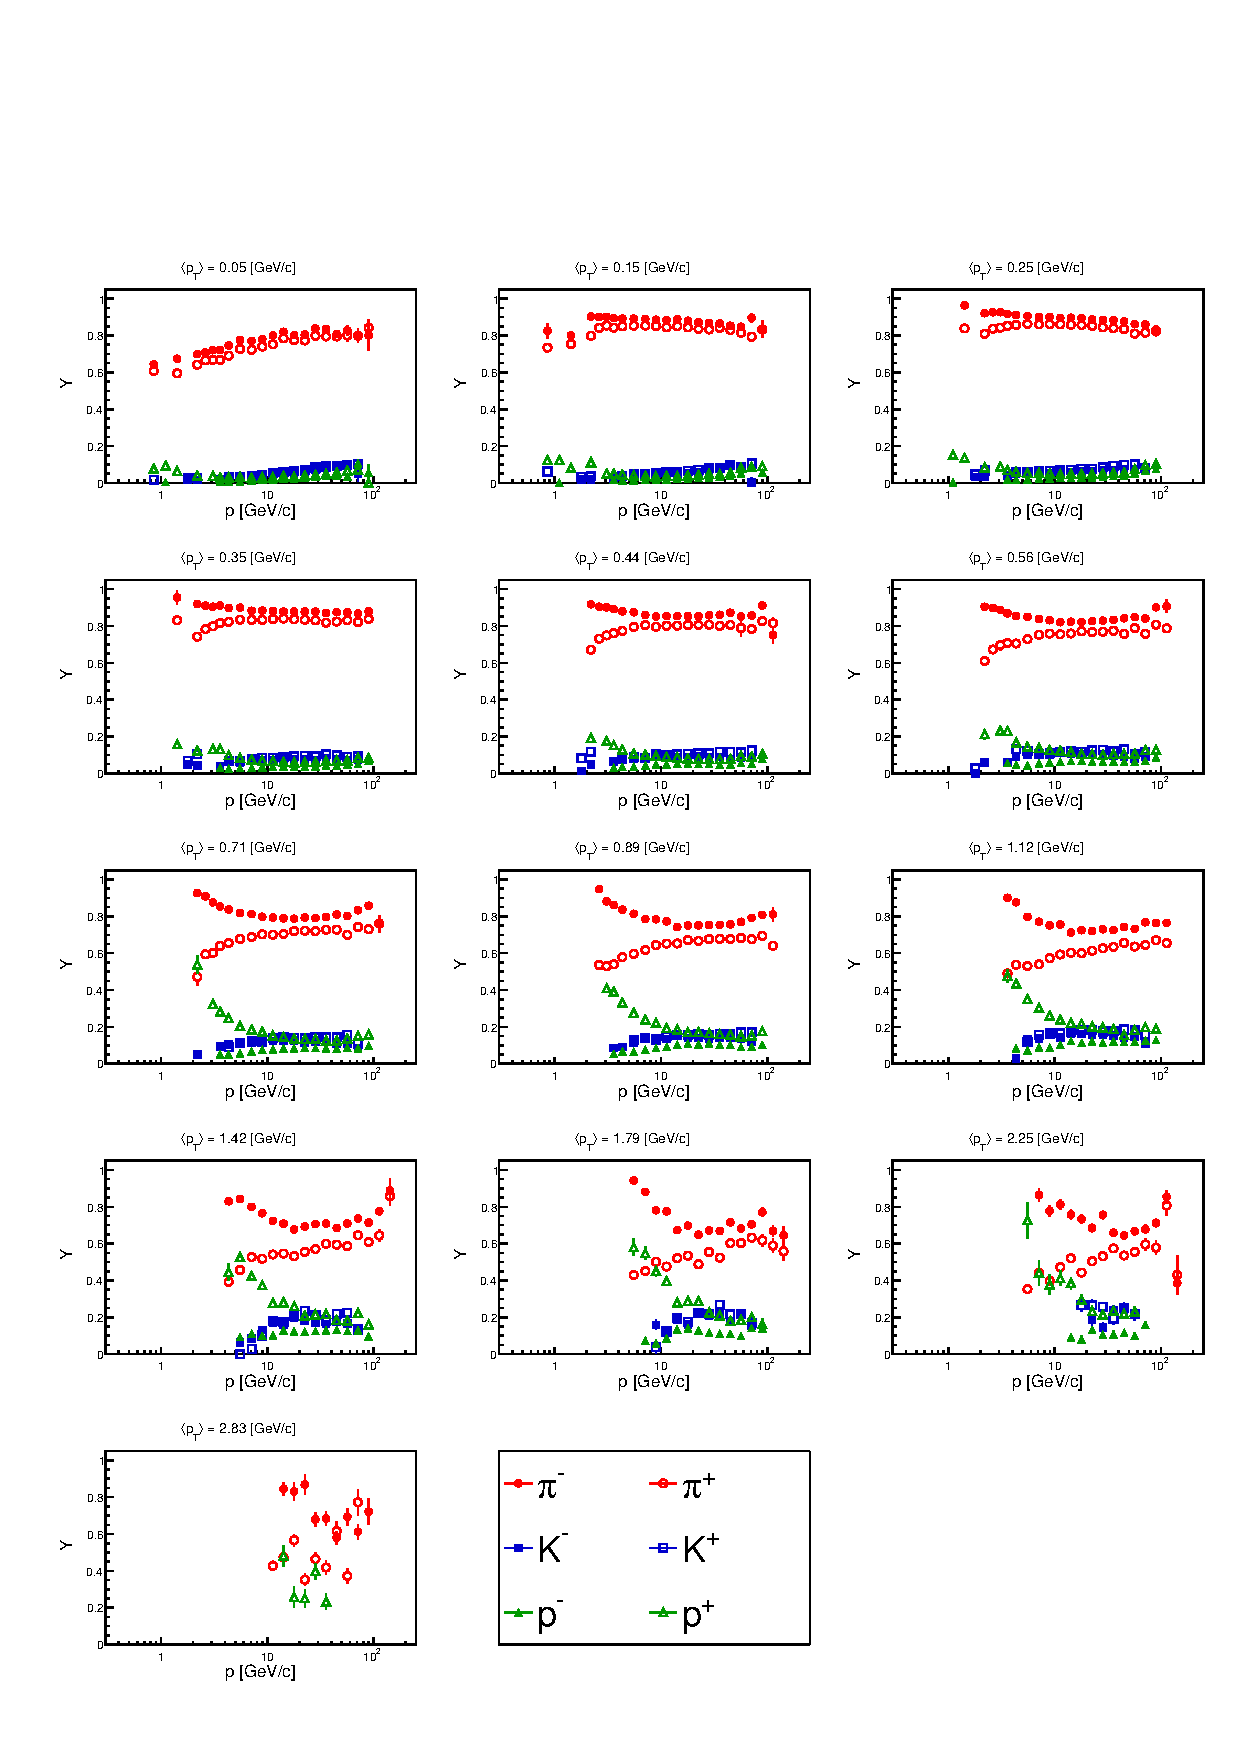
\includegraphics[clip, rviewport=0 0 1 1,width=1.00\textwidth]{dedx/fraction_pt_350_fl2_v0}
  \caption{Particle fractions obtained from the \dedx fit,
    after applying the cuts and corrections (see~\cref{sec:hadron:dedx:sde}),
    of the RST and 350 \GeVc data set, with target inserted. Markers with different
    colors show particle types and negatively (positively) charged particles are shown
    in full (open) symbols. The $\langle\pT\rangle$ is indicated on the top of each plot.}
  \label{fig:hadron:dedx:fit:final350r}
  \begin{center}
    Source: By the author. 
  \end{center}
\end{figure}

\begin{figure}
  \centering
  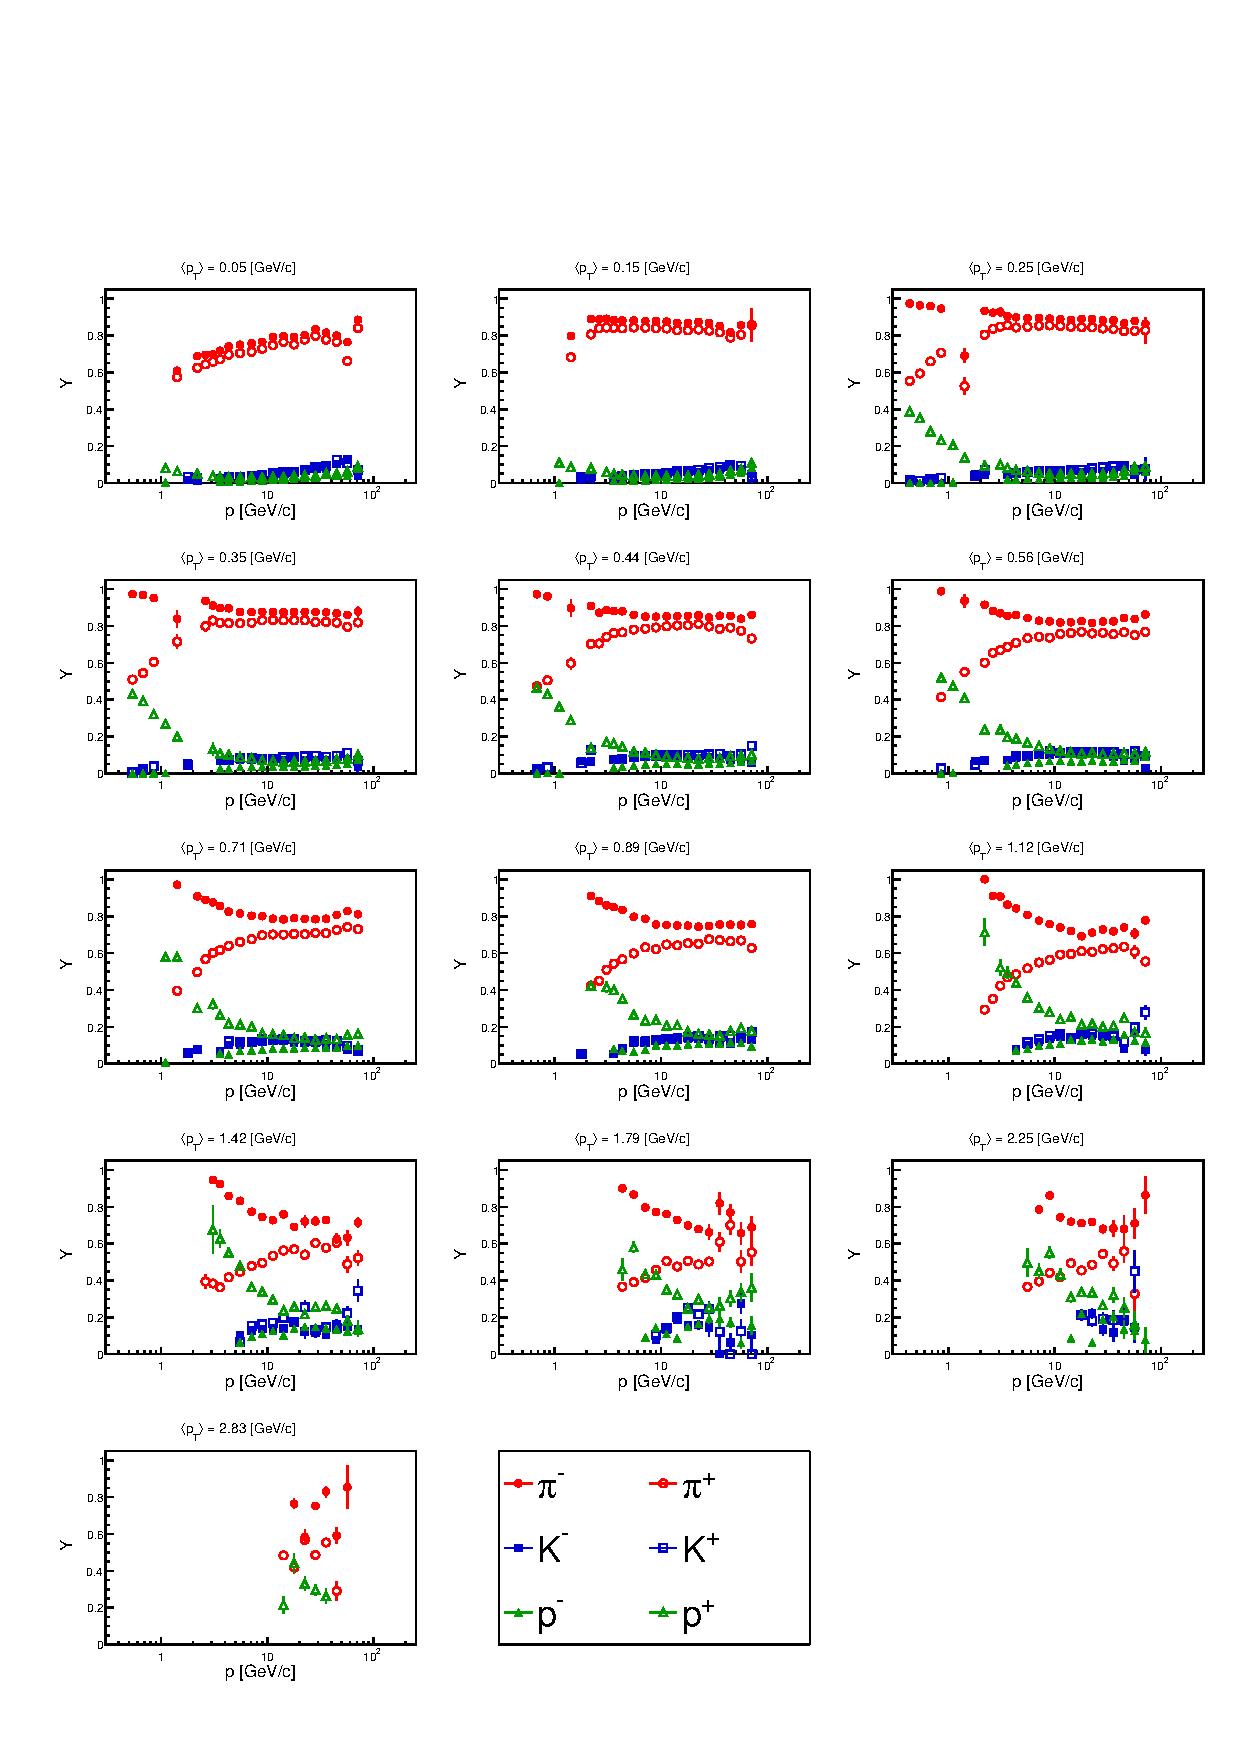
\includegraphics[clip, rviewport=0 0 1 1,width=1.00\textwidth]{dedx/fraction_pt_350_fl2_v1}
  \caption{Particle fractions obtained from the \dedx fit,
    after applying the cuts and corrections (see~\cref{sec:hadron:dedx:sde}),
    of the WST and 350 \GeVc data set, with target inserted. Markers with different
    colors show particle types and negatively (positively) charged particles are shown
    in full (open) symbols. The $\langle\pT\rangle$ is indicated on the top of each plot.}
  \label{fig:hadron:dedx:fit:final350w}
  \begin{center}
    Source: By the author. 
  \end{center}
\end{figure}

%%%%%%%%%% FRACTION OUT%%%%%%%%%%%%%%
\begin{figure}
  \centering
  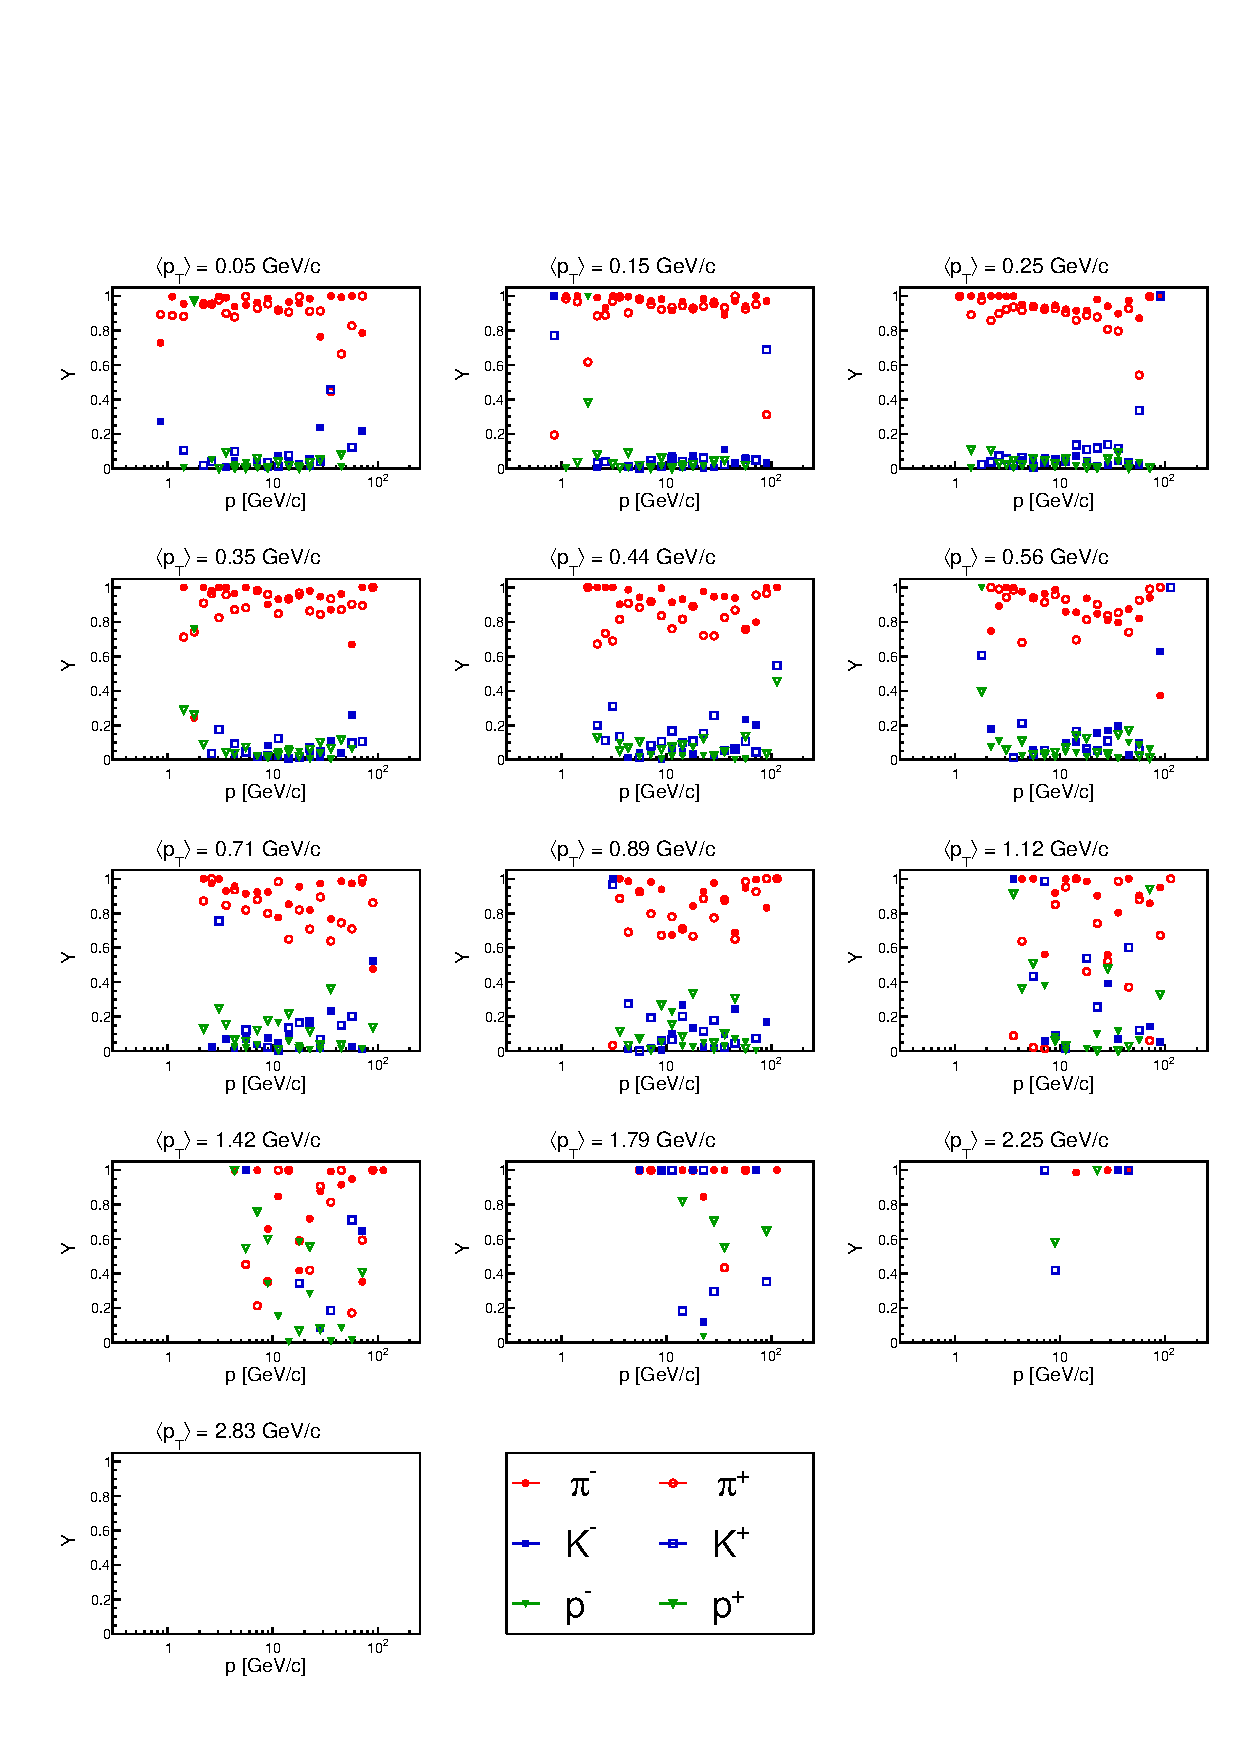
\includegraphics[clip, rviewport=0 0 1 1,width=1.00\textwidth]{dedx/fraction_out_pt_158_v0}
  \caption{Particle fractions obtained from the \dedx fit,
    after applying the cuts and corrections (see~\cref{sec:hadron:dedx:sde}),
    of the RST and 158 \GeVc data set, with target removed. Markers with different
    colors show particle types and negatively (positively) charged particles are shown
    in full (open) symbols. The $\langle\pT\rangle$ is indicated on the top of each plot.}
  \label{fig:hadron:dedx:fit:out158r}
  \begin{center}
    Source: By the author. 
  \end{center}
\end{figure}

\begin{figure}
  \centering
  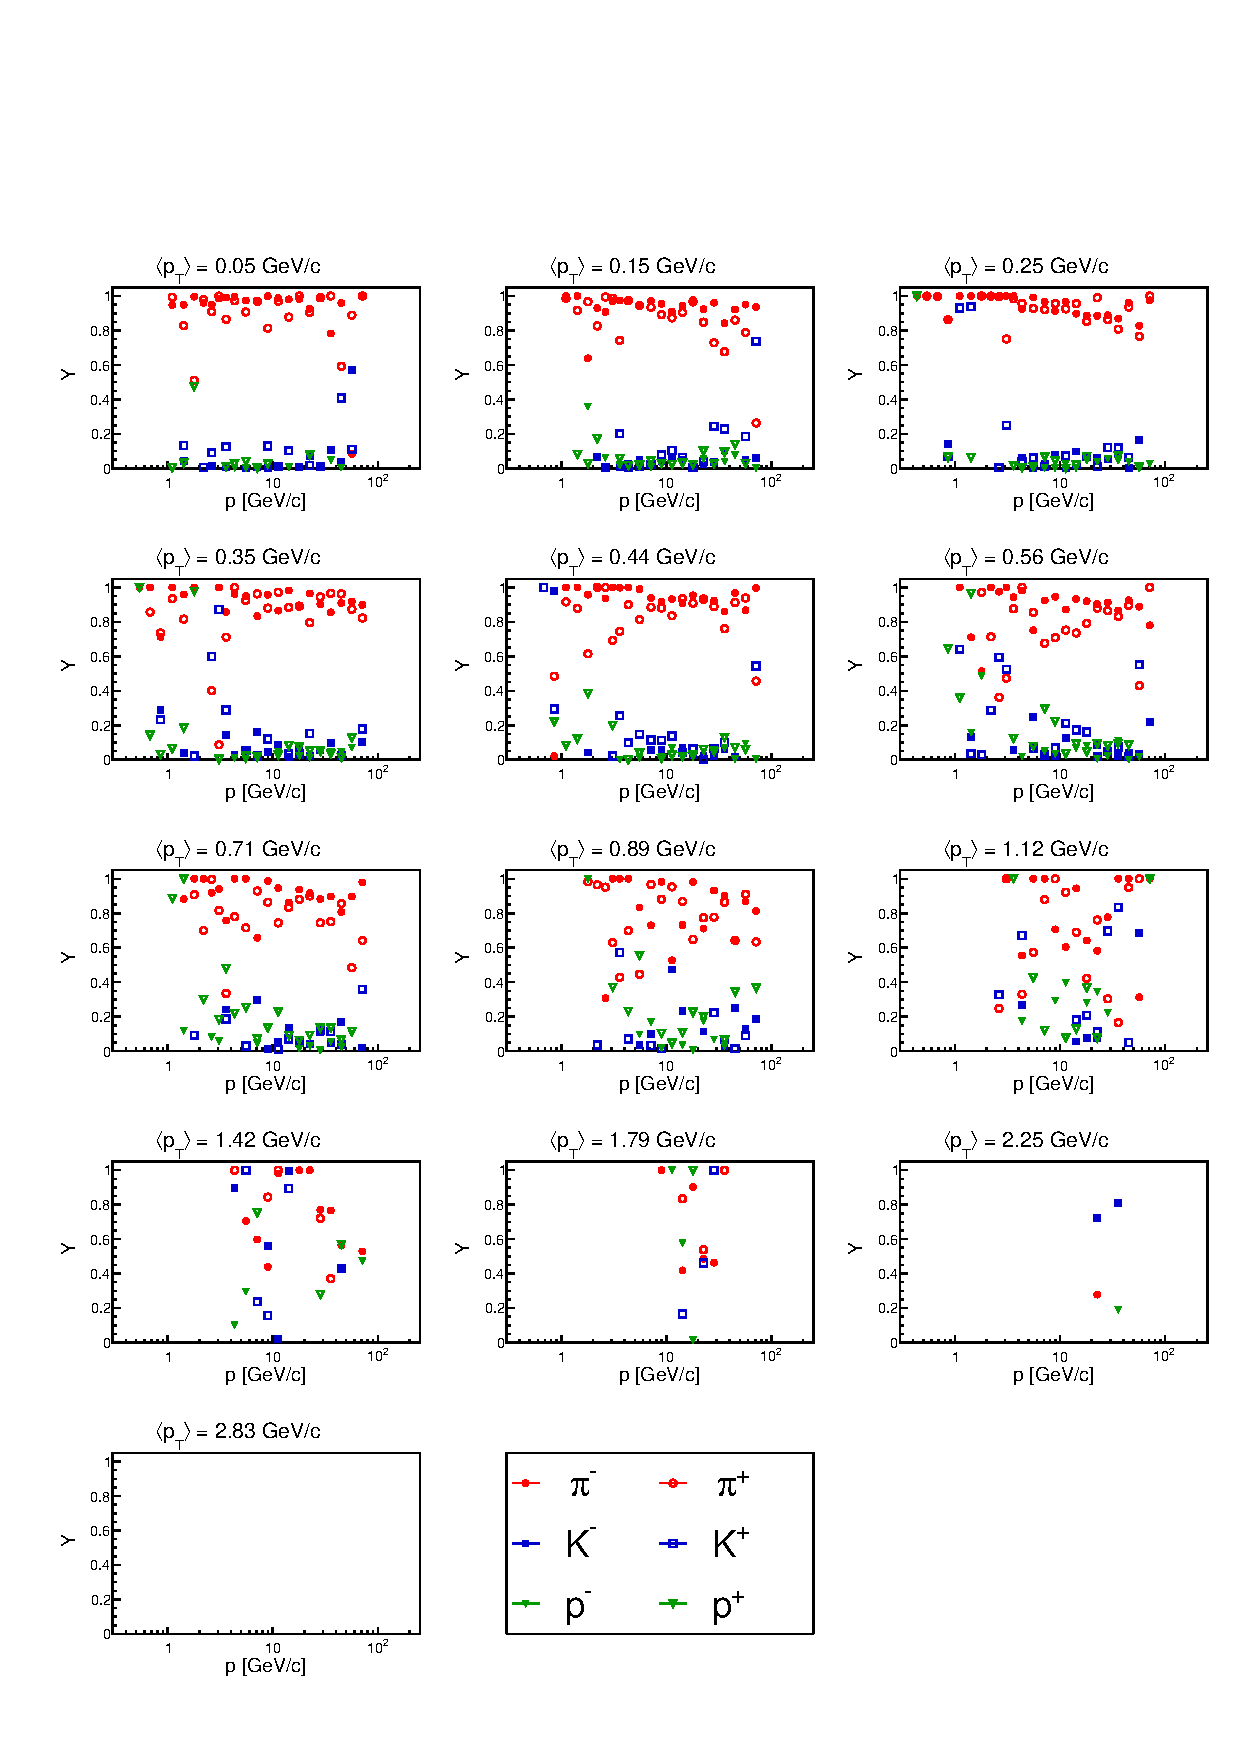
\includegraphics[clip, rviewport=0 0 1 1,width=1.00\textwidth]{dedx/fraction_out_pt_158_v1}
  \caption{Particle fractions obtained from the \dedx fit,
    after applying the cuts and corrections (see~\cref{sec:hadron:dedx:sde}),
    of the WST and 158 \GeVc data set, with target removed. Markers with different
    colors show particle types and negatively (positively) charged particles are shown
    in full (open) symbols. The $\langle\pT\rangle$ is indicated on the top of each plot.}
  \label{fig:hadron:dedx:fit:out158w}
  \begin{center}
    Source: By the author. 
  \end{center}
\end{figure}

\begin{figure}
  \centering
  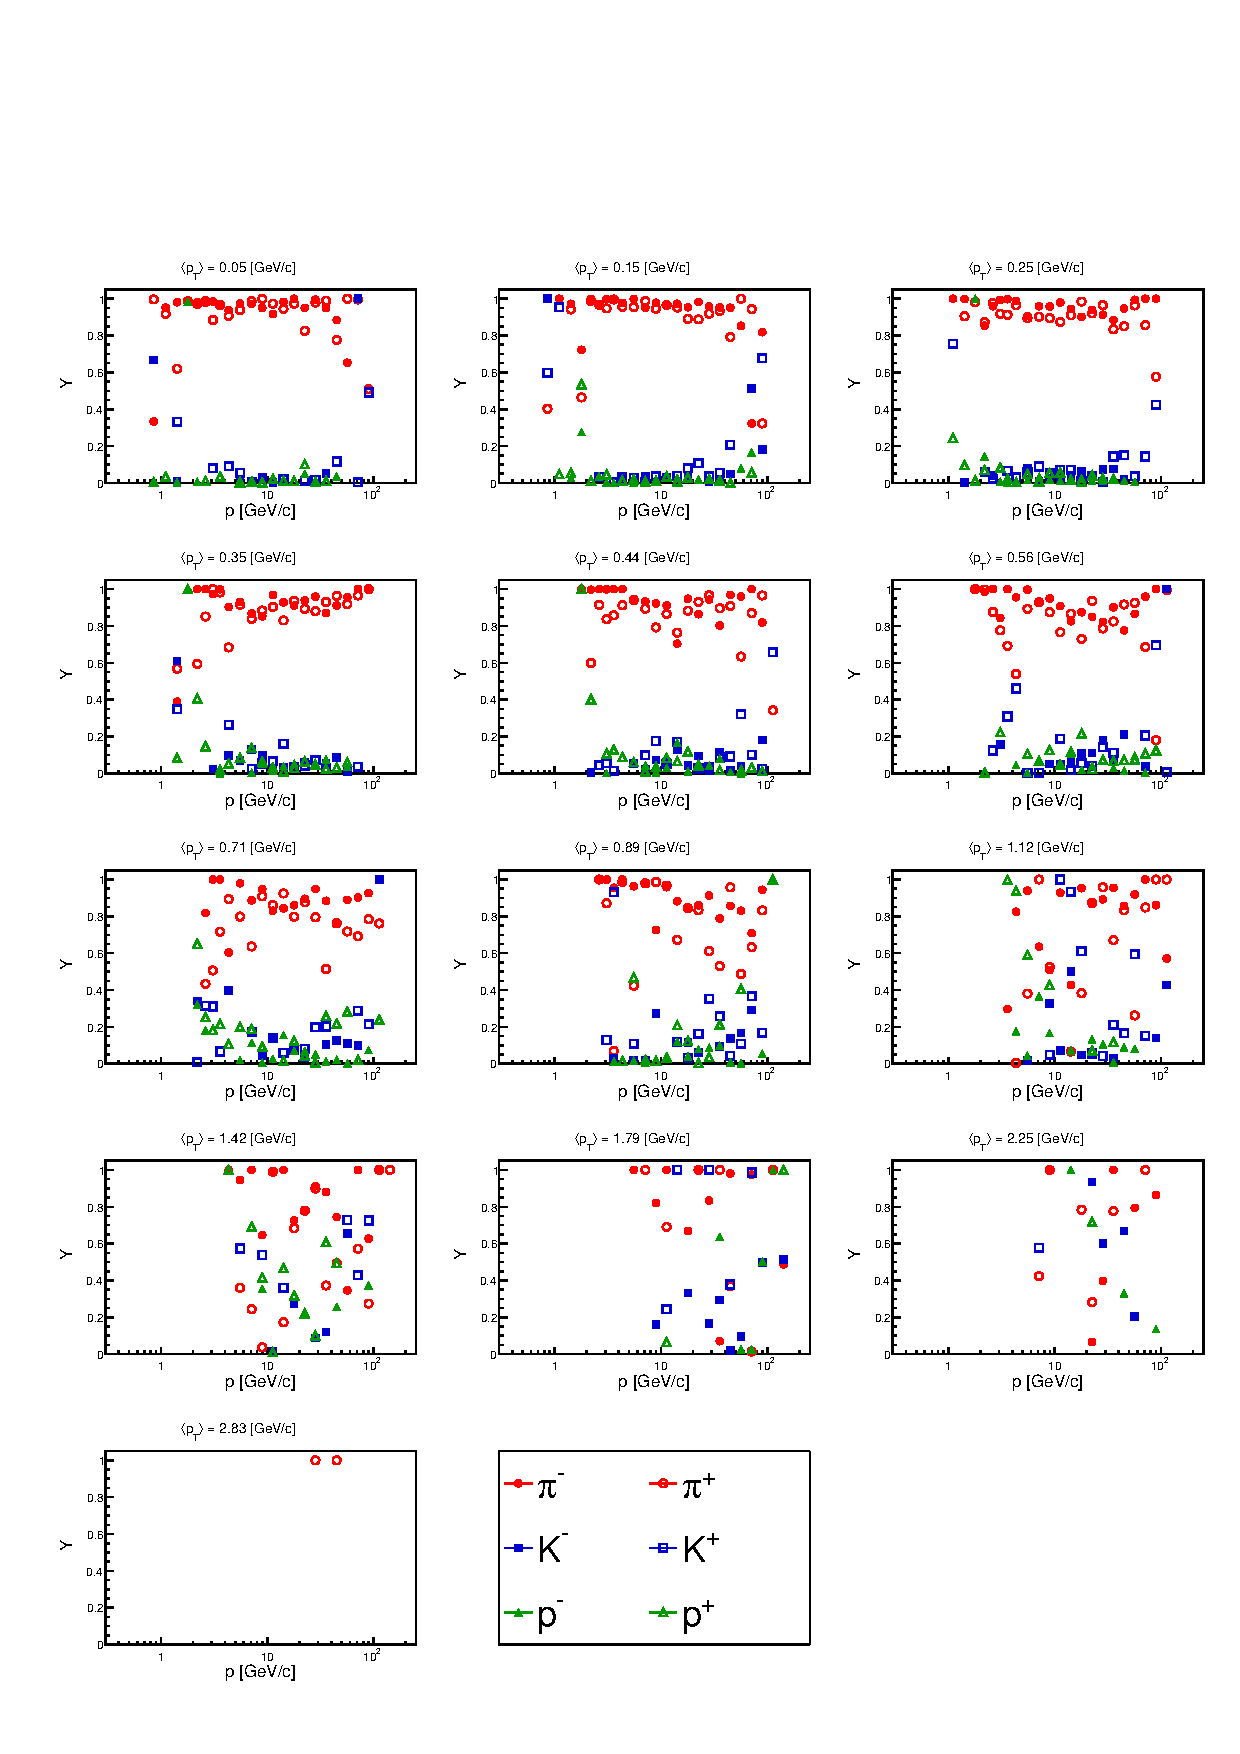
\includegraphics[clip, rviewport=0 0 1 1,width=1.00\textwidth]{dedx/fraction_out_pt_350_v0}
  \caption{Particle fractions obtained from the \dedx fit,
    after applying the cuts and corrections (see~\cref{sec:hadron:dedx:sde}),
    of the RST and 350 \GeVc data set, with target removed. Markers with different
    colors show particle types and negatively (positively) charged particles are shown
    in full (open) symbols. The $\langle\pT\rangle$ is indicated on the top of each plot.}
  \label{fig:hadron:dedx:fit:out350r}
  \begin{center}
    Source: By the author. 
  \end{center}
\end{figure}

\begin{figure}
  \centering
  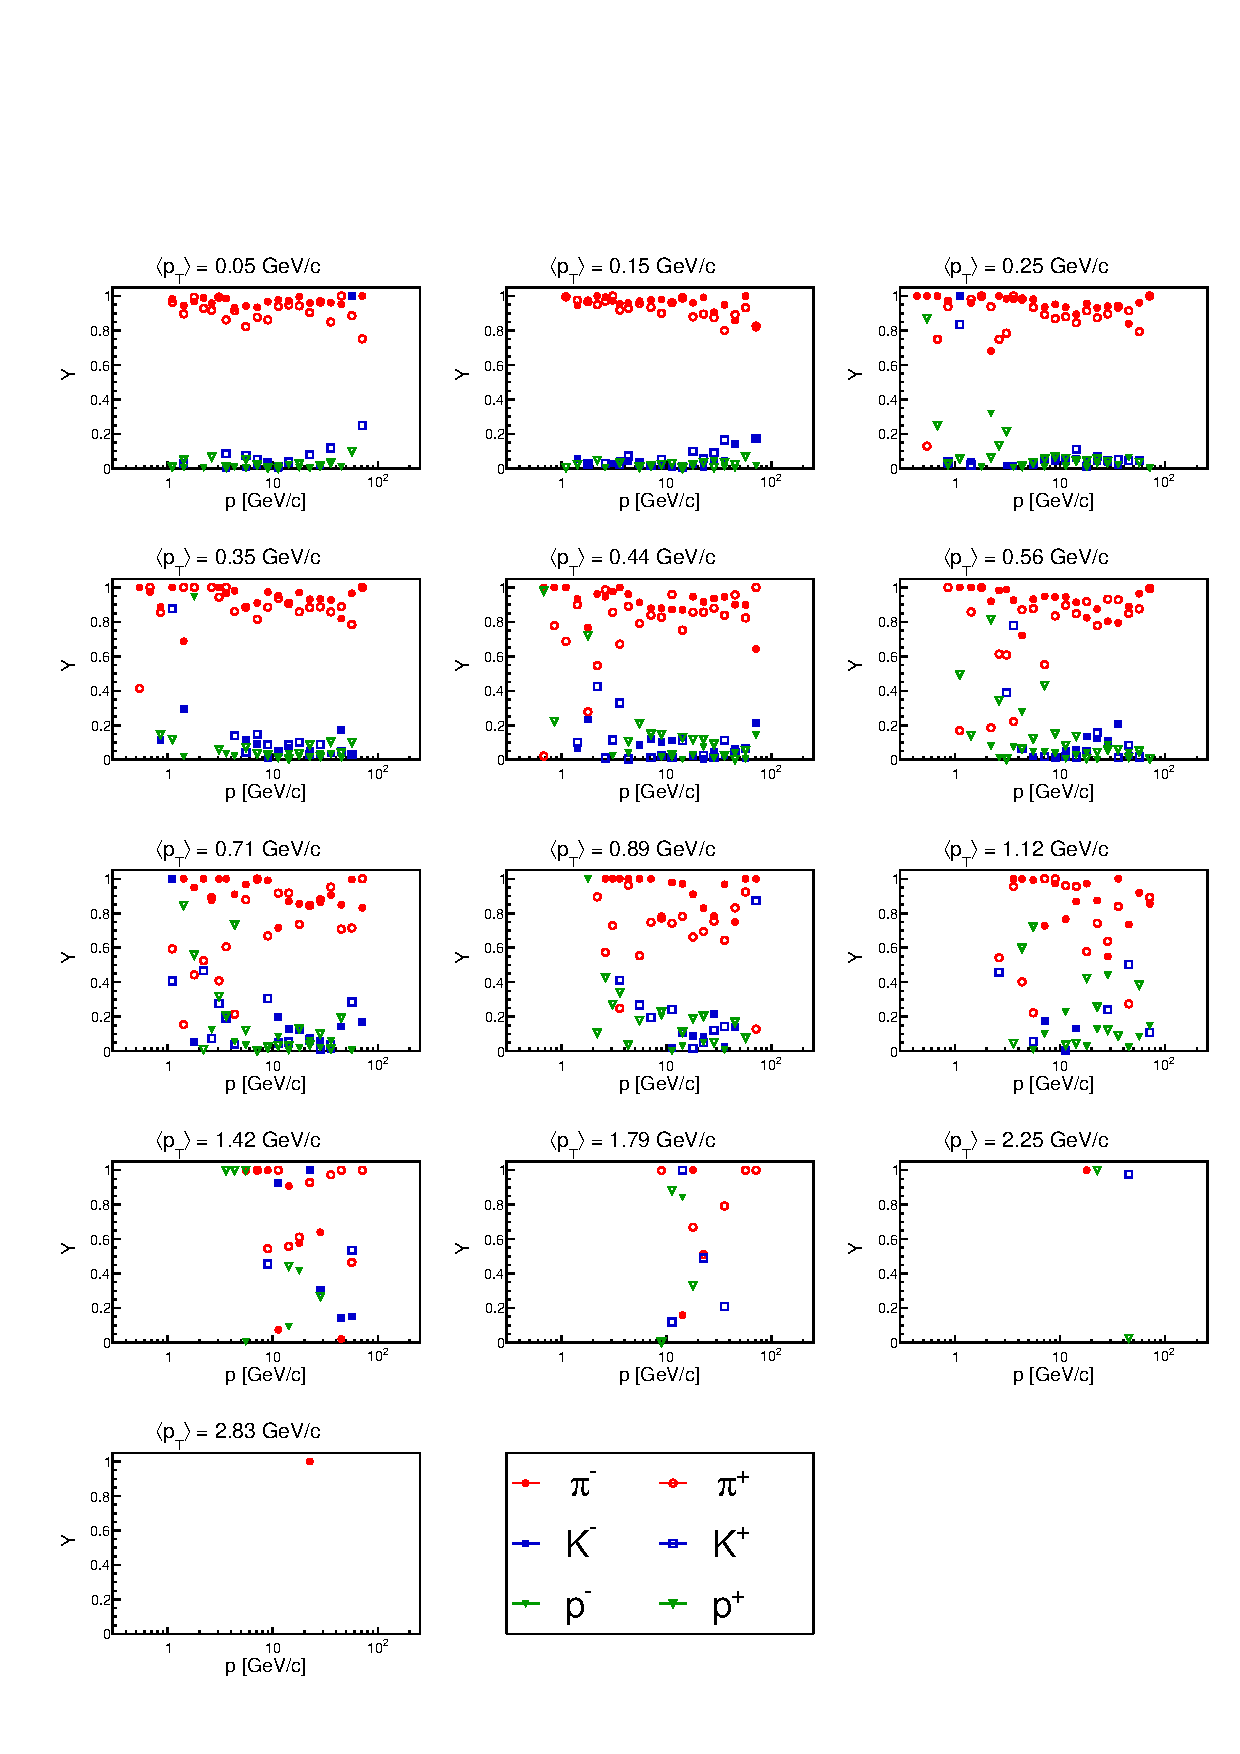
\includegraphics[clip, rviewport=0 0 1 1,width=1.00\textwidth]{dedx/fraction_out_pt_350_v1}
  \caption{Particle fractions obtained from the \dedx fit,
    after applying the cuts and corrections (see~\cref{sec:hadron:dedx:sde}),
    of the WST and 350 \GeVc data set, with target removed. Markers with different
    colors show particle types and negatively (positively) charged particles are shown
    in full (open) symbols. The $\langle\pT\rangle$ is indicated on the top of each plot.}
  \label{fig:hadron:dedx:fit:out350w}
  \begin{center}
    Source: By the author. 
  \end{center}
\end{figure}

%%%%%%%%%%% DECAY DIST CUT %%%%%%%%%%%%%%%%%%
\begin{figure}
  \centering

  \begin{overpic}[clip, rviewport=0 0 1 1,width=0.99\textwidth]{vzero/cut_dist_Data350}
    \put(28,20){(a)}
    \put(61,20){(b)}
    \put(95,20){(c)}
  \end{overpic}

  \caption{Optimization of the \decaydistmin for the 350 \GeVc data set.
    The \lamb case is shown in (a), \antilamb in (b) and \kzeros in (c).
    Individual phase space bins are shown as black markers, the average over
    \pT bins is shown as red markers.}
  \label{fig:hadron:vzero:cuts:decaydist:350}
  \begin{center}
    Source: By the author. 
  \end{center}
\end{figure}


\clearpage

%%%%%%%%%%% DIST IN %%%%%%%%%%%%%%%%%%
\begin{figure}[!ht]
  \centering
  \begin{overpic}[clip, rviewport=0 0 1 1,width=0.32\textwidth]{vzero/mass_Data350_t0_ph1_h0_x1_y3}
    \put(14,86){(a) \lamb}
  \end{overpic}
  \begin{overpic}[clip, rviewport=0 0 1 1,width=0.32\textwidth]{vzero/mass_Data350_t0_ph1_h1_x1_y3}
    \put(14,86){(b) \antilamb}
  \end{overpic}
  \begin{overpic}[clip, rviewport=0 0 1 1,width=0.32\textwidth]{vzero/mass_Data350_t0_ph1_h2_x2_y4}
    \put(14,86){(c) \kzeros}
  \end{overpic}

  \vspace{0.5cm}
  
  \begin{overpic}[clip, rviewport=0 0 1 1,width=0.32\textwidth]{vzero/mass_Data350_t0_ph1_h0_x5_y0}
    \put(14,86){(d) \lamb}
  \end{overpic}
  \begin{overpic}[clip, rviewport=0 0 1 1,width=0.32\textwidth]{vzero/mass_Data350_t0_ph1_h1_x5_y0}
    \put(14,86){(e) \antilamb}
  \end{overpic}
  \begin{overpic}[clip, rviewport=0 0 1 1,width=0.32\textwidth]{vzero/mass_Data350_t0_ph1_h2_x5_y1}
    \put(14,86){(f) \kzeros}
  \end{overpic}

  \caption{Examples of the fitted \minv distributions for the 350 \GeVc data set with target inserted.
    Two phase space bins are shown for \lamb in (a) and (d),
    for \antilamb in (b) and (e) and for \kzeros in (c) and (f).
    The black markers show the measured \minv distributions. The colored curves show
    the results of the fit, being the signal in blue, the background in red and the total in gray.
    Additionally, in green and purple we show the contributions of the two separated templates.
    On the bottom of each plot we show the residual distributions, being $\Delta$ the difference
    between observed and fitted number of entries and $\sigma$ the uncertainties of the observed number.
    The $\langle\pp\rangle$ and $\langle\pT\rangle$ of the phase space bin are
    indicated on the top of each plot.}
  \label{fig:hadron:vzero:signal:dist:350:in}
  \begin{center}
    Source: By the author. 
  \end{center}
\end{figure}

%%%%%%%%%%% DIST OUT %%%%%%%%%%%%%%%%%%
\begin{figure}[!ht]
  \centering
  \begin{overpic}[clip, rviewport=0 0 1 1,width=0.32\textwidth]{vzero/mass_Data350_t1_ph0_h0_x3_y0}
    \put(14,86){(a) \lamb}
  \end{overpic}
  \begin{overpic}[clip, rviewport=0 0 1 1,width=0.32\textwidth]{vzero/mass_Data350_t1_ph0_h1_x3_y0}
    \put(14,86){(b) \antilamb}
  \end{overpic}
  \begin{overpic}[clip, rviewport=0 0 1 1,width=0.32\textwidth]{vzero/mass_Data350_t1_ph0_h2_x3_y0}
    \put(14,86){(c) \kzeros}
  \end{overpic}

  \caption{Examples of the fitted \minv distributions for the 350 \GeVc data set with target removed.
    One \pp bin is shown for \lamb in (a), for \antilamb in (b) and for \kzeros in (c).
    The black markers show the measured \minv distributions. The colored curves show
    the results of the fit, being the signal in blue, the background in red and the total in gray.
    On the bottom of each plot we show the residual distributions, being $\Delta$ the difference
    between observed and fitted number of entries and $\sigma$ the uncertainties of the observed number.
    The $\langle\pp\rangle$ of the phase space bin is indicated on the top of each plot.}
  \label{fig:hadron:vzero:signal:dist:350:out}
  \begin{center}
    Source: By the author. 
  \end{center}
\end{figure}

\clearpage

%%%%%%%%%%% CHI SQ IN %%%%%%%%%%%%%%%%%%
\begin{figure}[!ht]
  \centering

  \begin{overpic}[clip, rviewport=0 0 1 1,width=0.99\textwidth]{vzero/chisq_Data350_t0_ph1}
    \put(6,20){(a)\lamb}
    \put(39.5,20){(b)\antilamb}
    \put(72.5,20){(c)\kzeros}
  \end{overpic}

  \vspace{0.5cm}

\begin{overpic}[clip, rviewport=0 0 1 1,width=0.99\textwidth]{vzero/chisq_Data350_t1_ph0}
    \put(6,20){(d)\lamb}
    \put(39.5,20){(e)\antilamb}
    \put(72.5,20){(f)\kzeros}
  \end{overpic}

  \caption{\redchisq of the \minv fit of the 350 \GeVc data set
    for the target inserted (upper plots) and removed (lower plots).
    The \lamb cases are shown in (a) and (d),
    the \antilamb in (b) and (e) and the \kzeros in (c) and (f).}
  \label{fig:hadron:vzero:signal:chi:350}
  \begin{center}
    Source: By the author. 
  \end{center}
\end{figure}



%%%%%%%%%%% EXTRACTED SIGNAL %%%%%%%%%%%%%%%%%%
\begin{figure}[!ht]
  \centering
  \begin{overpic}[clip, rviewport=0 0 1 1,width=0.99\textwidth]{vzero/signal_Data350_t0}
    \put(6,20){(a)\lamb}
    \put(39.5,20){(b)\antilamb}
    \put(72.5,20){(c)\kzeros}
  \end{overpic}

  \vspace{0.5cm}
  
  \begin{overpic}[clip, rviewport=0 0 1 1,width=0.99\textwidth]{vzero/signal_Data350_t1}
    \put(6,20){(d)\lamb}
    \put(39.5,20){(e)\antilamb}
    \put(72.5,20){(f)\kzeros}
  \end{overpic}

  \caption{Extracted signal $S$ for the 350 \GeVc data set
    with target inserted (upper plots) and removed (lower plots).
    The \lamb cases are shown in (a) and (d),
    the \antilamb in (b) and (e) and the \kzeros in (c) and (f).}
  \label{fig:hadron:vzero:signal:extracted:350}
  \begin{center}
    Source: By the author. 
  \end{center}
\end{figure}

\clearpage


%%%%%%%%%% BETA %%%%%%%%%%%%%%%%
\begin{figure}[!ht]
  \centering

  \begin{overpic}[clip, rviewport=0 0.143 1 1,width=0.45\textwidth]{dedx/fac_350_All_beta_c0_p1}
    \put(20,53){(a) $\pi^+$}
  \end{overpic}
  \begin{overpic}[clip, rviewport=0 0.143 1 1,width=0.45\textwidth]{dedx/fac_350_All_beta_c1_p1}
    \put(20,53){(b) $\pi^-$}
  \end{overpic}

  \begin{overpic}[clip, rviewport=0 0.143 1 1,width=0.45\textwidth]{dedx/fac_350_All_beta_c0_p2}
    \put(20,53){(c) K$^+$}
  \end{overpic}
  \begin{overpic}[clip, rviewport=0 0.143 1 1,width=0.45\textwidth]{dedx/fac_350_All_beta_c1_p2}
    \put(20,53){(d) K$^-$}
  \end{overpic}
  
  \begin{overpic}[clip, rviewport=0 0 1 1,width=0.45\textwidth]{dedx/fac_350_All_beta_c0_p3}
    \put(20,63){(e) p$^+$}
  \end{overpic}
  \begin{overpic}[clip, rviewport=0 0 1 1,width=0.45\textwidth]{dedx/fac_350_All_beta_c1_p3}
    \put(20,63){(f) p$^-$}
  \end{overpic}
    
  \caption{$\beta$ correction factor for the charged hadron analysis
    and for the 350 \GeVc data set. The $\pi^+$ case is shown in (a),
    $\pi^-$ in (b), K$^+$ in (c), K$^-$ in (d), p$^+$ in (e) and p$^-$ in (f).}
  \label{fig:hadron:correction:beta:dedx350}
  \begin{center}
    Source: By the author. 
  \end{center}
\end{figure}


%%%%%%%%%%% BETA V0 %%%%%%%%%%%%%%%%%%
\begin{figure}[!ht]
  \centering

  \begin{overpic}[clip, rviewport=0 0 1 1,width=0.99\textwidth]{vzero/beta350}
    \put(0,22){(a)}
    \put(33,22){(b)}
    \put(67,22){(c)}
  \end{overpic}

  \caption{$\beta$ correction factor for the \vzero analysis
    and for the 350 \GeVc data set. The \lamb case is shown in (a),
    \antilamb in (b) and \kzeros in (c).}
  \label{fig:hadron:correction:beta:vzero350}
  \begin{center}
    Source: By the author. 
  \end{center}
\end{figure}

\clearpage

%%%%%%%%%% SPEC PT ALL DEDX %%%%%%%%%%%%%%
\begin{figure}[!ht]
  \centering

  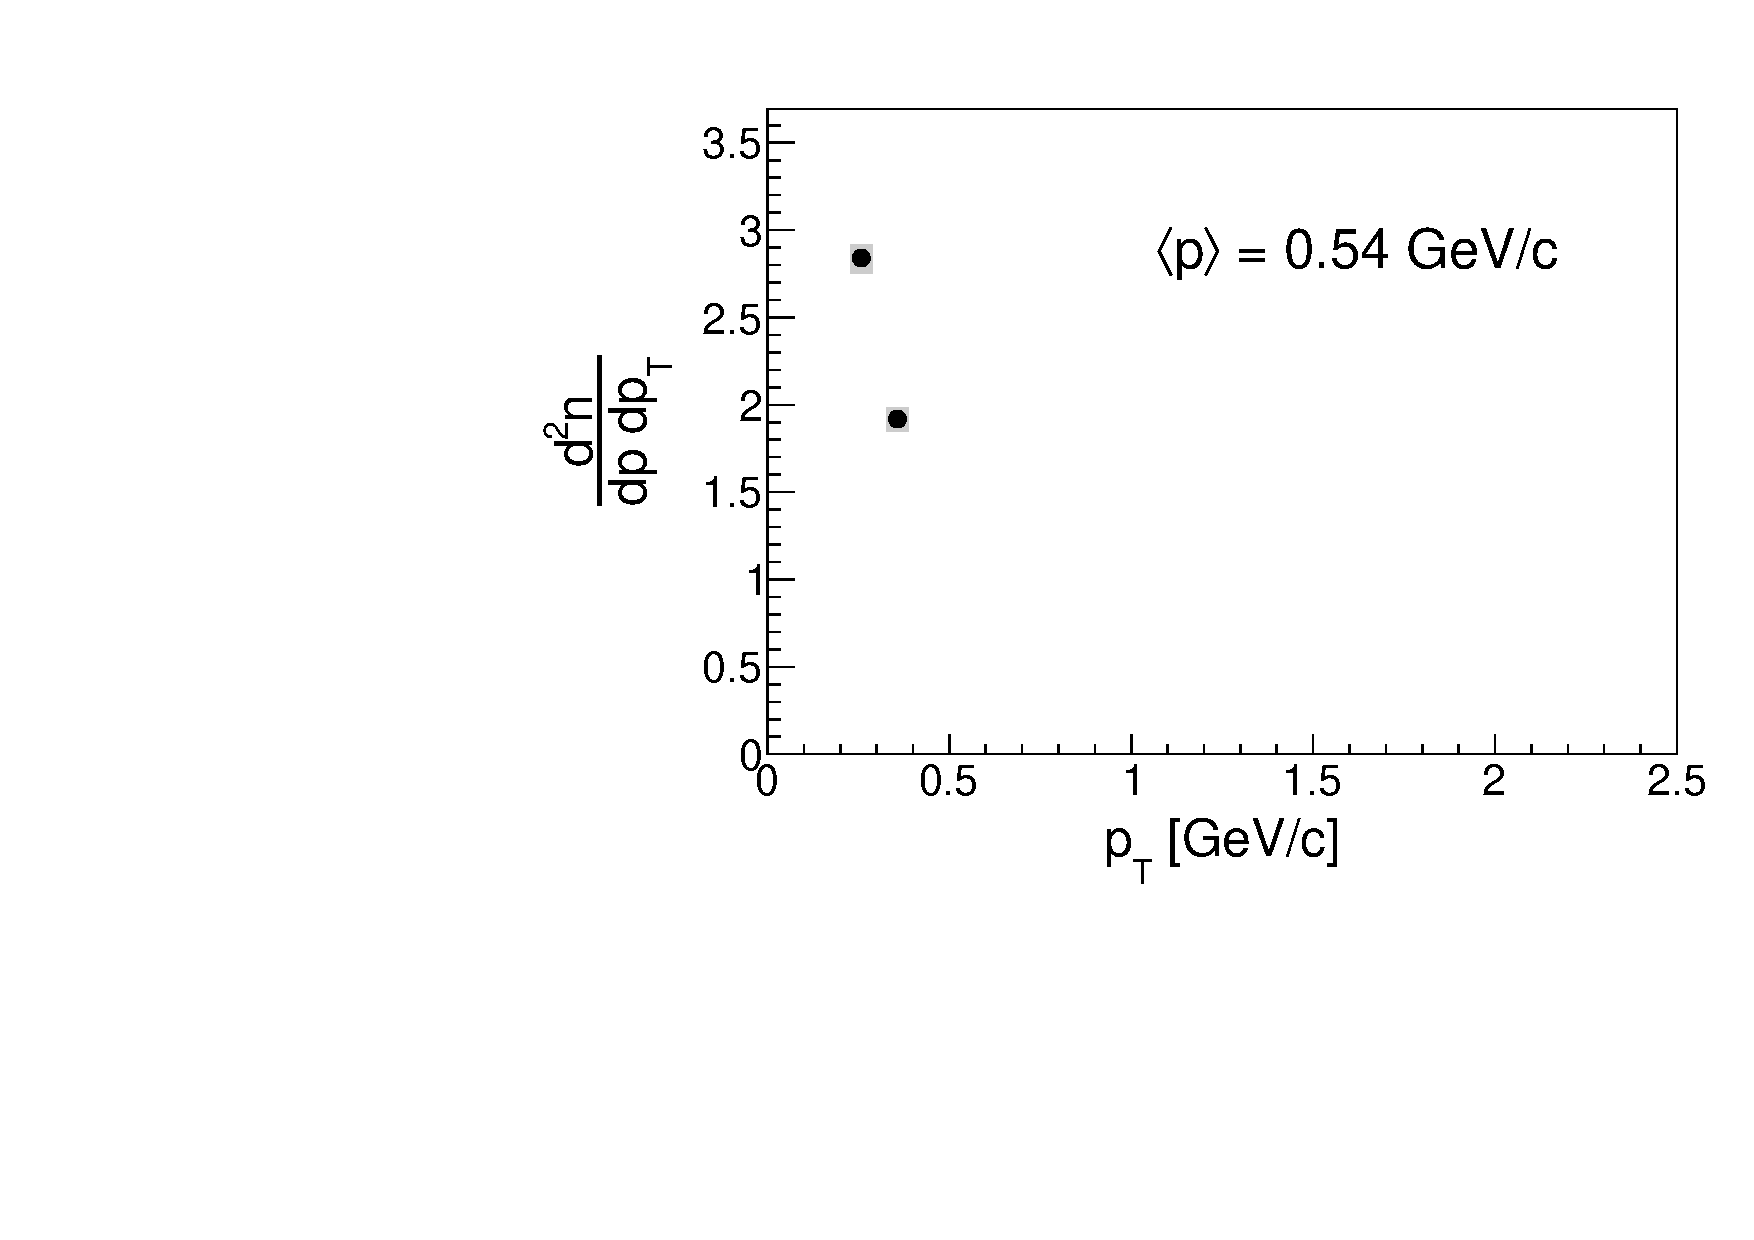
\includegraphics[clip, rviewport=0 0 1 1,width=0.24\textwidth]{spec/spec_pt_158_c0_p1_x7}
  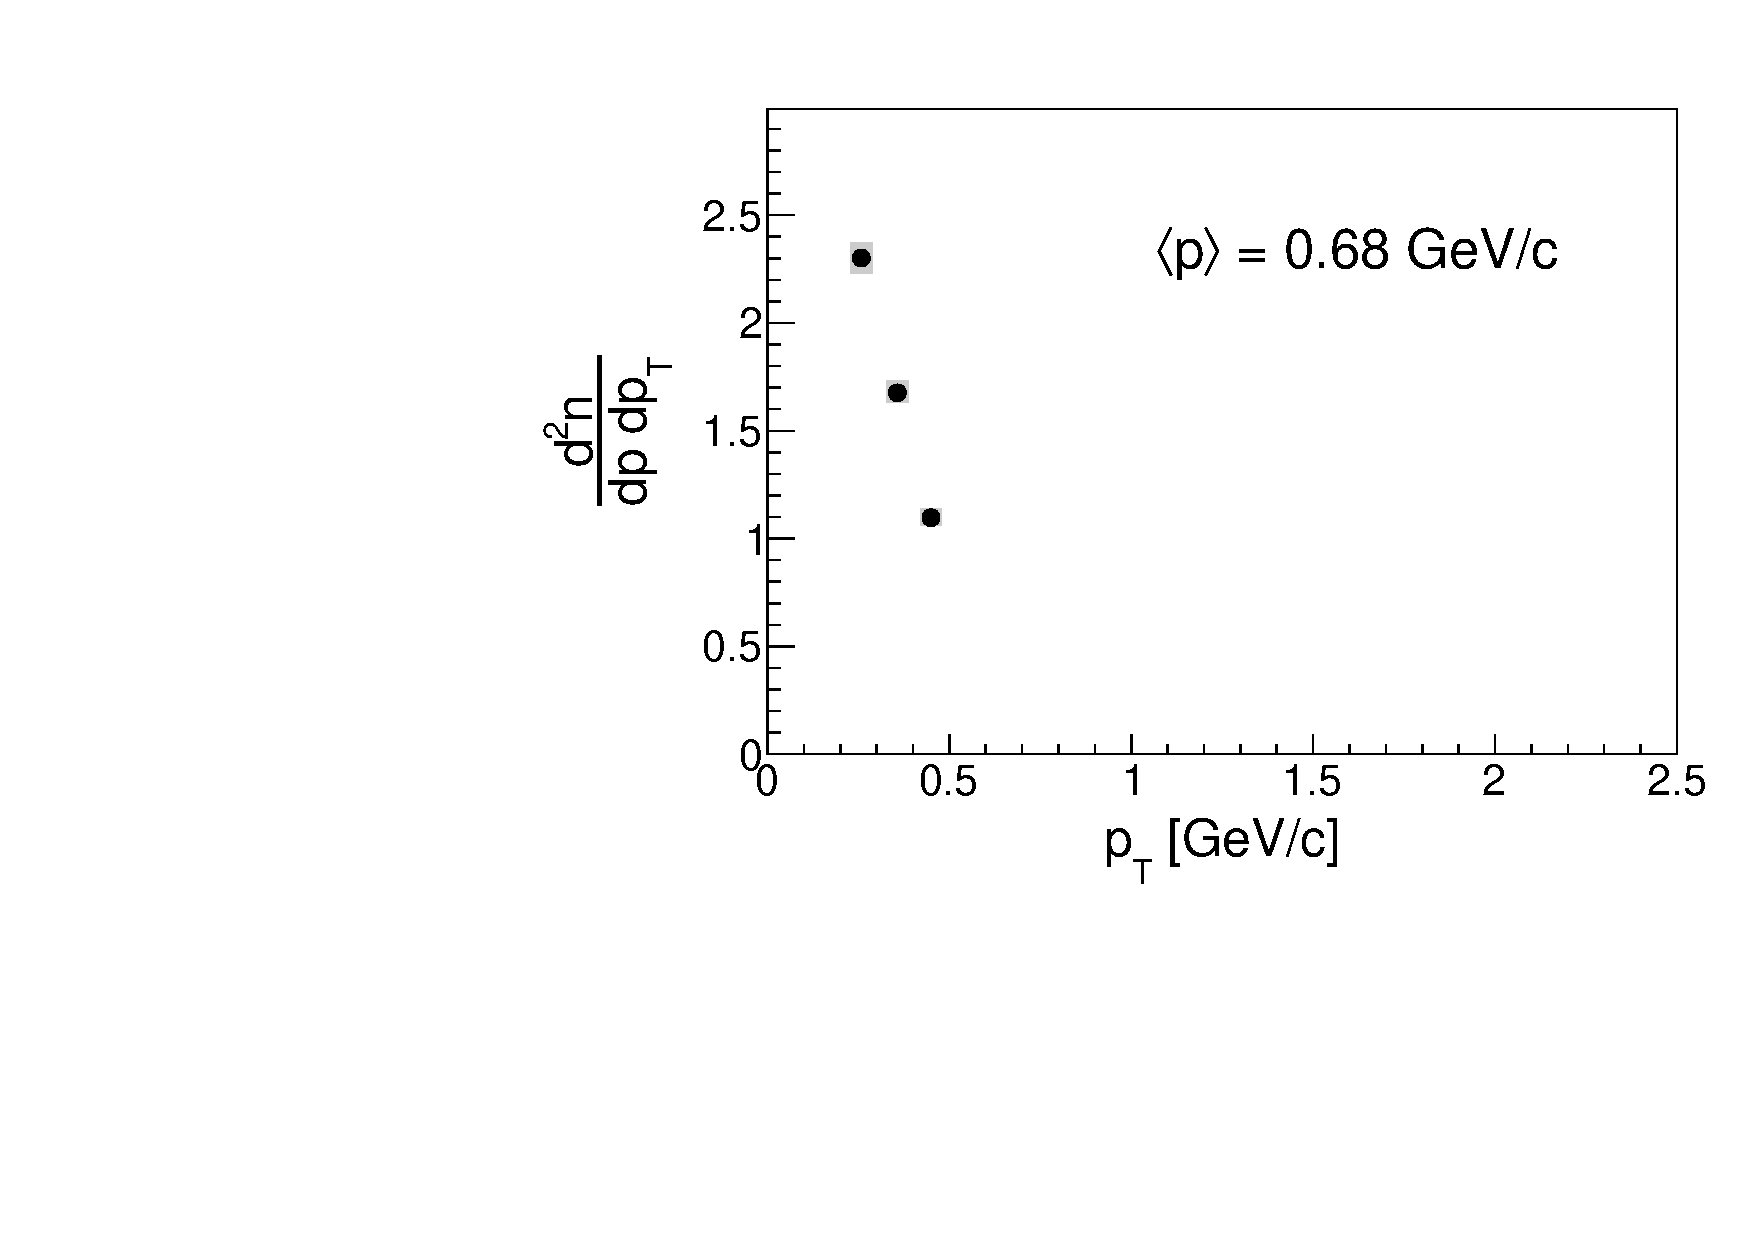
\includegraphics[clip, rviewport=0 0 1 1,width=0.24\textwidth]{spec/spec_pt_158_c0_p1_x8}
  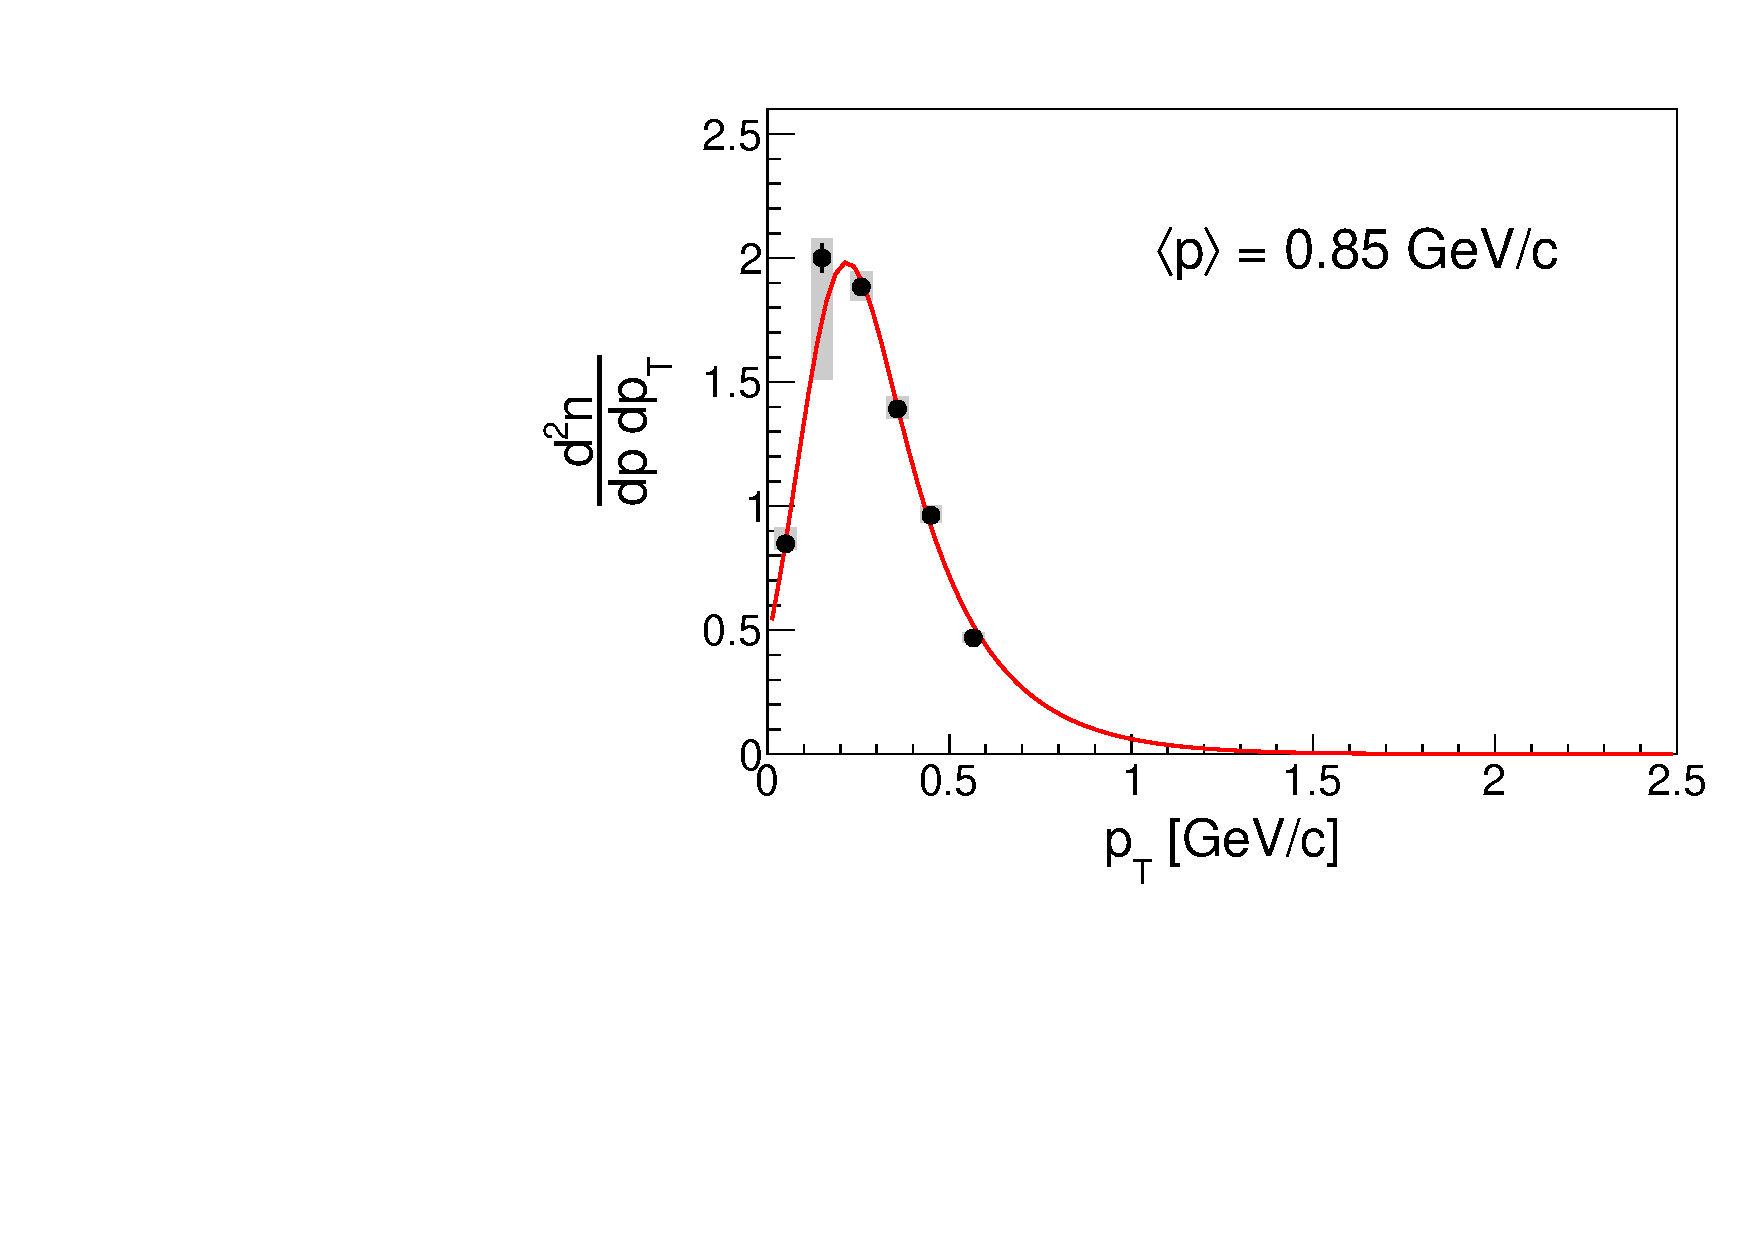
\includegraphics[clip, rviewport=0 0 1 1,width=0.24\textwidth]{spec/spec_pt_158_c0_p1_x9}
  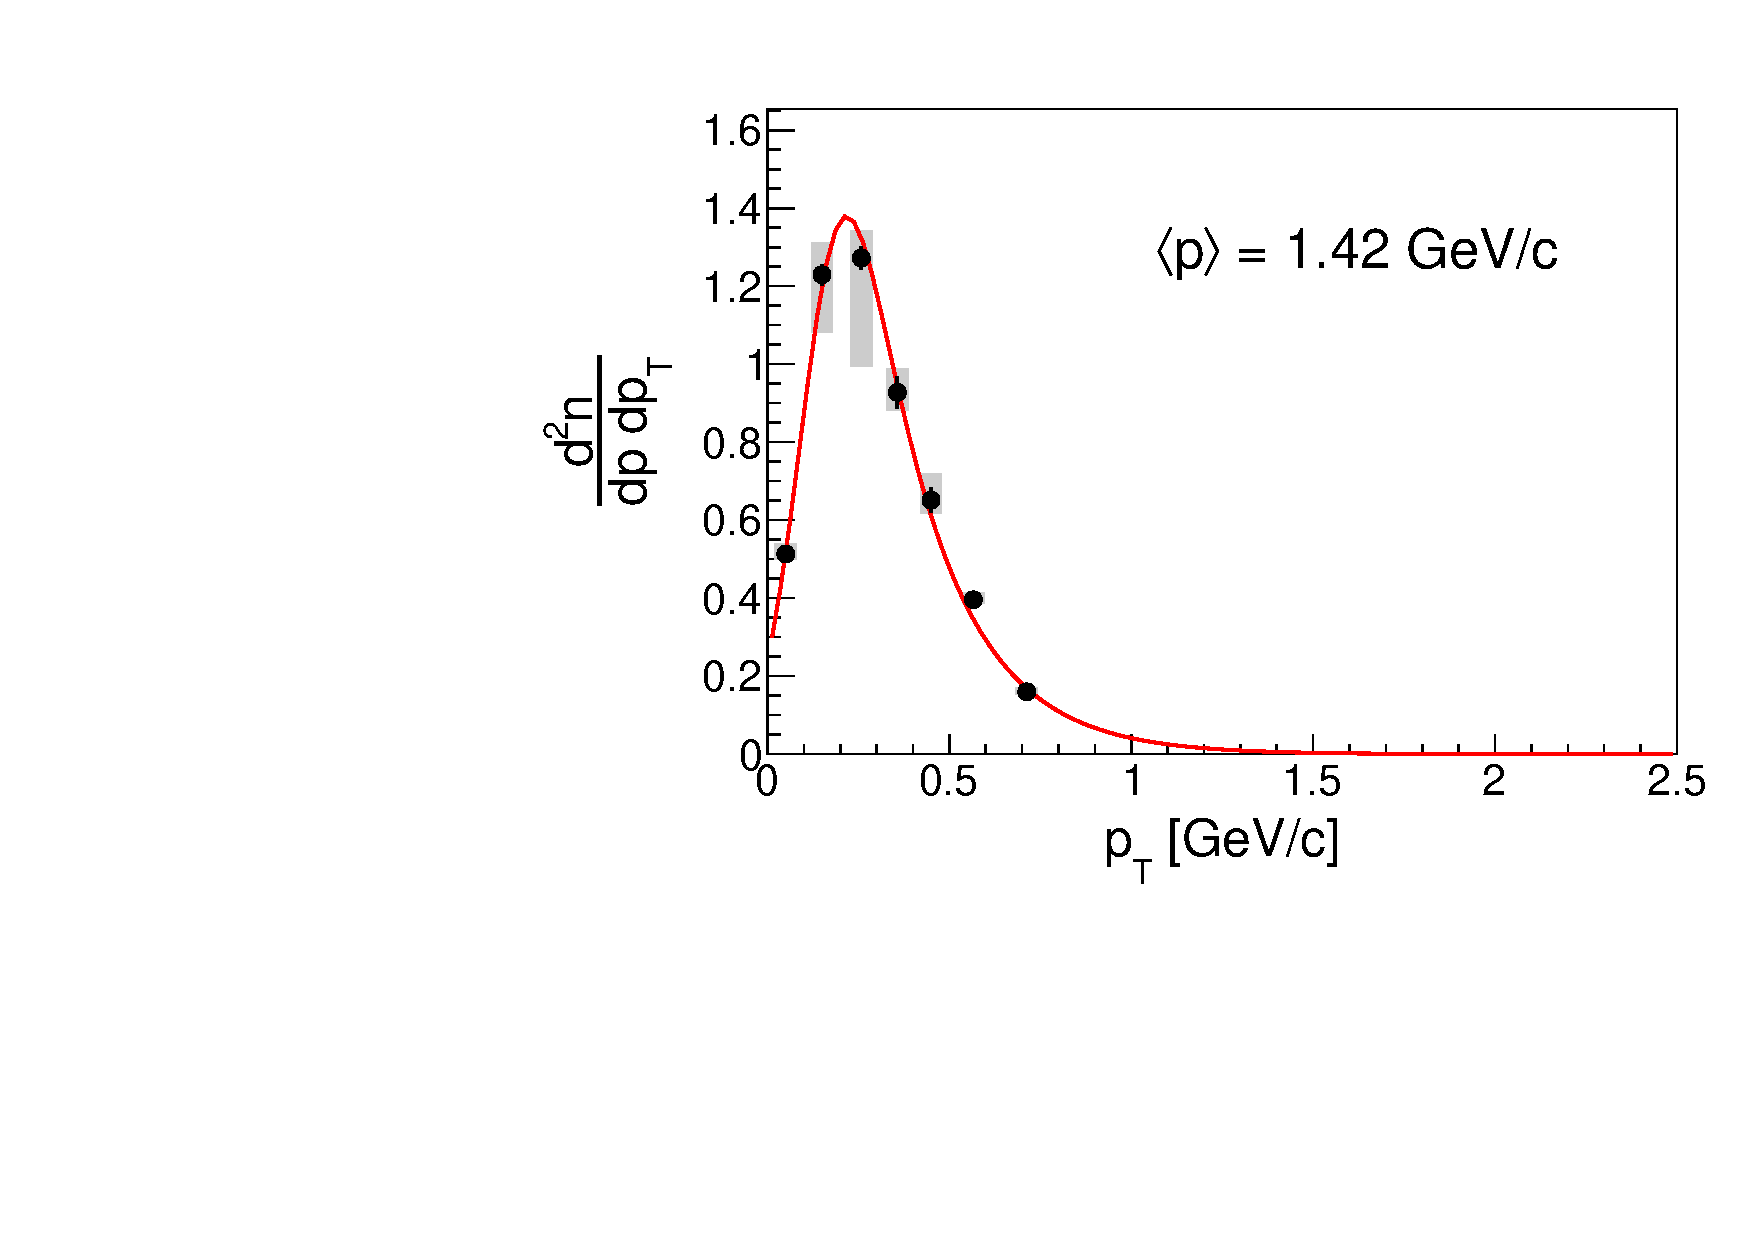
\includegraphics[clip, rviewport=0 0 1 1,width=0.24\textwidth]{spec/spec_pt_158_c0_p1_x11}

  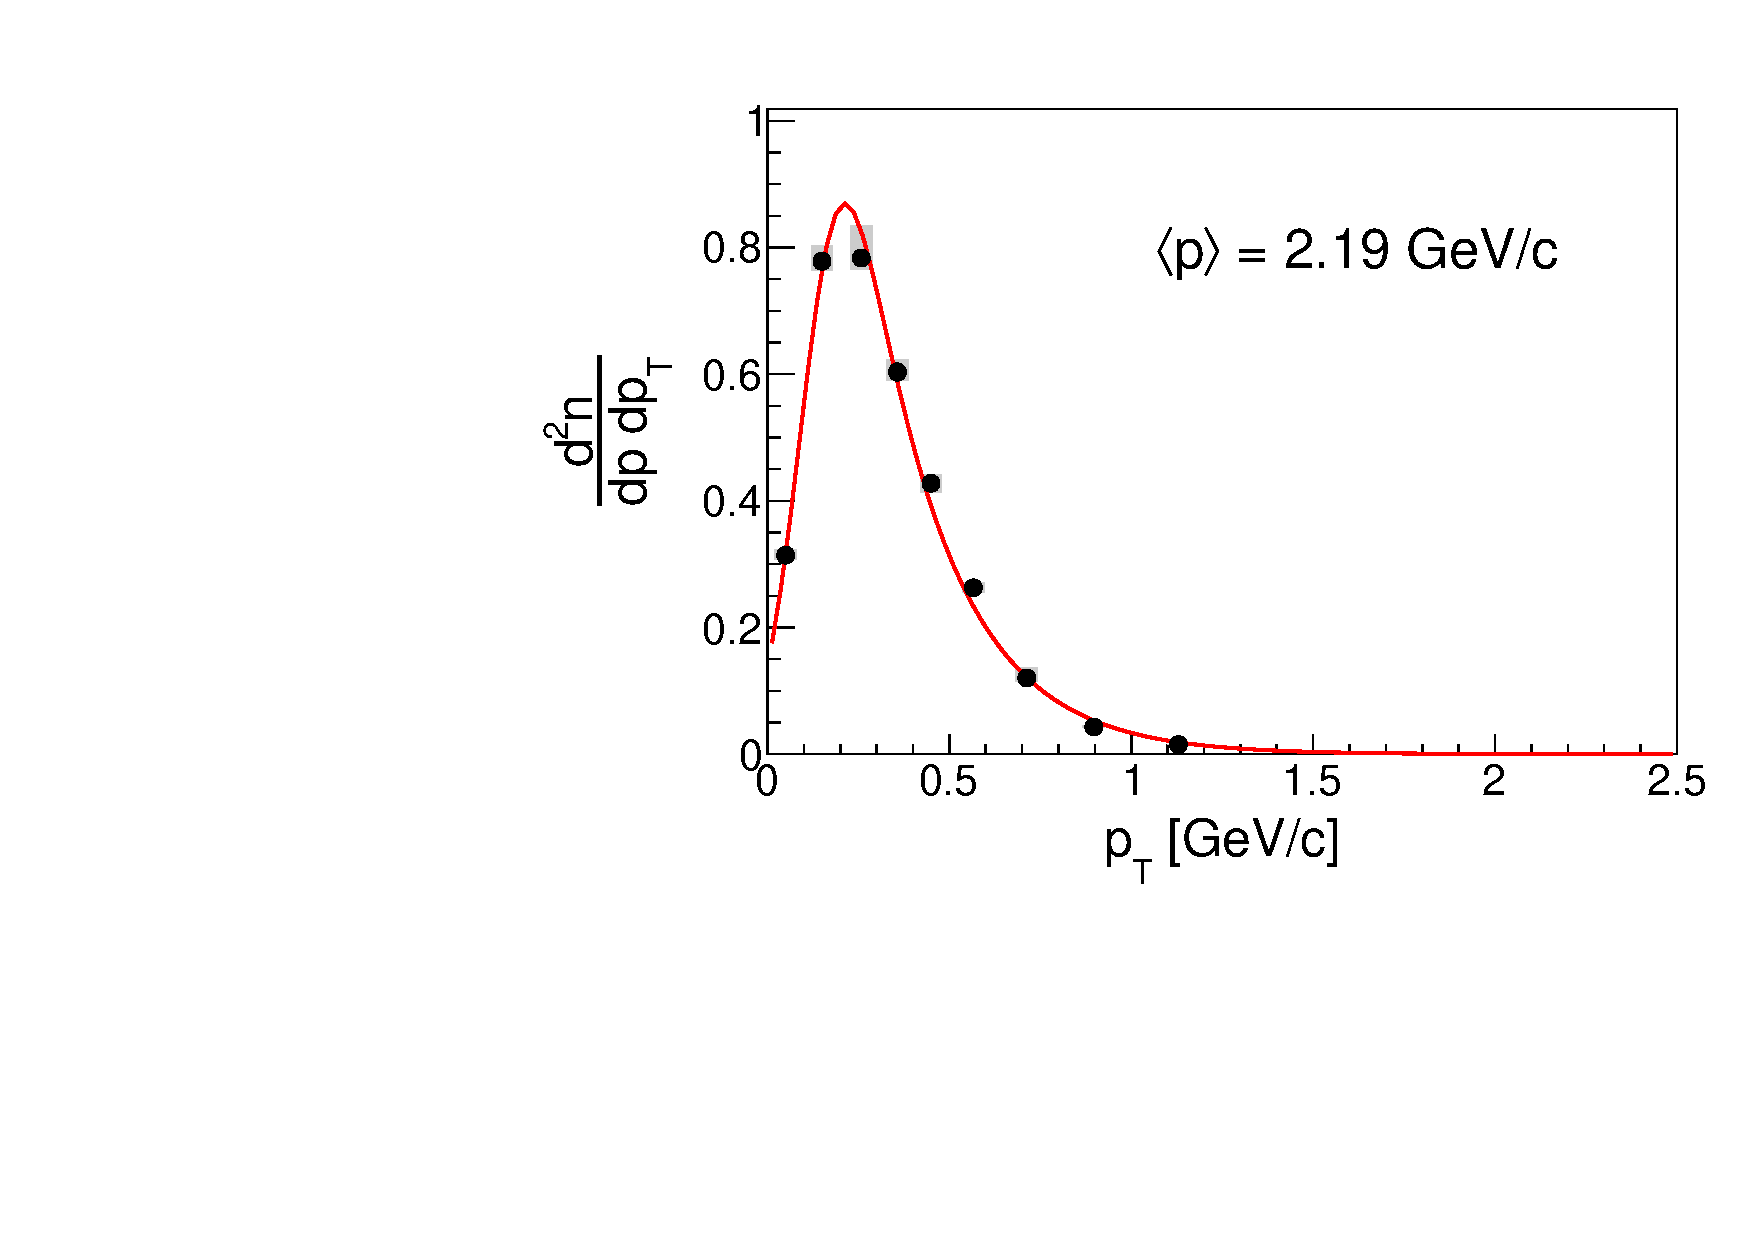
\includegraphics[clip, rviewport=0 0 1 1,width=0.24\textwidth]{spec/spec_pt_158_c0_p1_x13}
  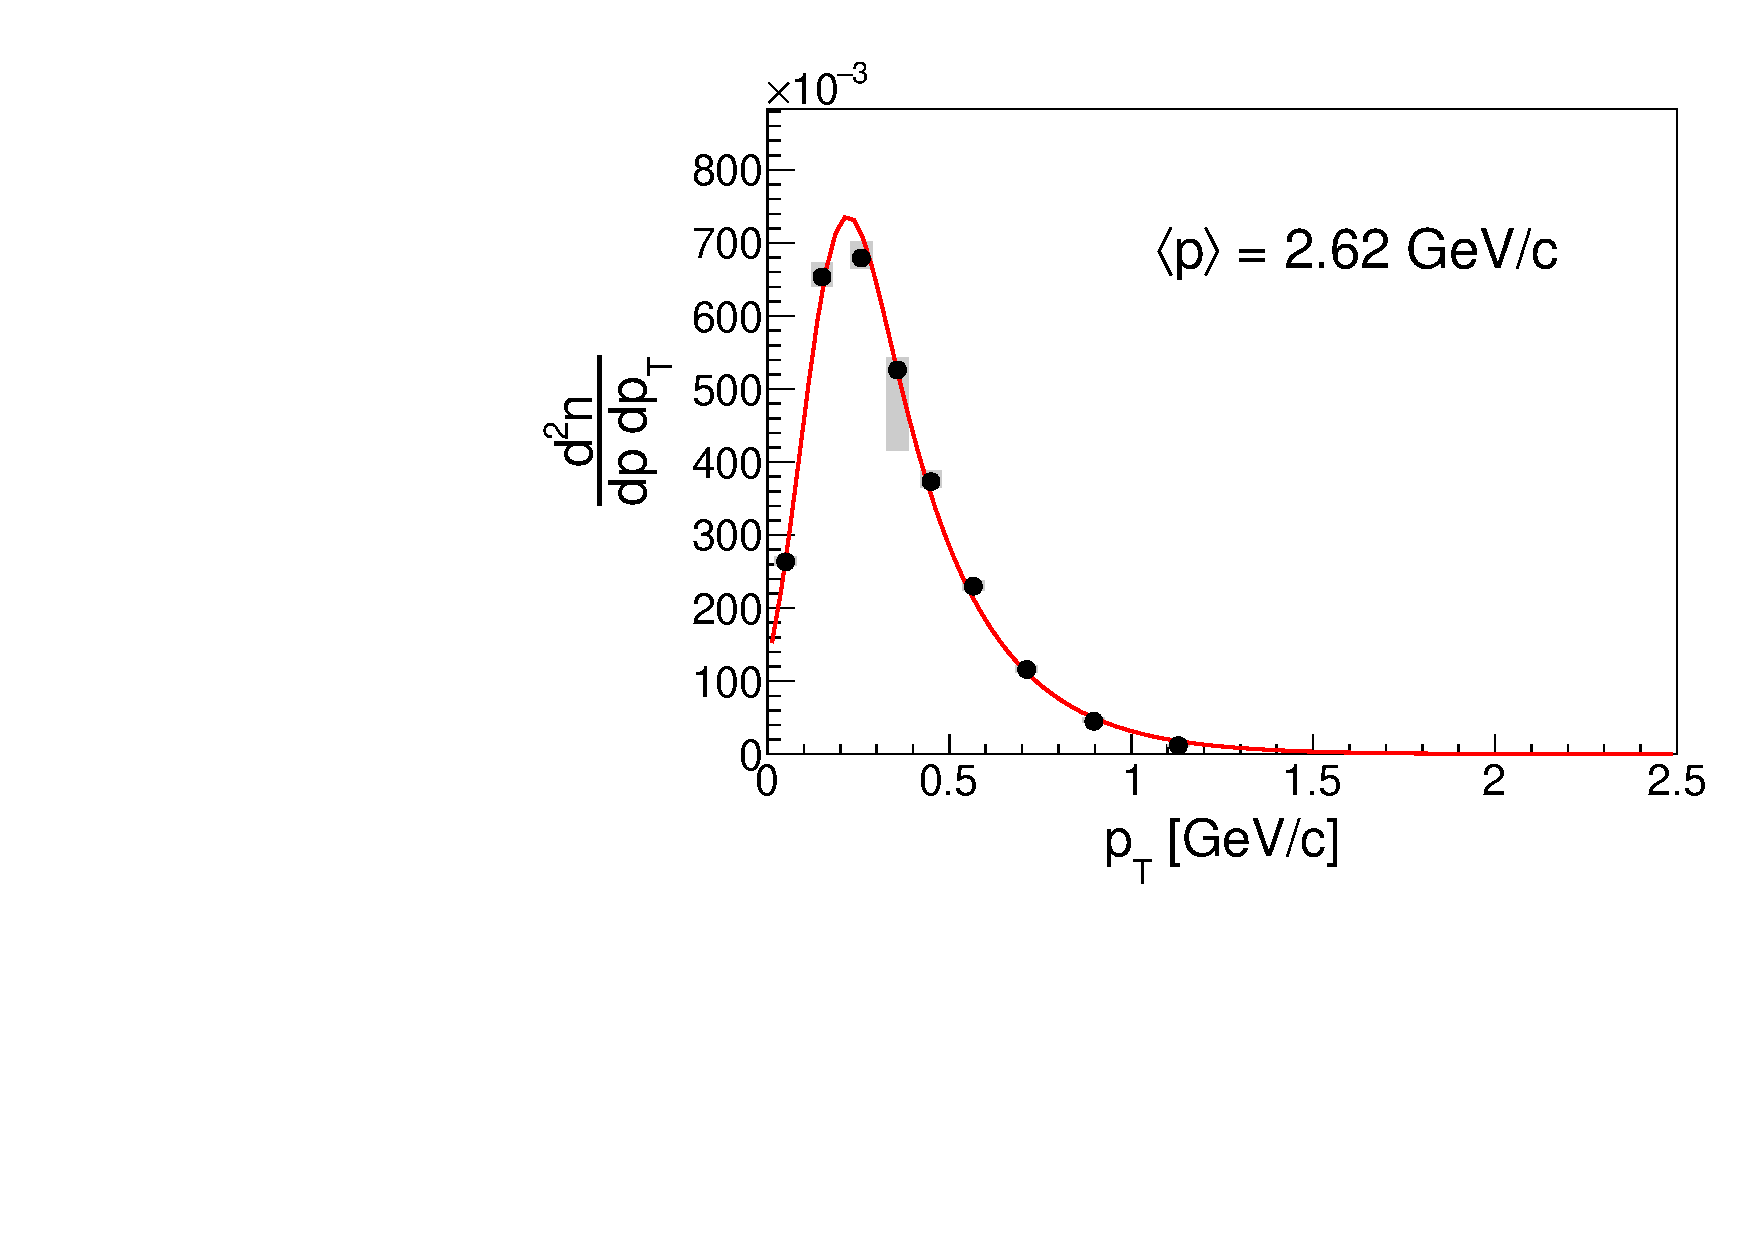
\includegraphics[clip, rviewport=0 0 1 1,width=0.24\textwidth]{spec/spec_pt_158_c0_p1_x14}
  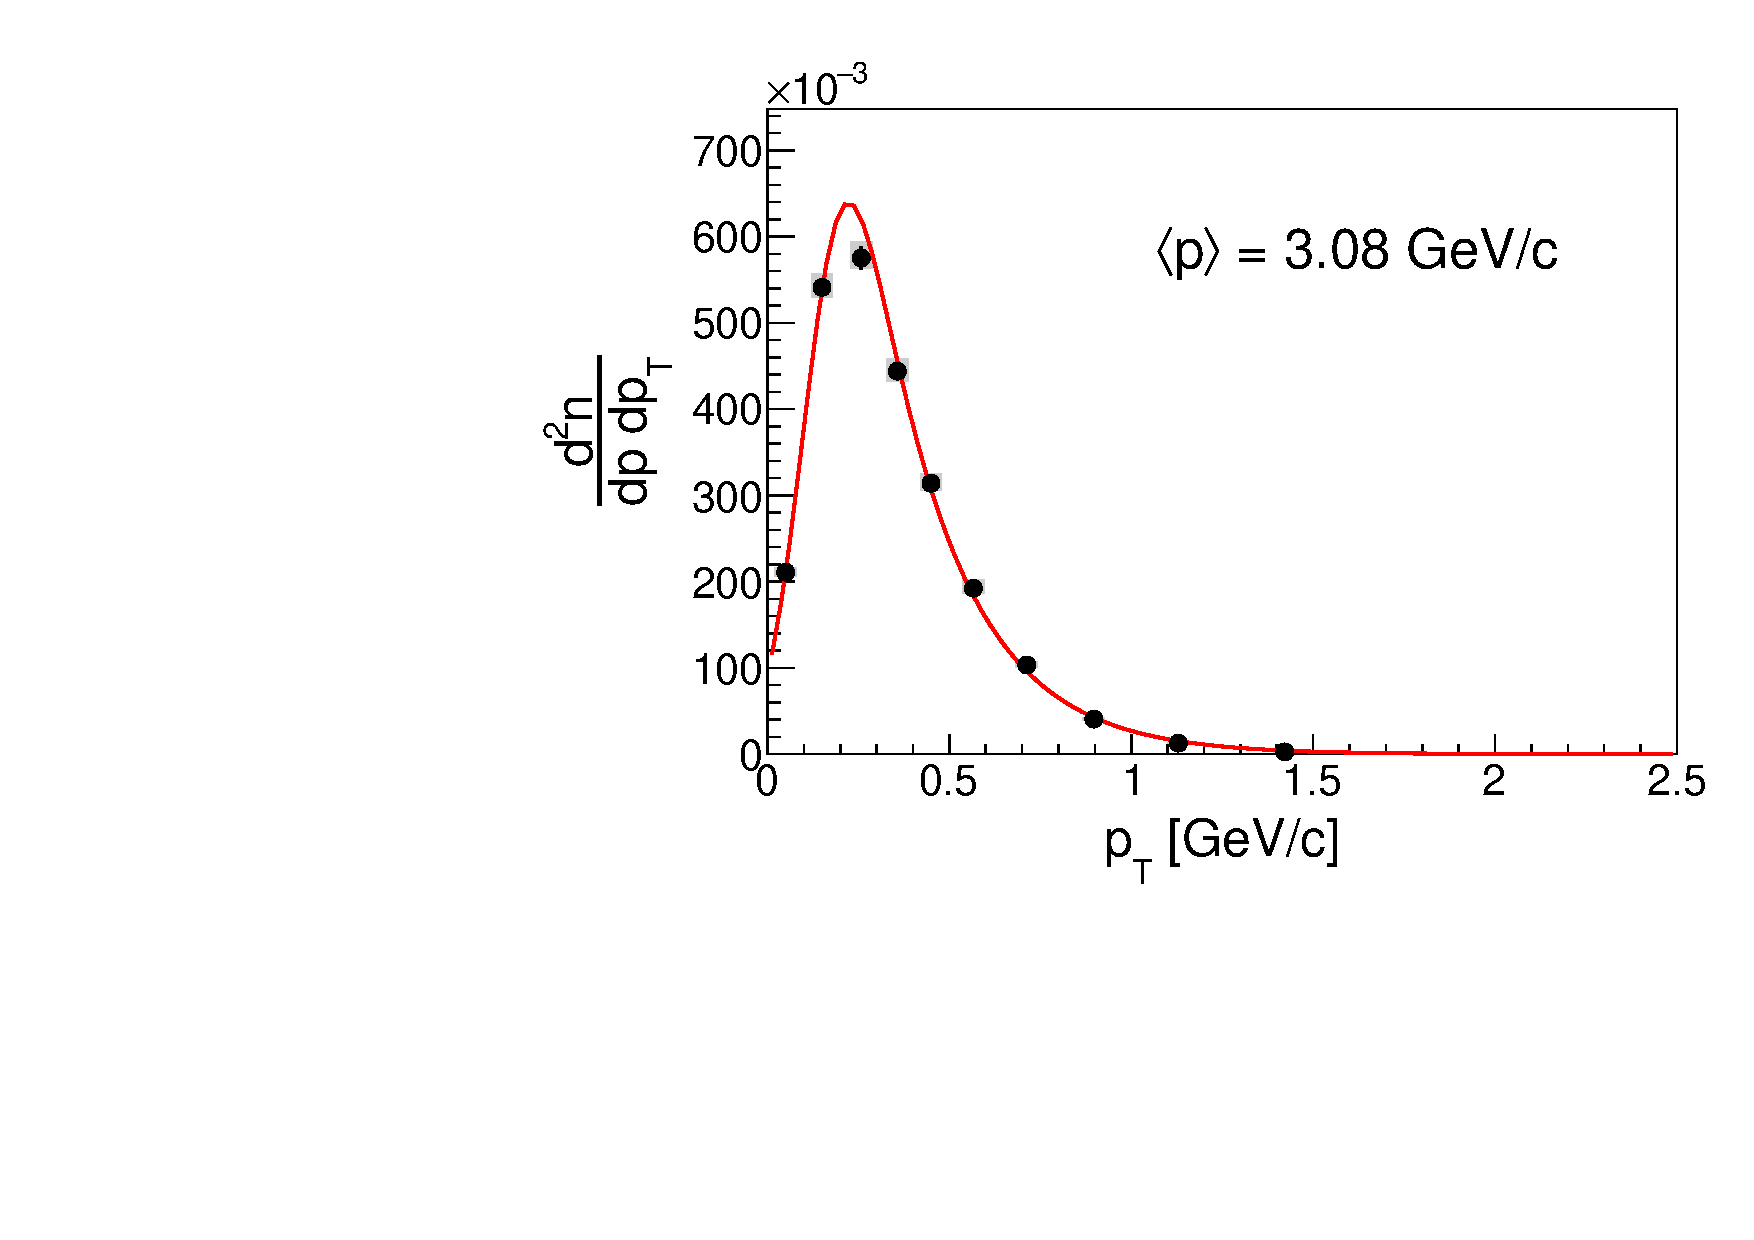
\includegraphics[clip, rviewport=0 0 1 1,width=0.24\textwidth]{spec/spec_pt_158_c0_p1_x15}
  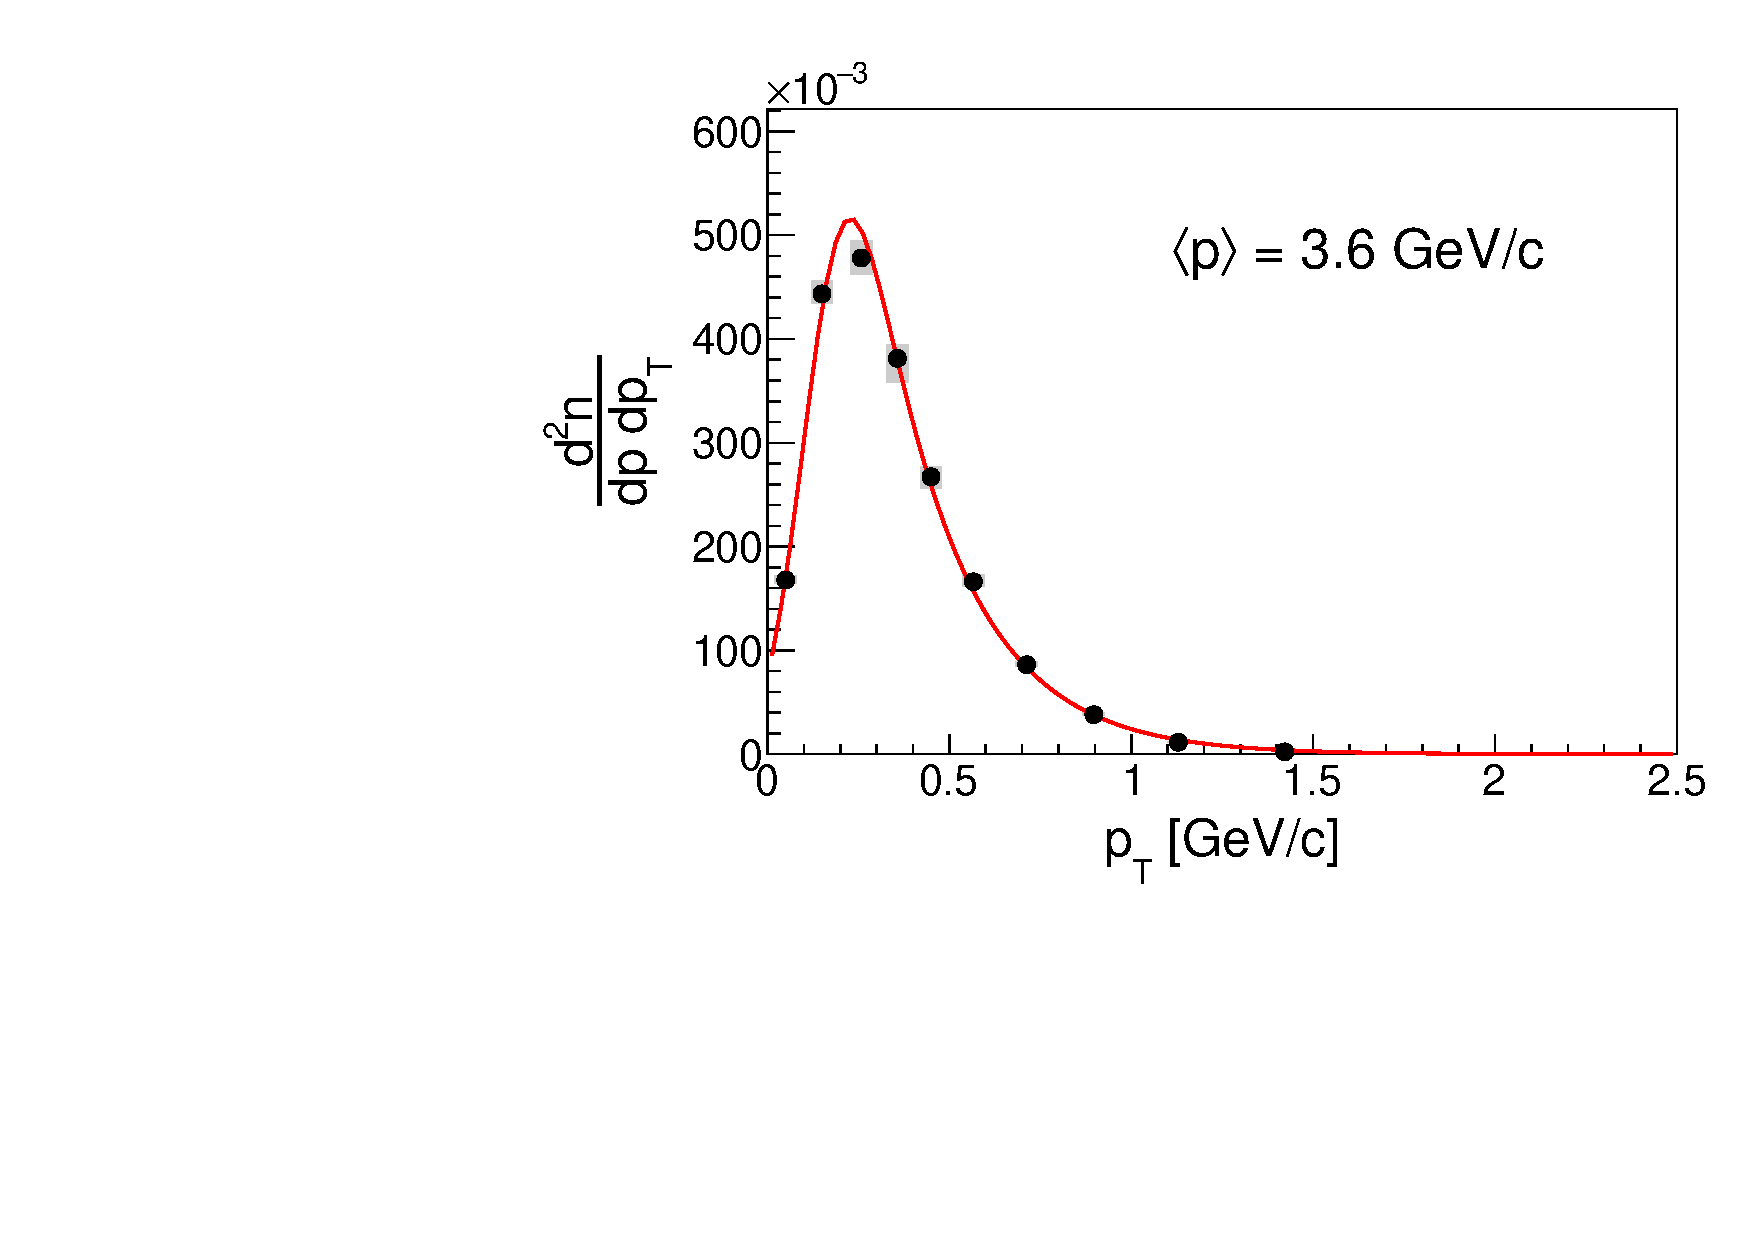
\includegraphics[clip, rviewport=0 0 1 1,width=0.24\textwidth]{spec/spec_pt_158_c0_p1_x16}

  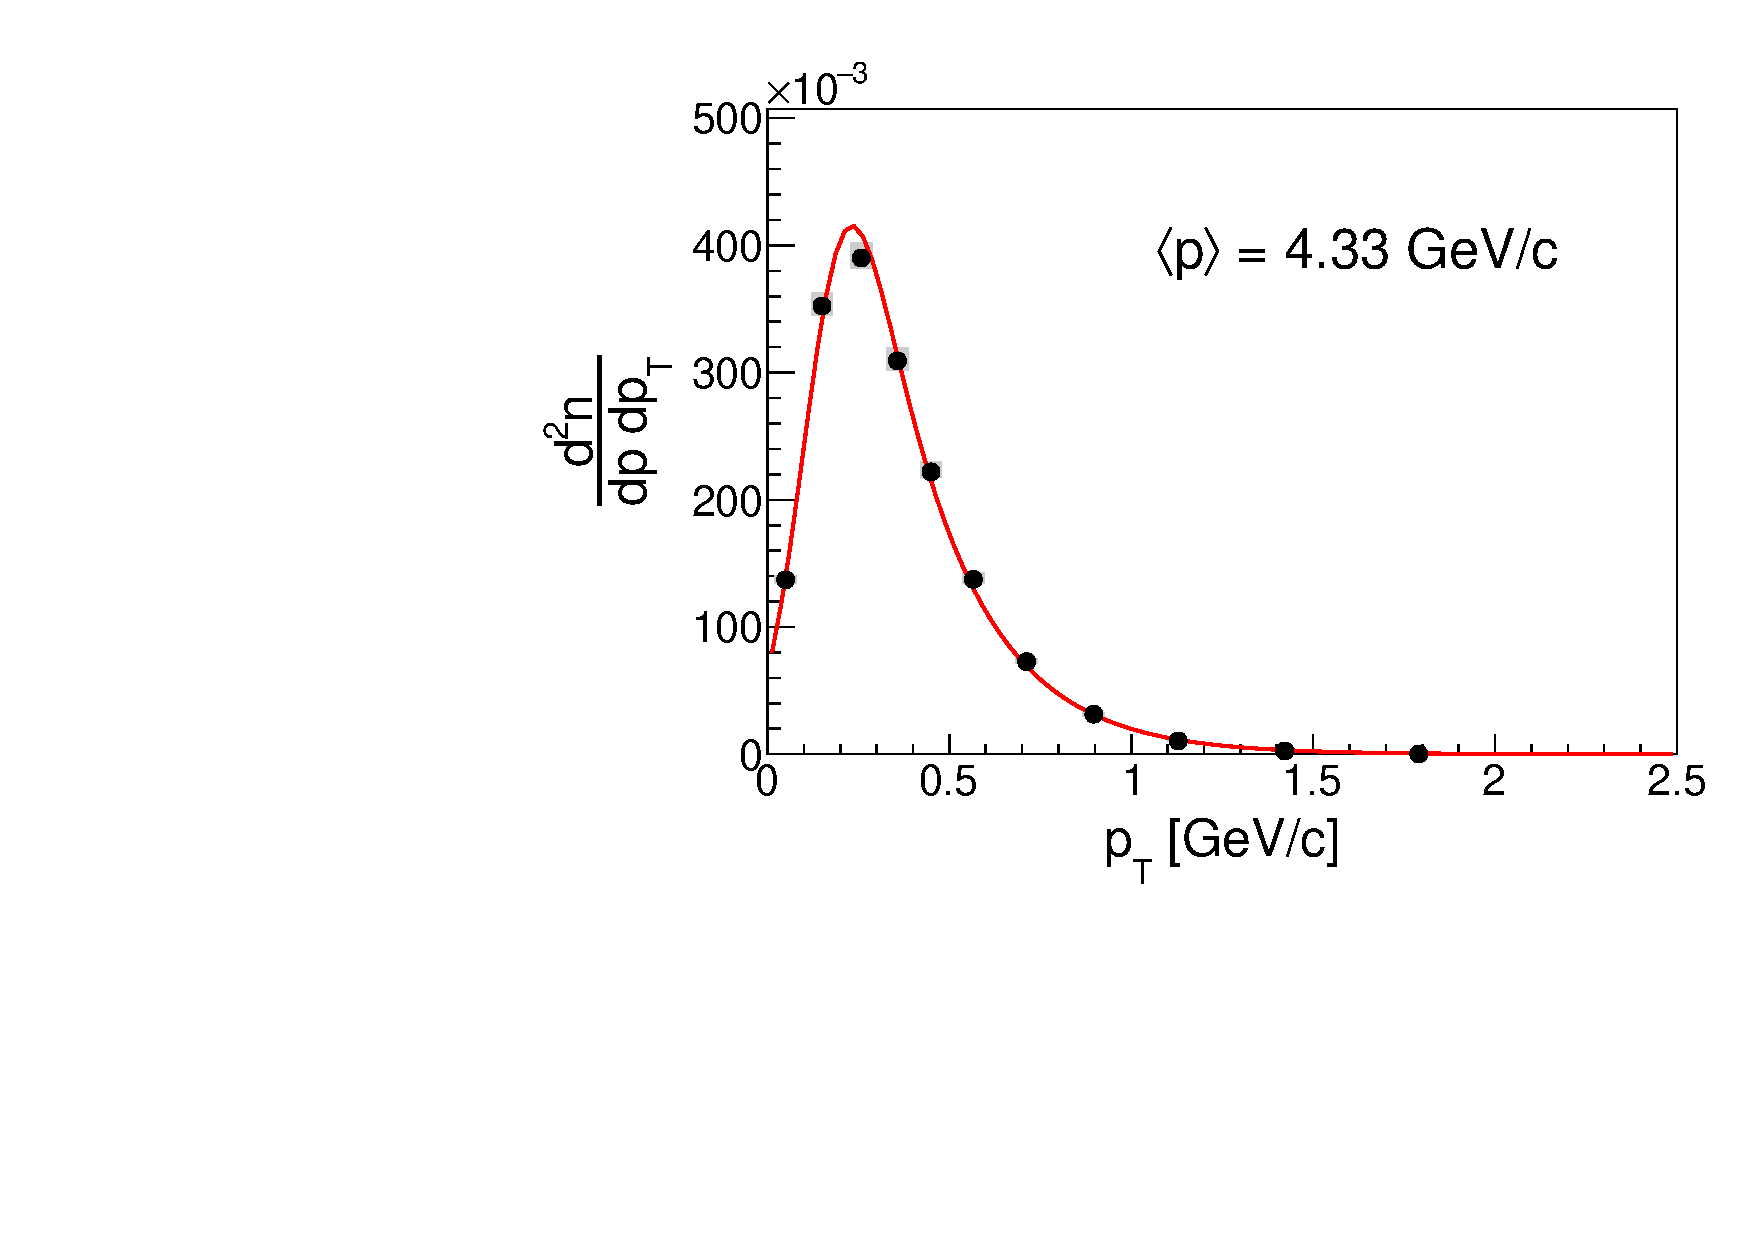
\includegraphics[clip, rviewport=0 0 1 1,width=0.24\textwidth]{spec/spec_pt_158_c0_p1_x17}
  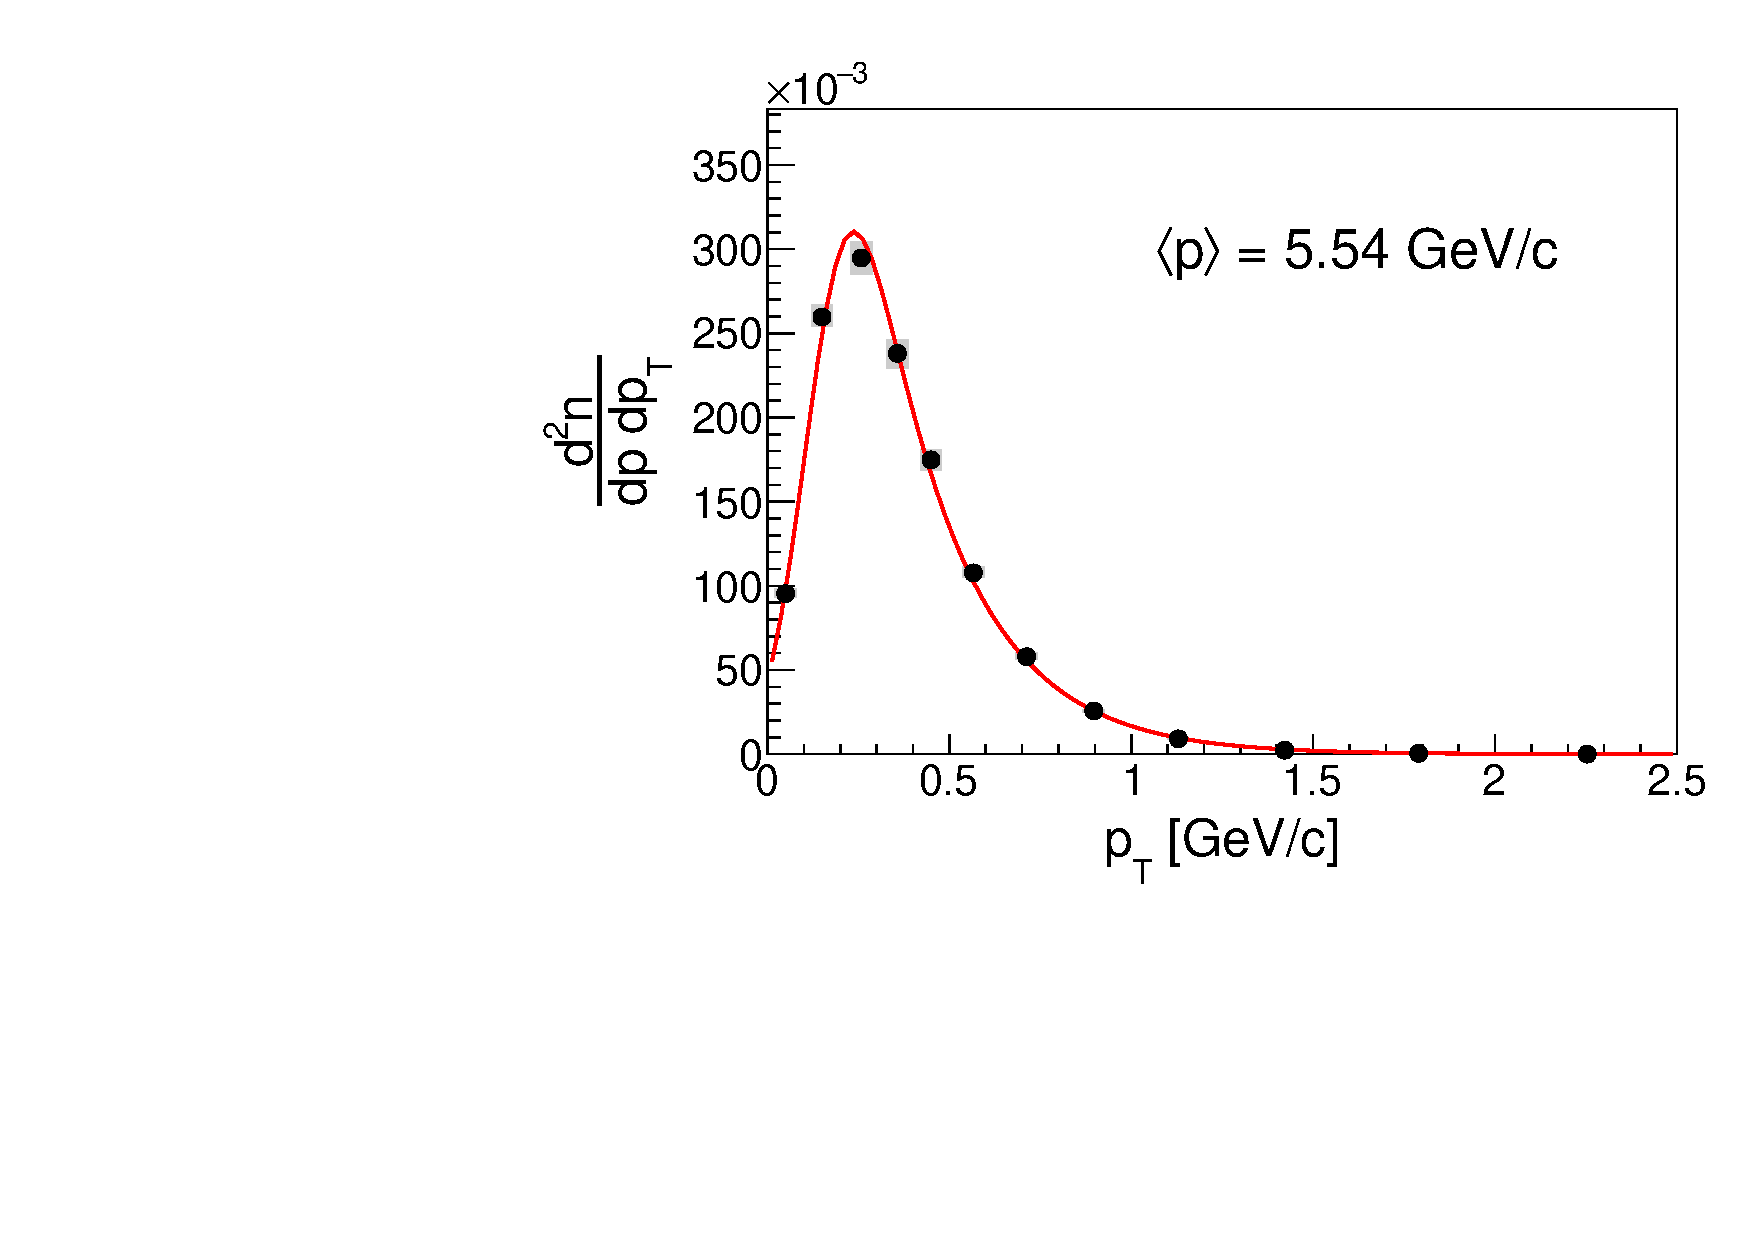
\includegraphics[clip, rviewport=0 0 1 1,width=0.24\textwidth]{spec/spec_pt_158_c0_p1_x18}
  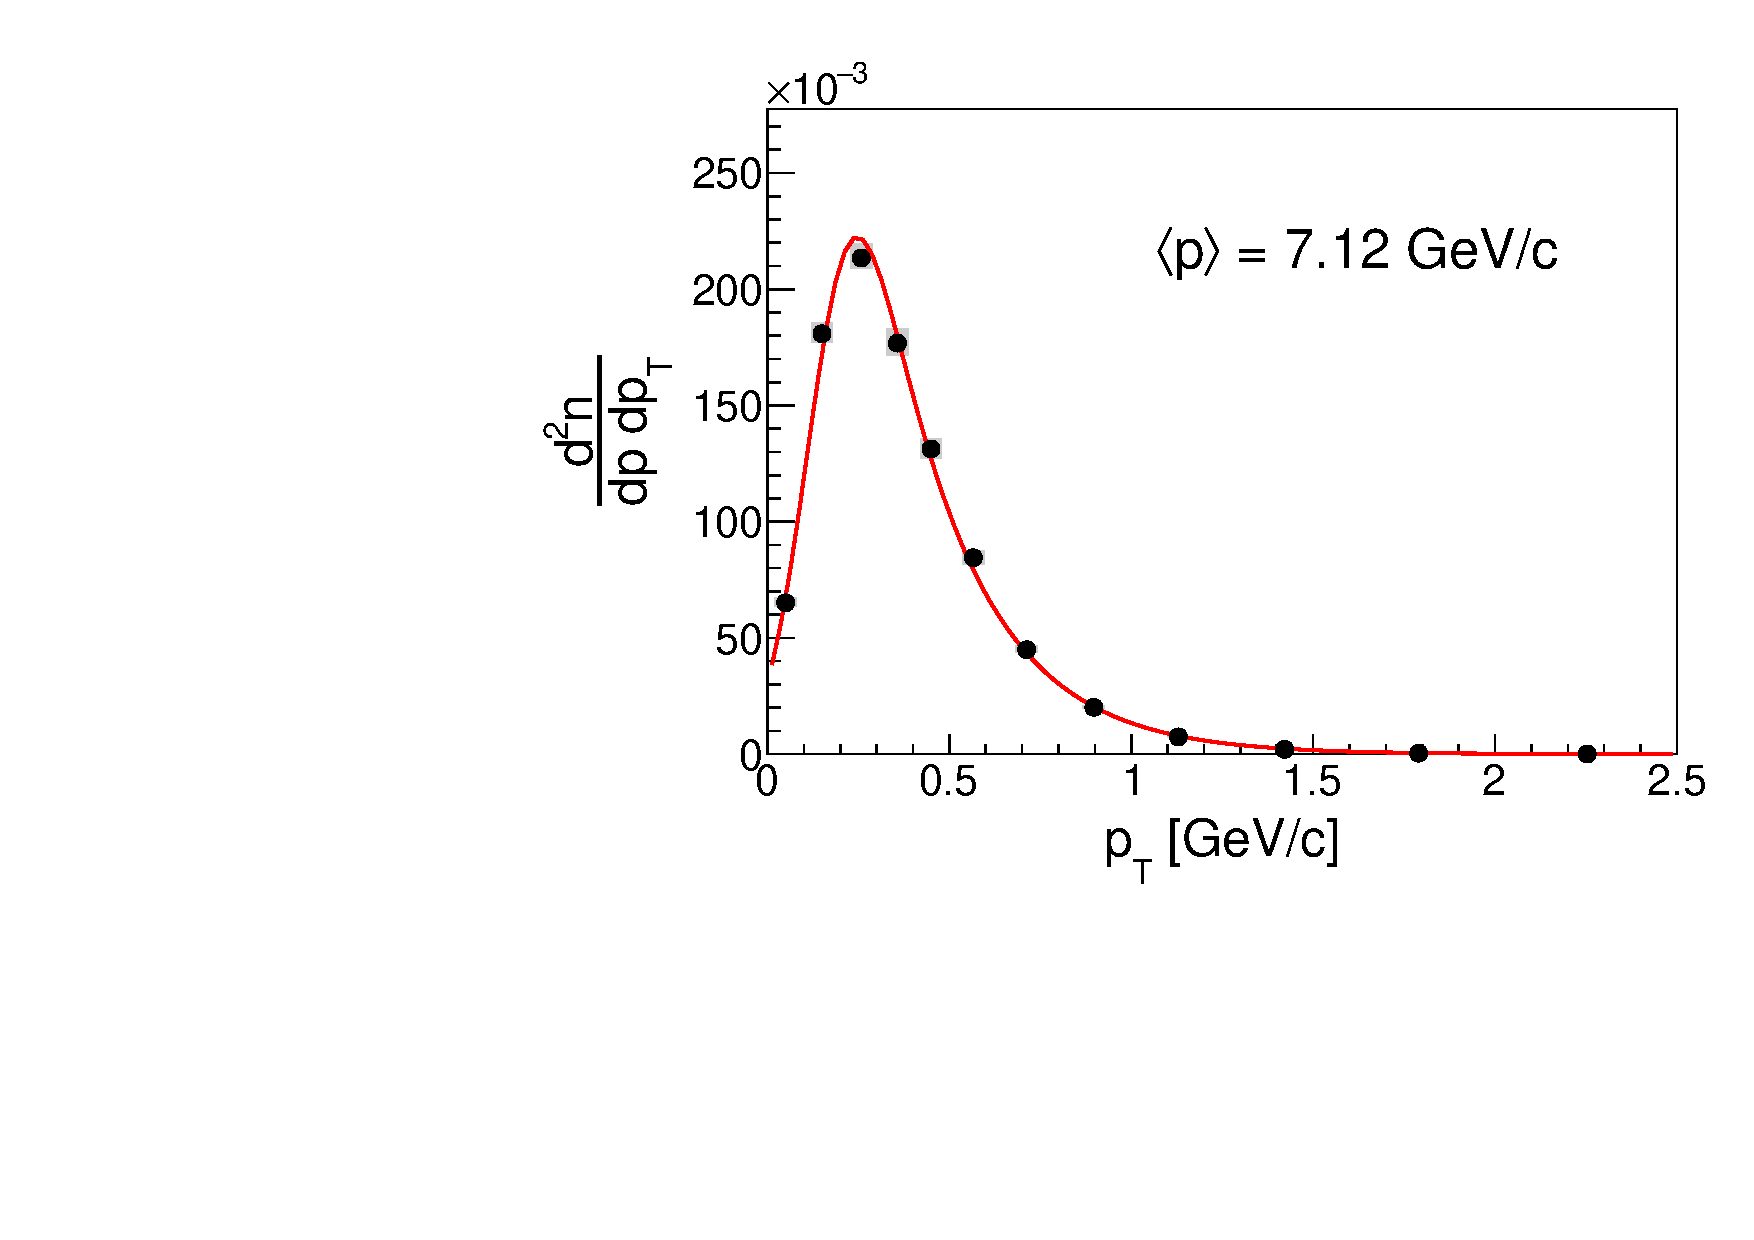
\includegraphics[clip, rviewport=0 0 1 1,width=0.24\textwidth]{spec/spec_pt_158_c0_p1_x19}
  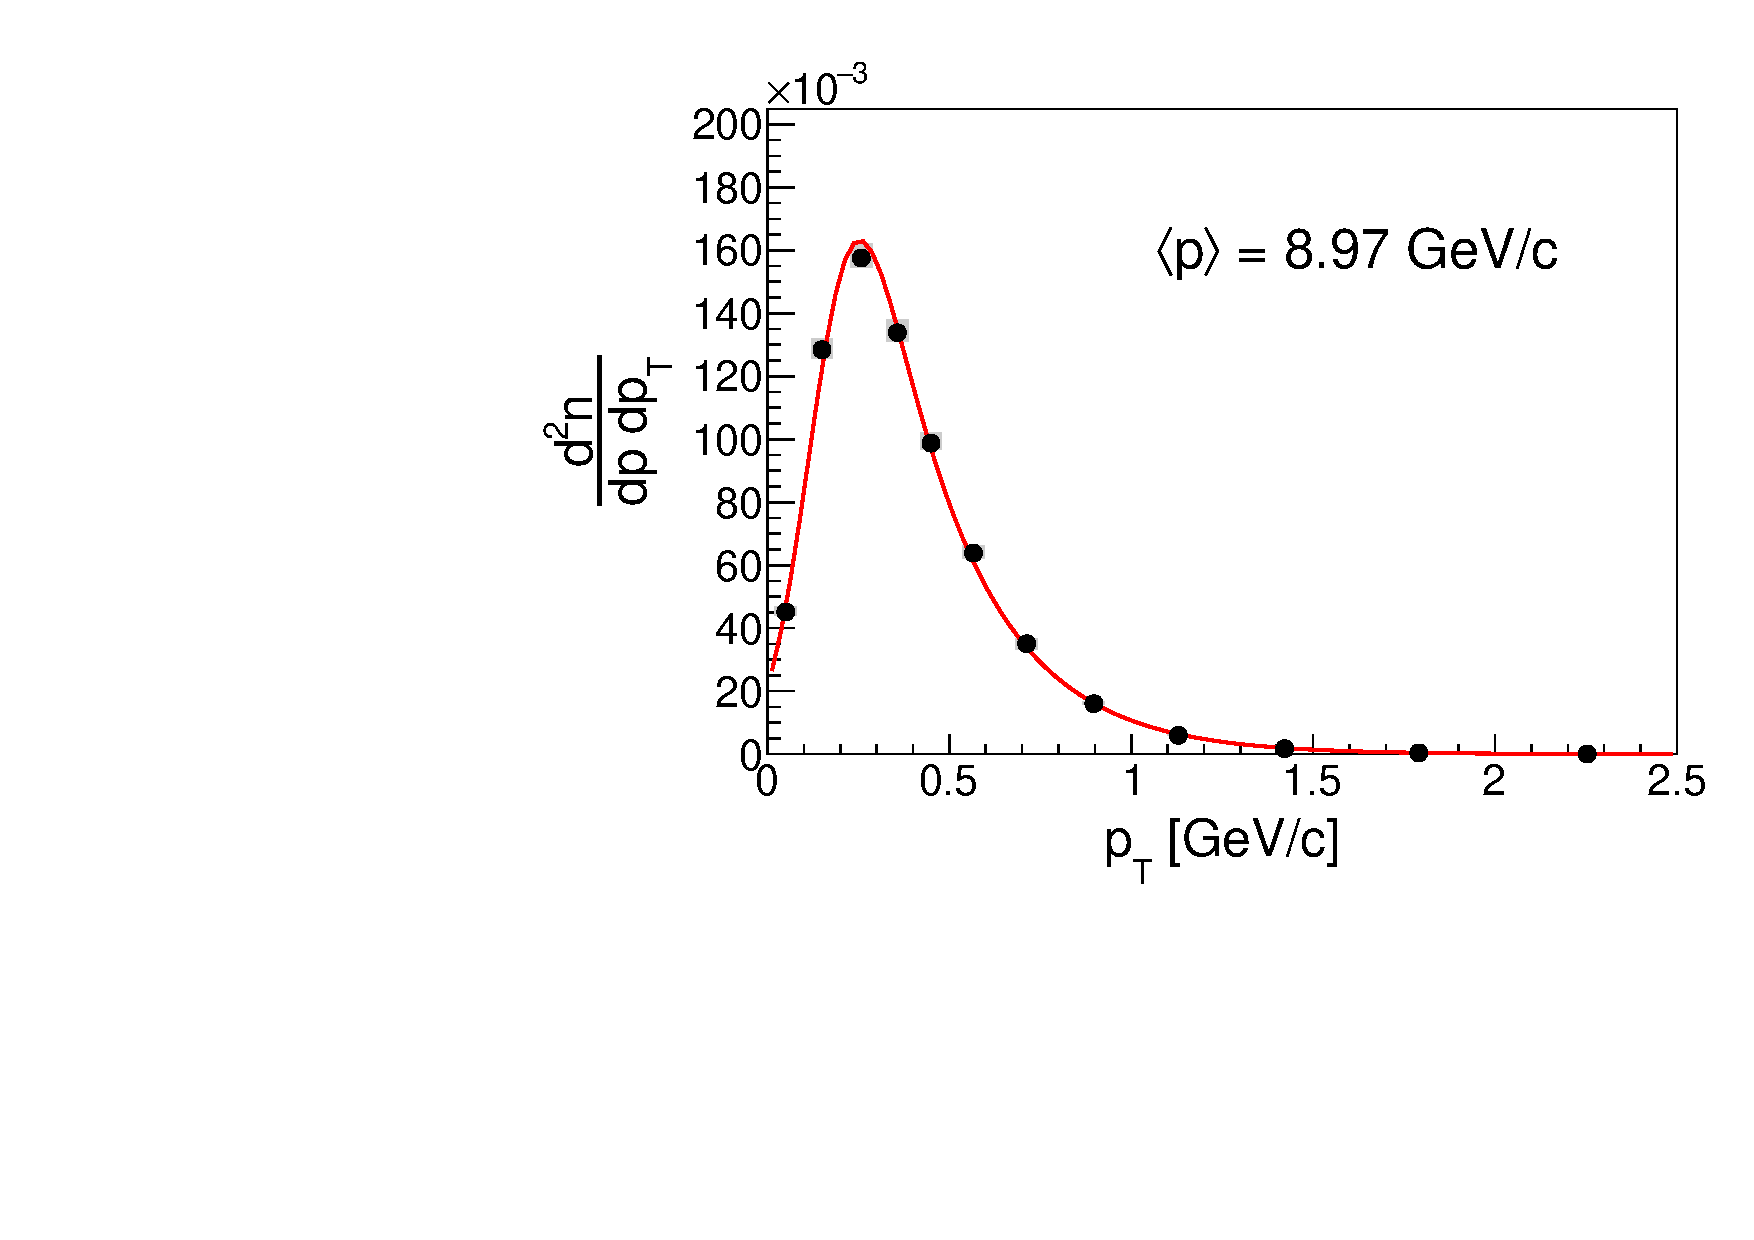
\includegraphics[clip, rviewport=0 0 1 1,width=0.24\textwidth]{spec/spec_pt_158_c0_p1_x20}

  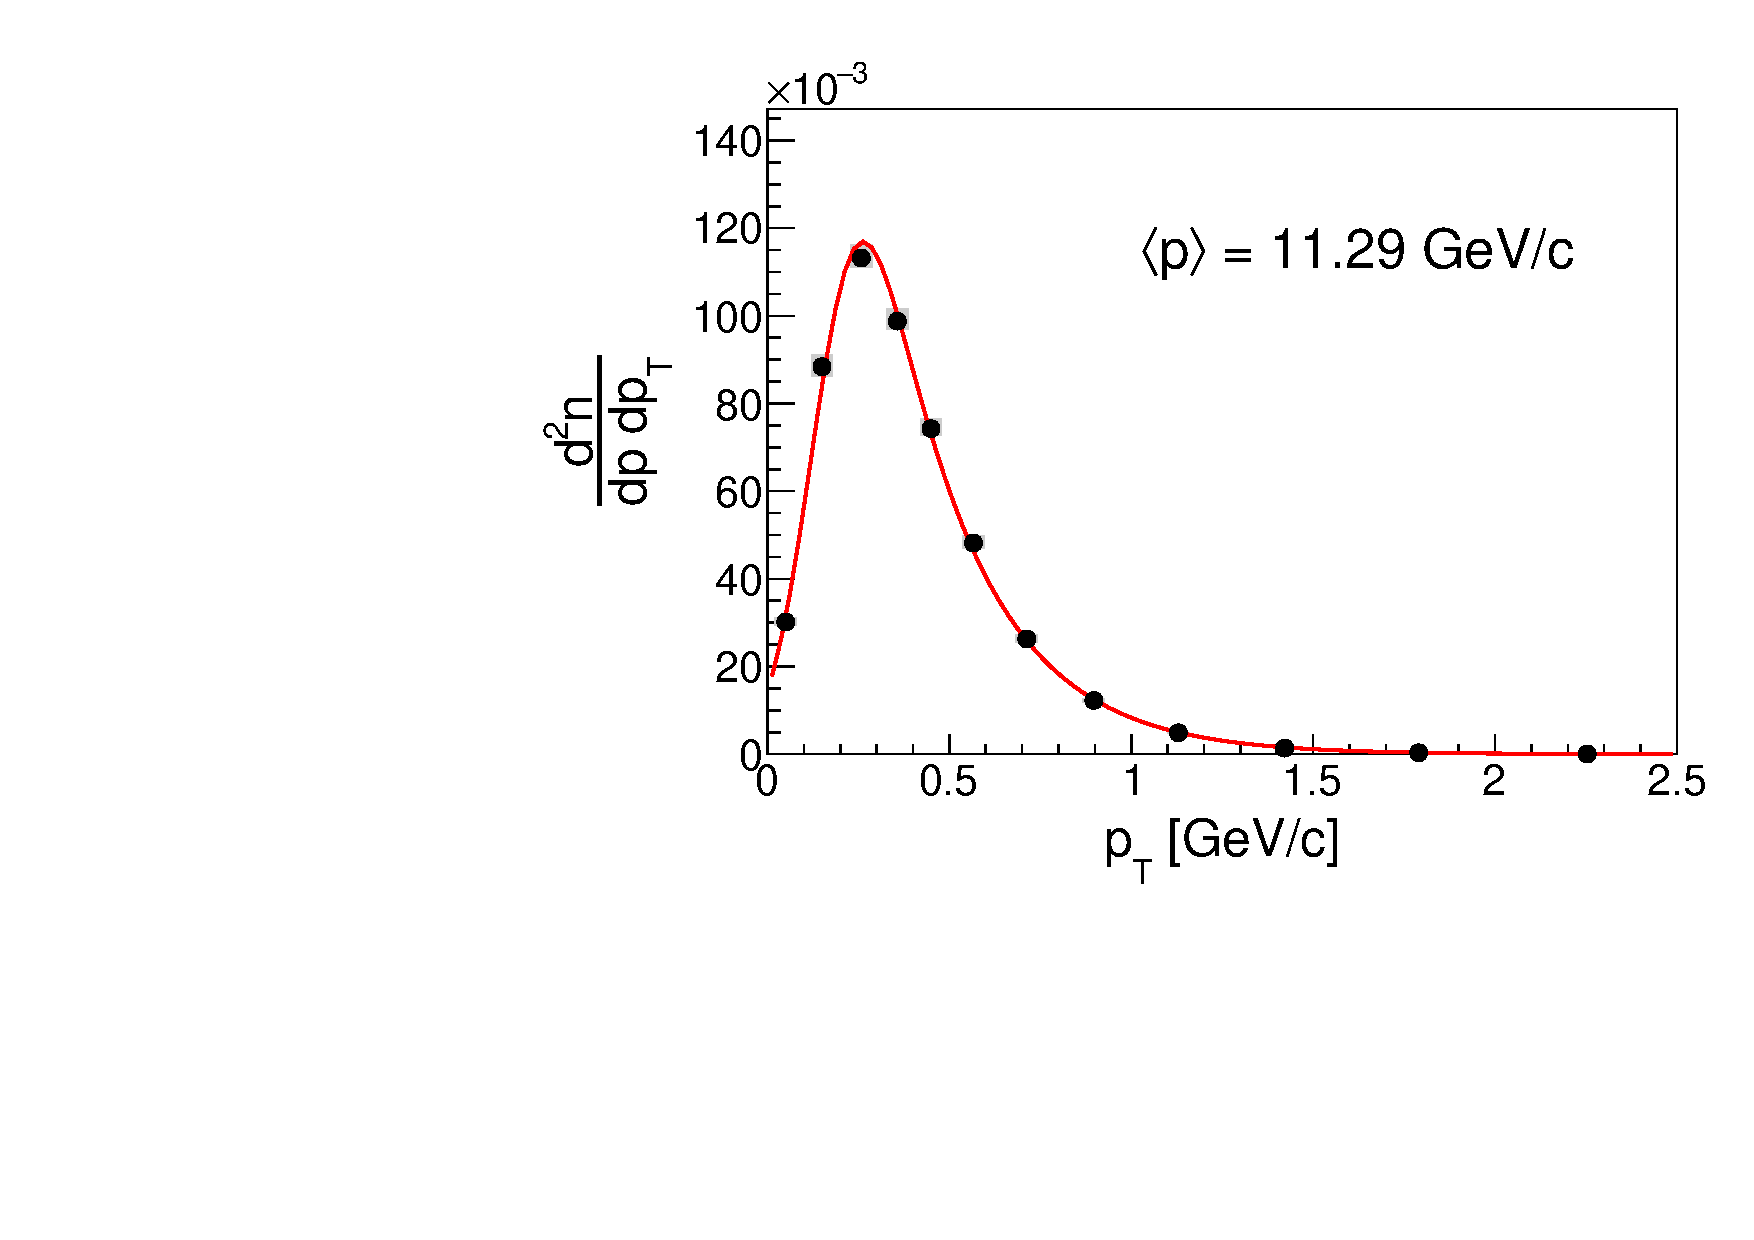
\includegraphics[clip, rviewport=0 0 1 1,width=0.24\textwidth]{spec/spec_pt_158_c0_p1_x21}
  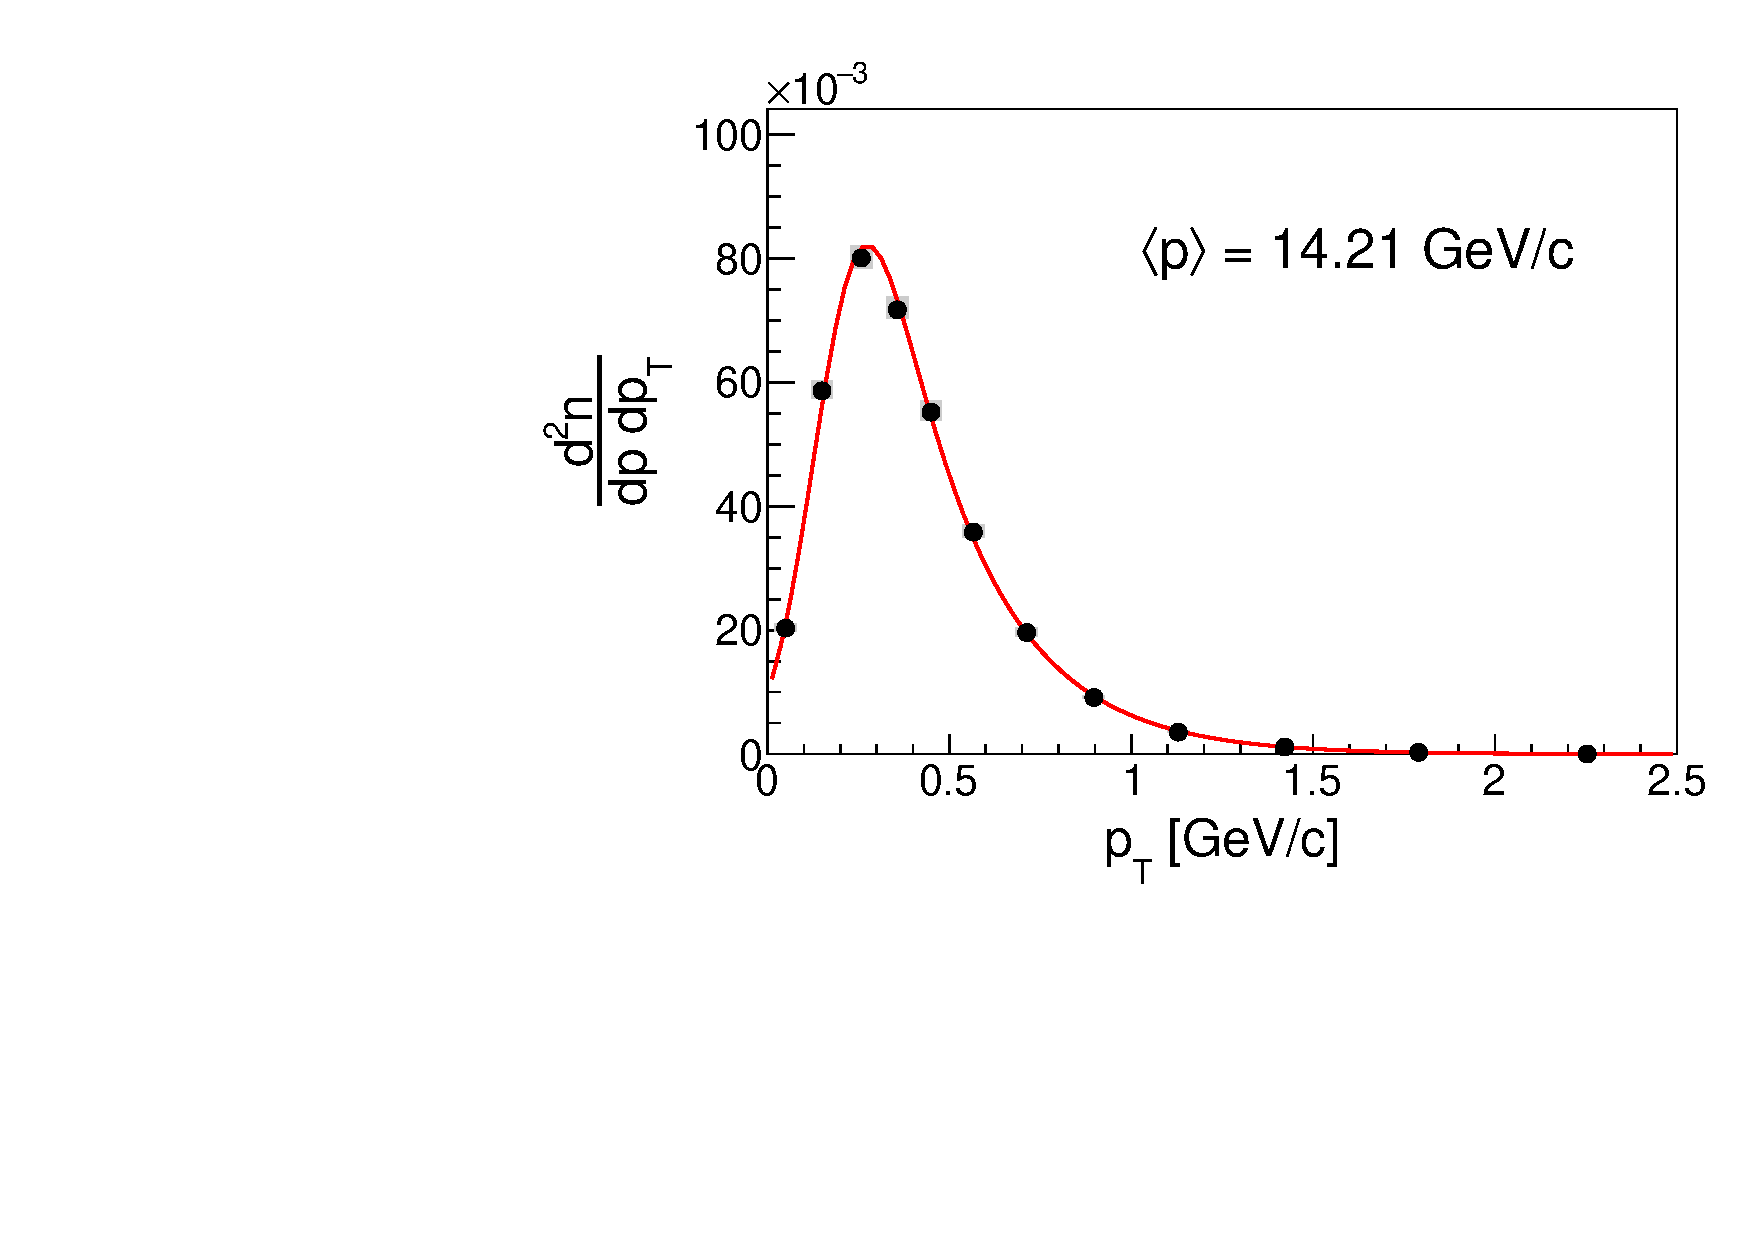
\includegraphics[clip, rviewport=0 0 1 1,width=0.24\textwidth]{spec/spec_pt_158_c0_p1_x22}
  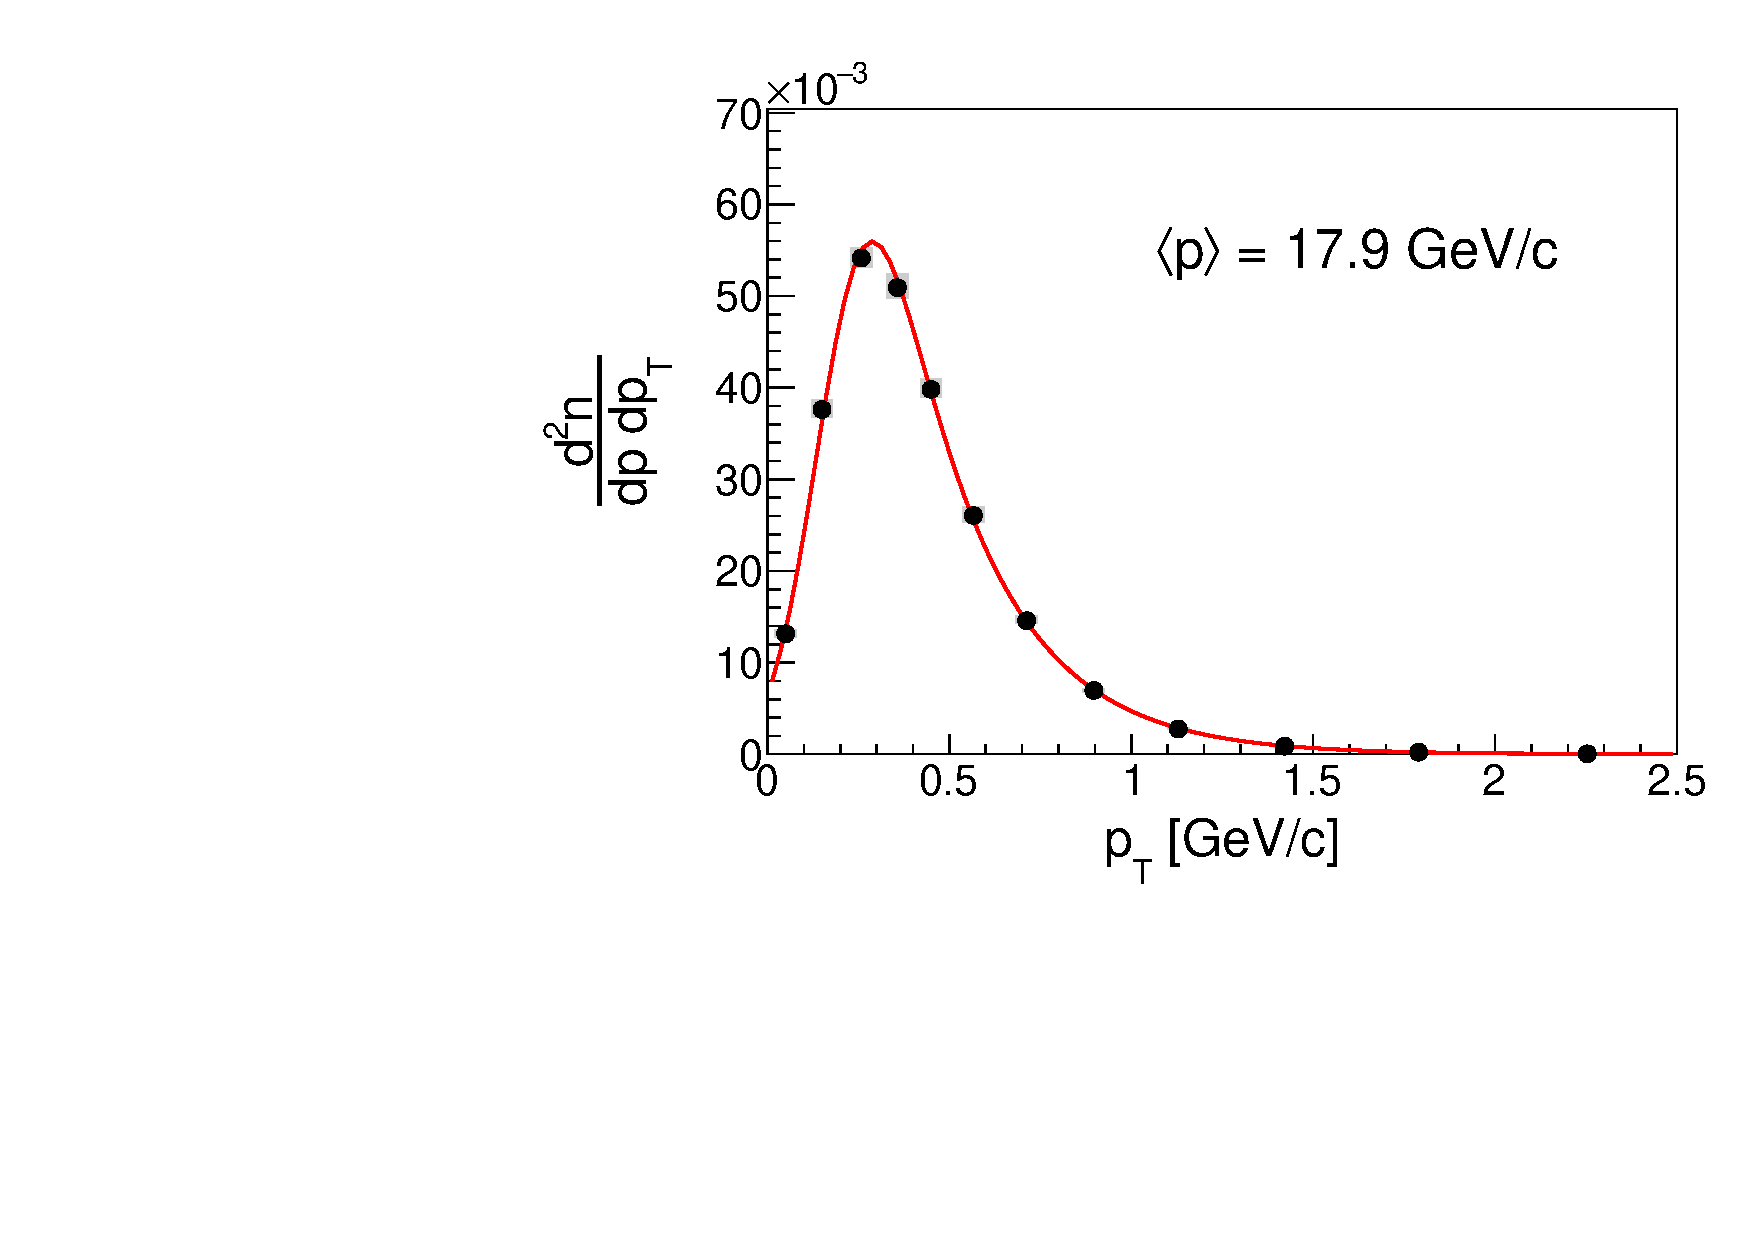
\includegraphics[clip, rviewport=0 0 1 1,width=0.24\textwidth]{spec/spec_pt_158_c0_p1_x23}
  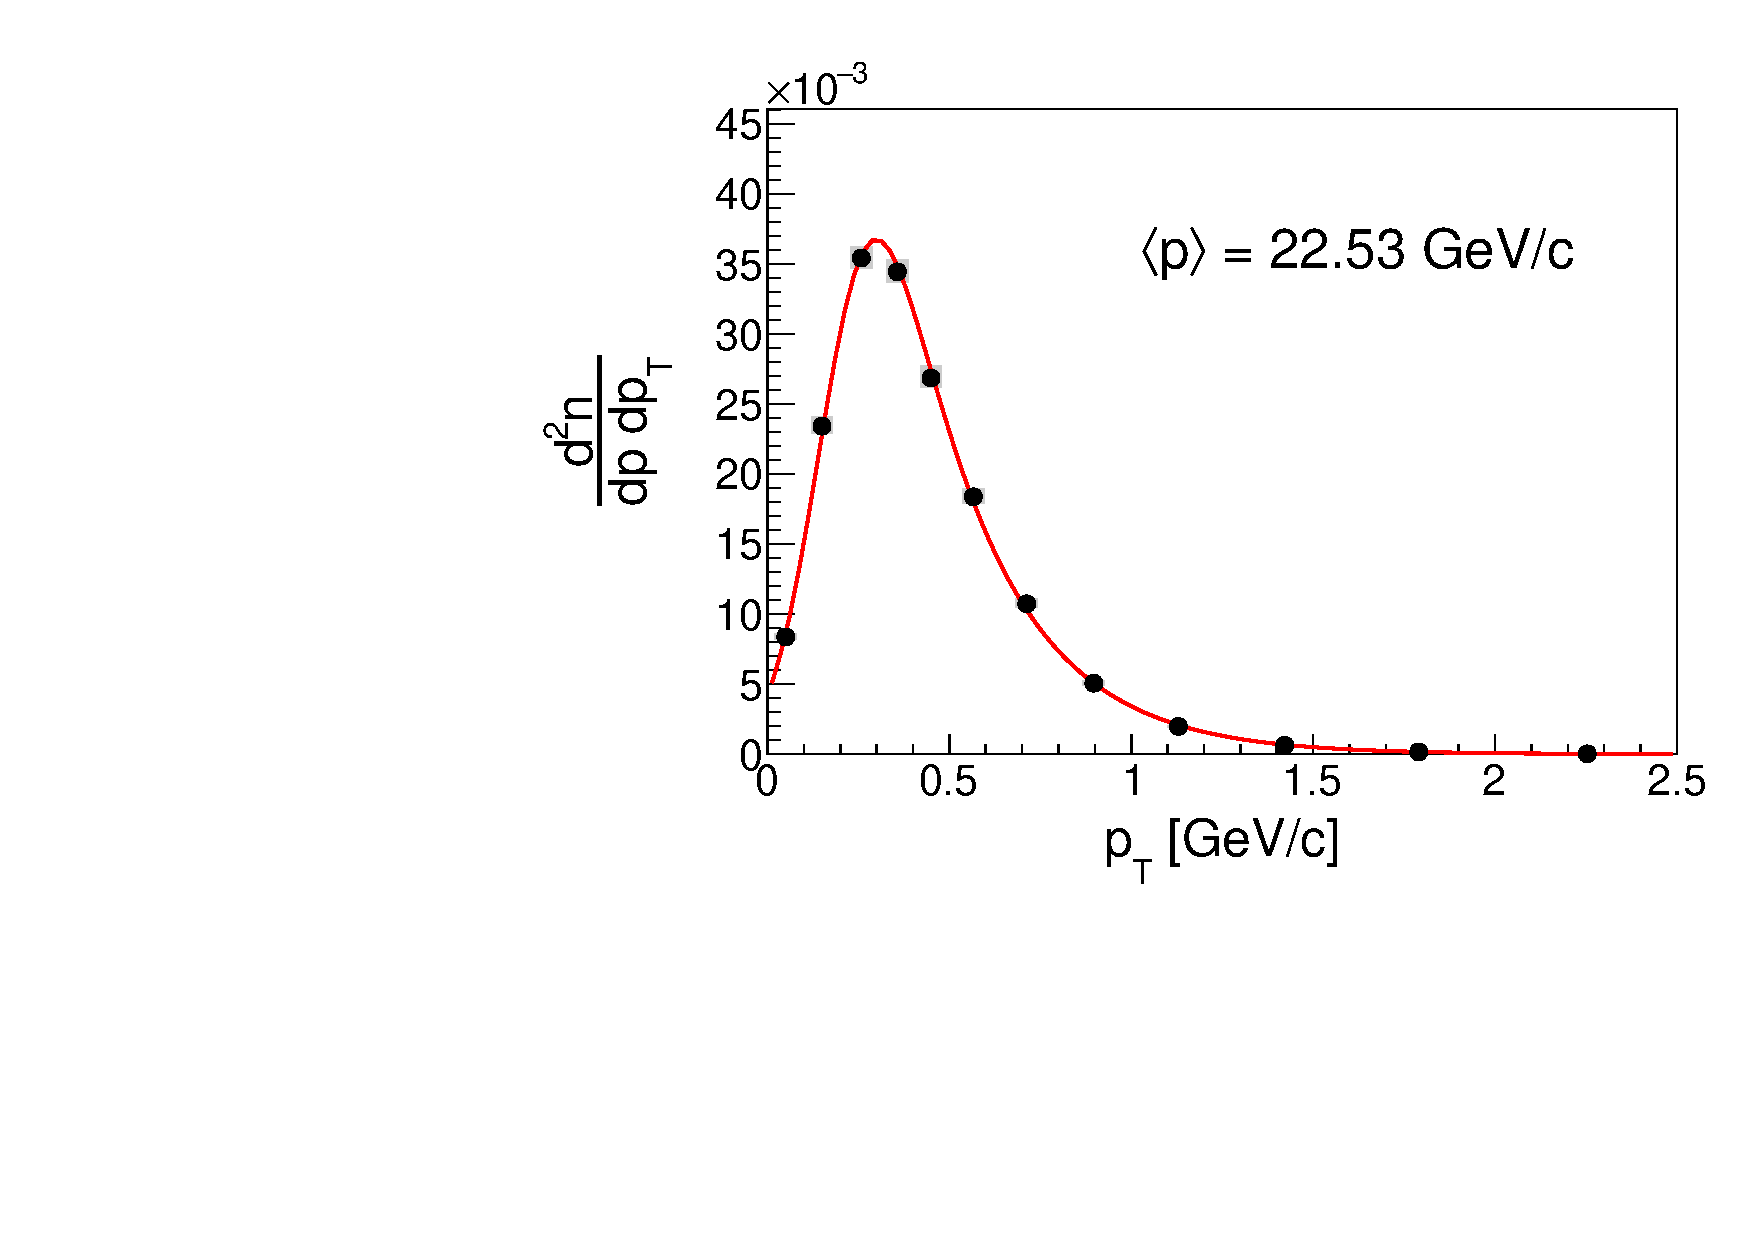
\includegraphics[clip, rviewport=0 0 1 1,width=0.24\textwidth]{spec/spec_pt_158_c0_p1_x24}

  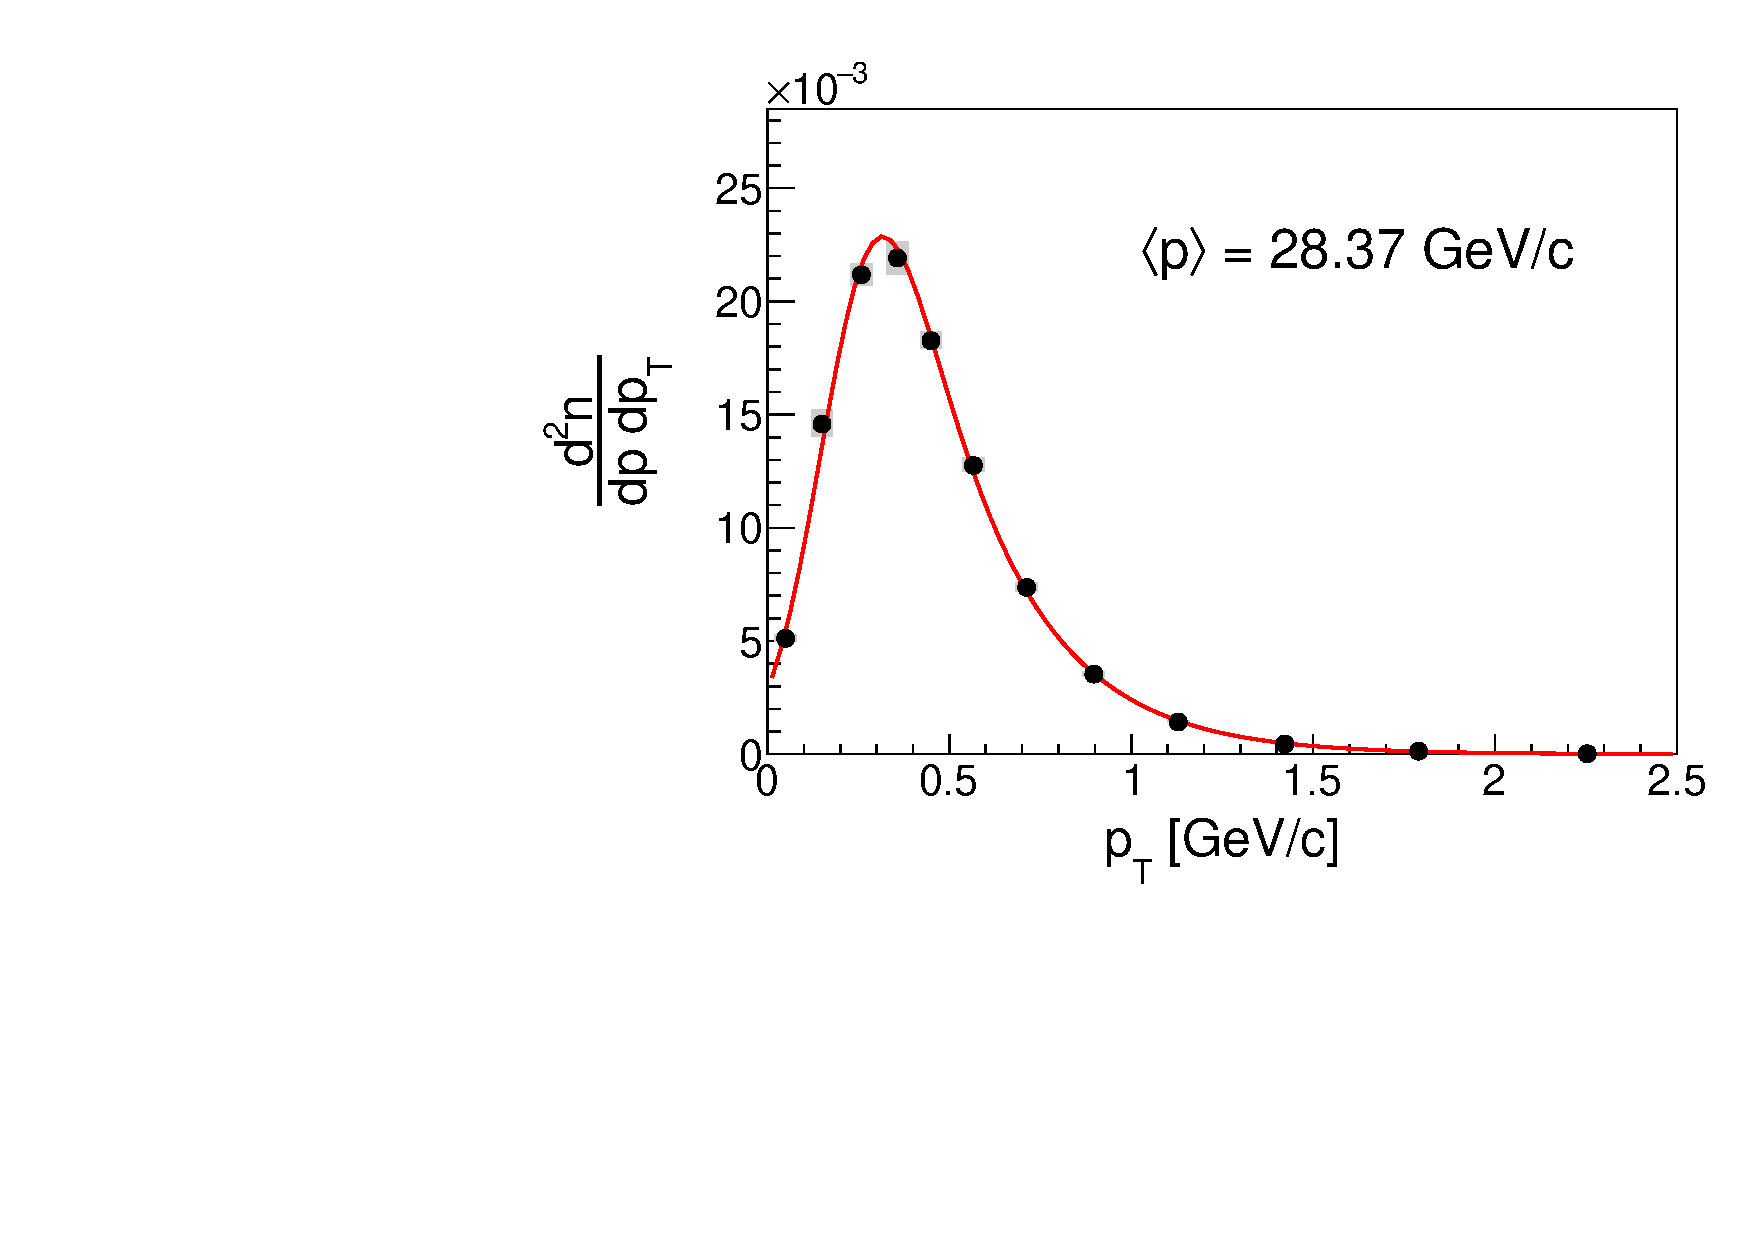
\includegraphics[clip, rviewport=0 0 1 1,width=0.24\textwidth]{spec/spec_pt_158_c0_p1_x25}
  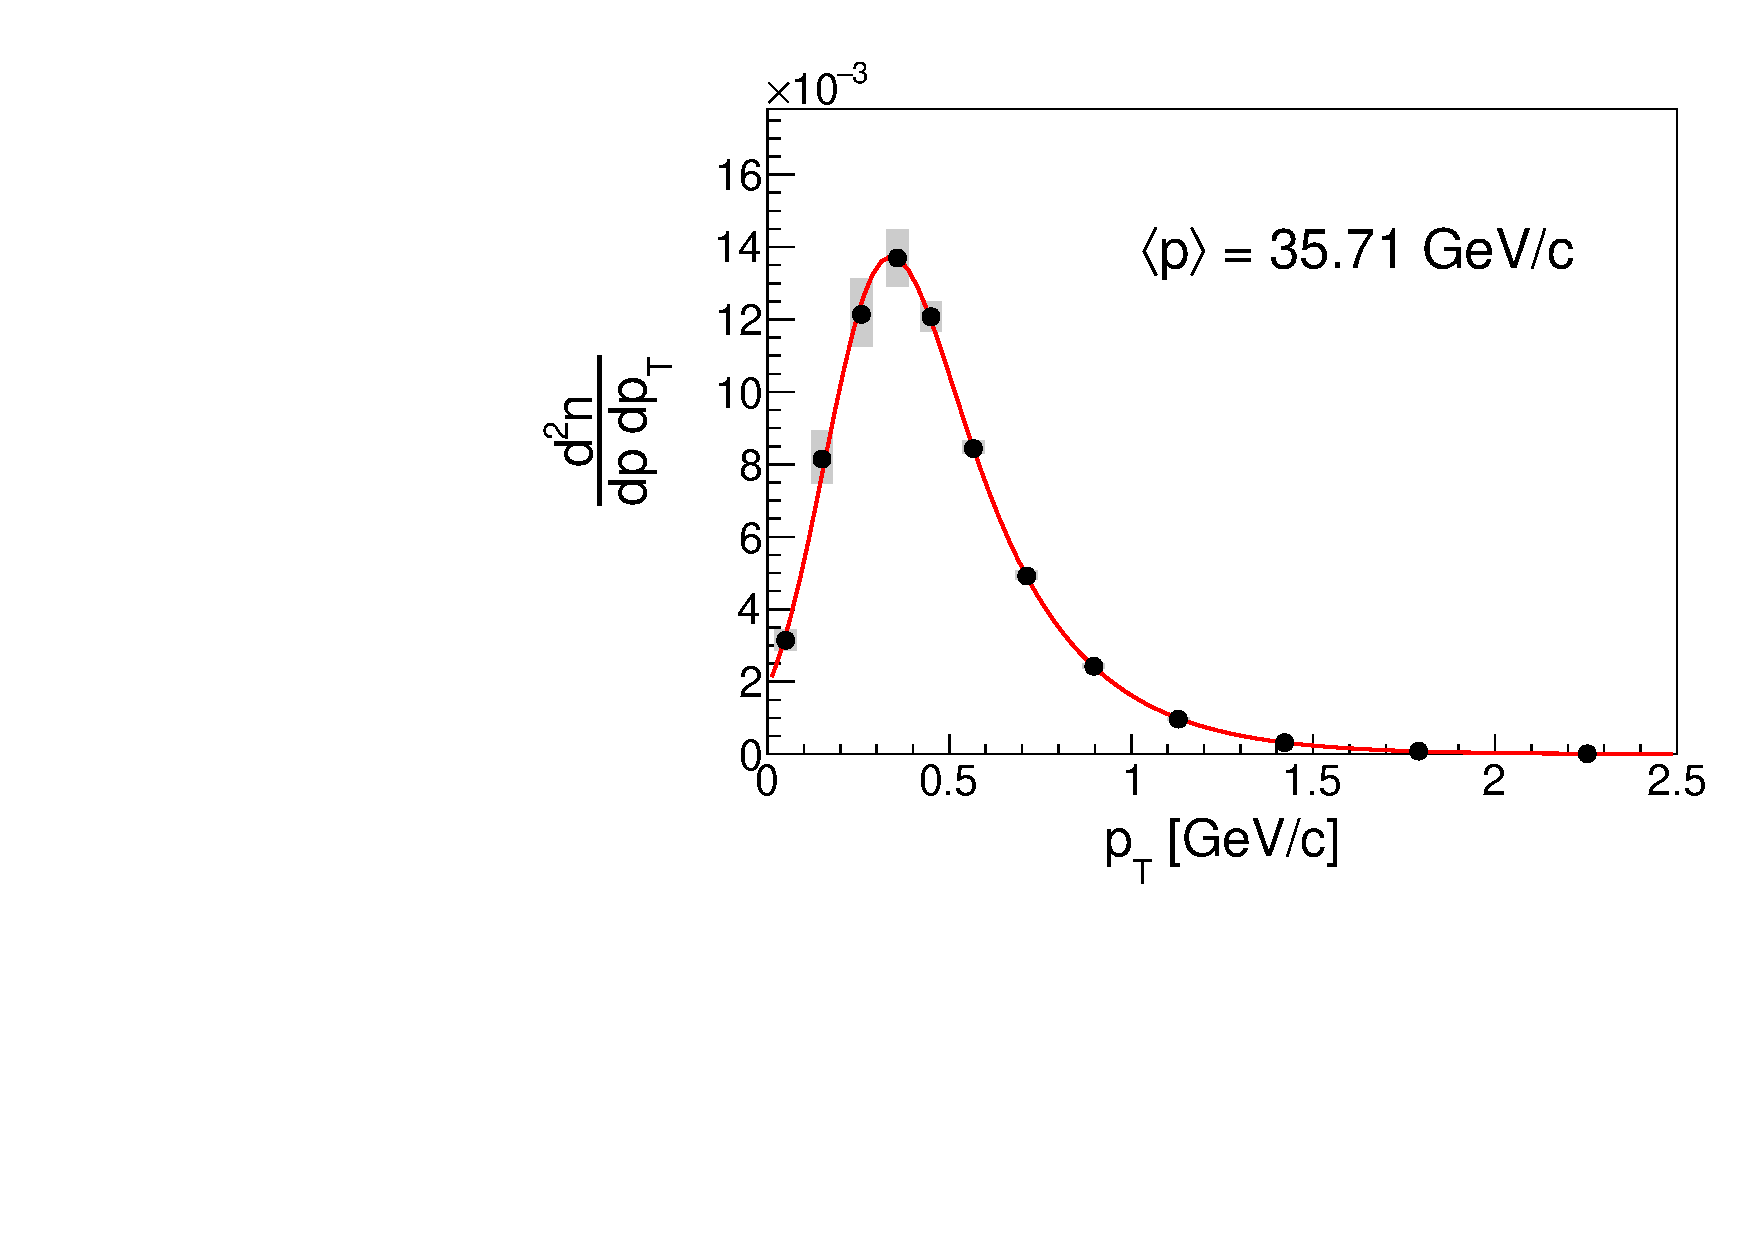
\includegraphics[clip, rviewport=0 0 1 1,width=0.24\textwidth]{spec/spec_pt_158_c0_p1_x26}
  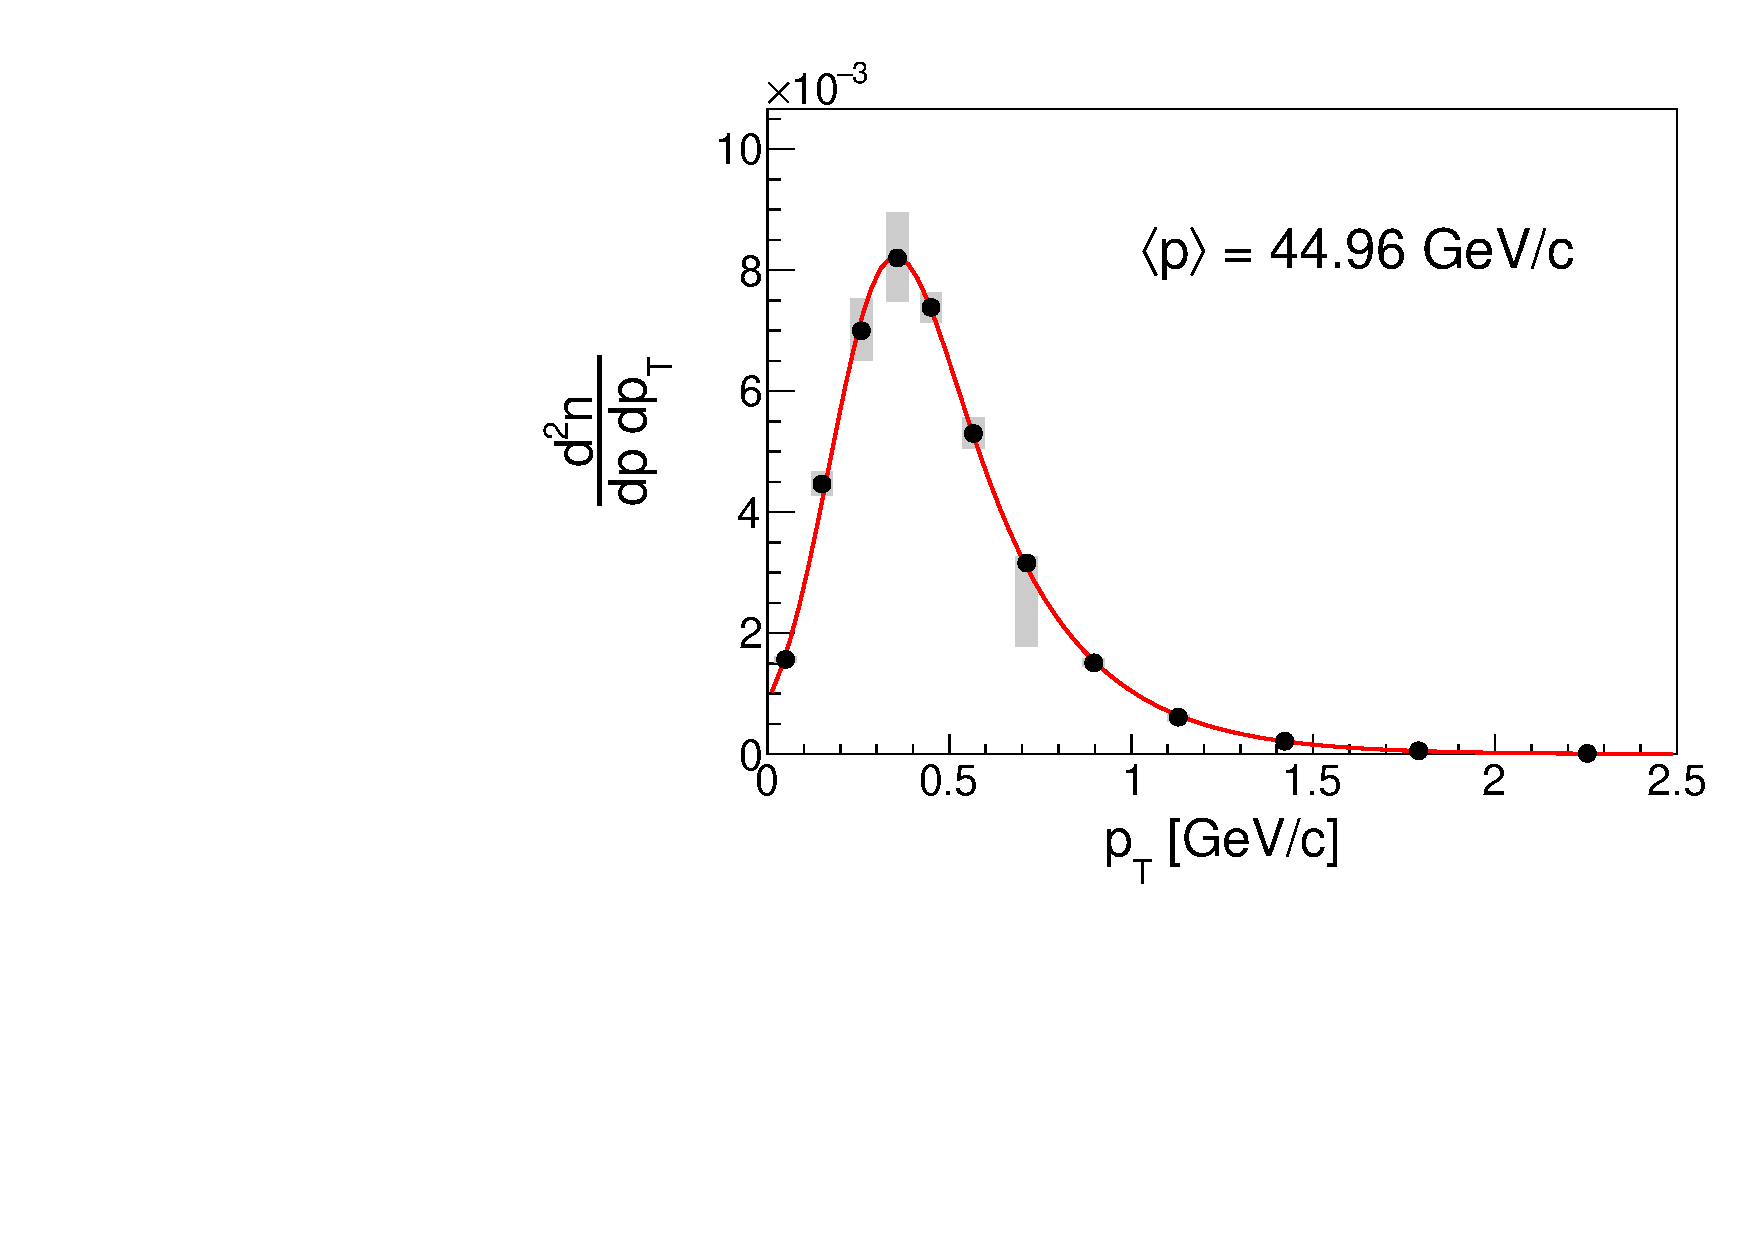
\includegraphics[clip, rviewport=0 0 1 1,width=0.24\textwidth]{spec/spec_pt_158_c0_p1_x27}
  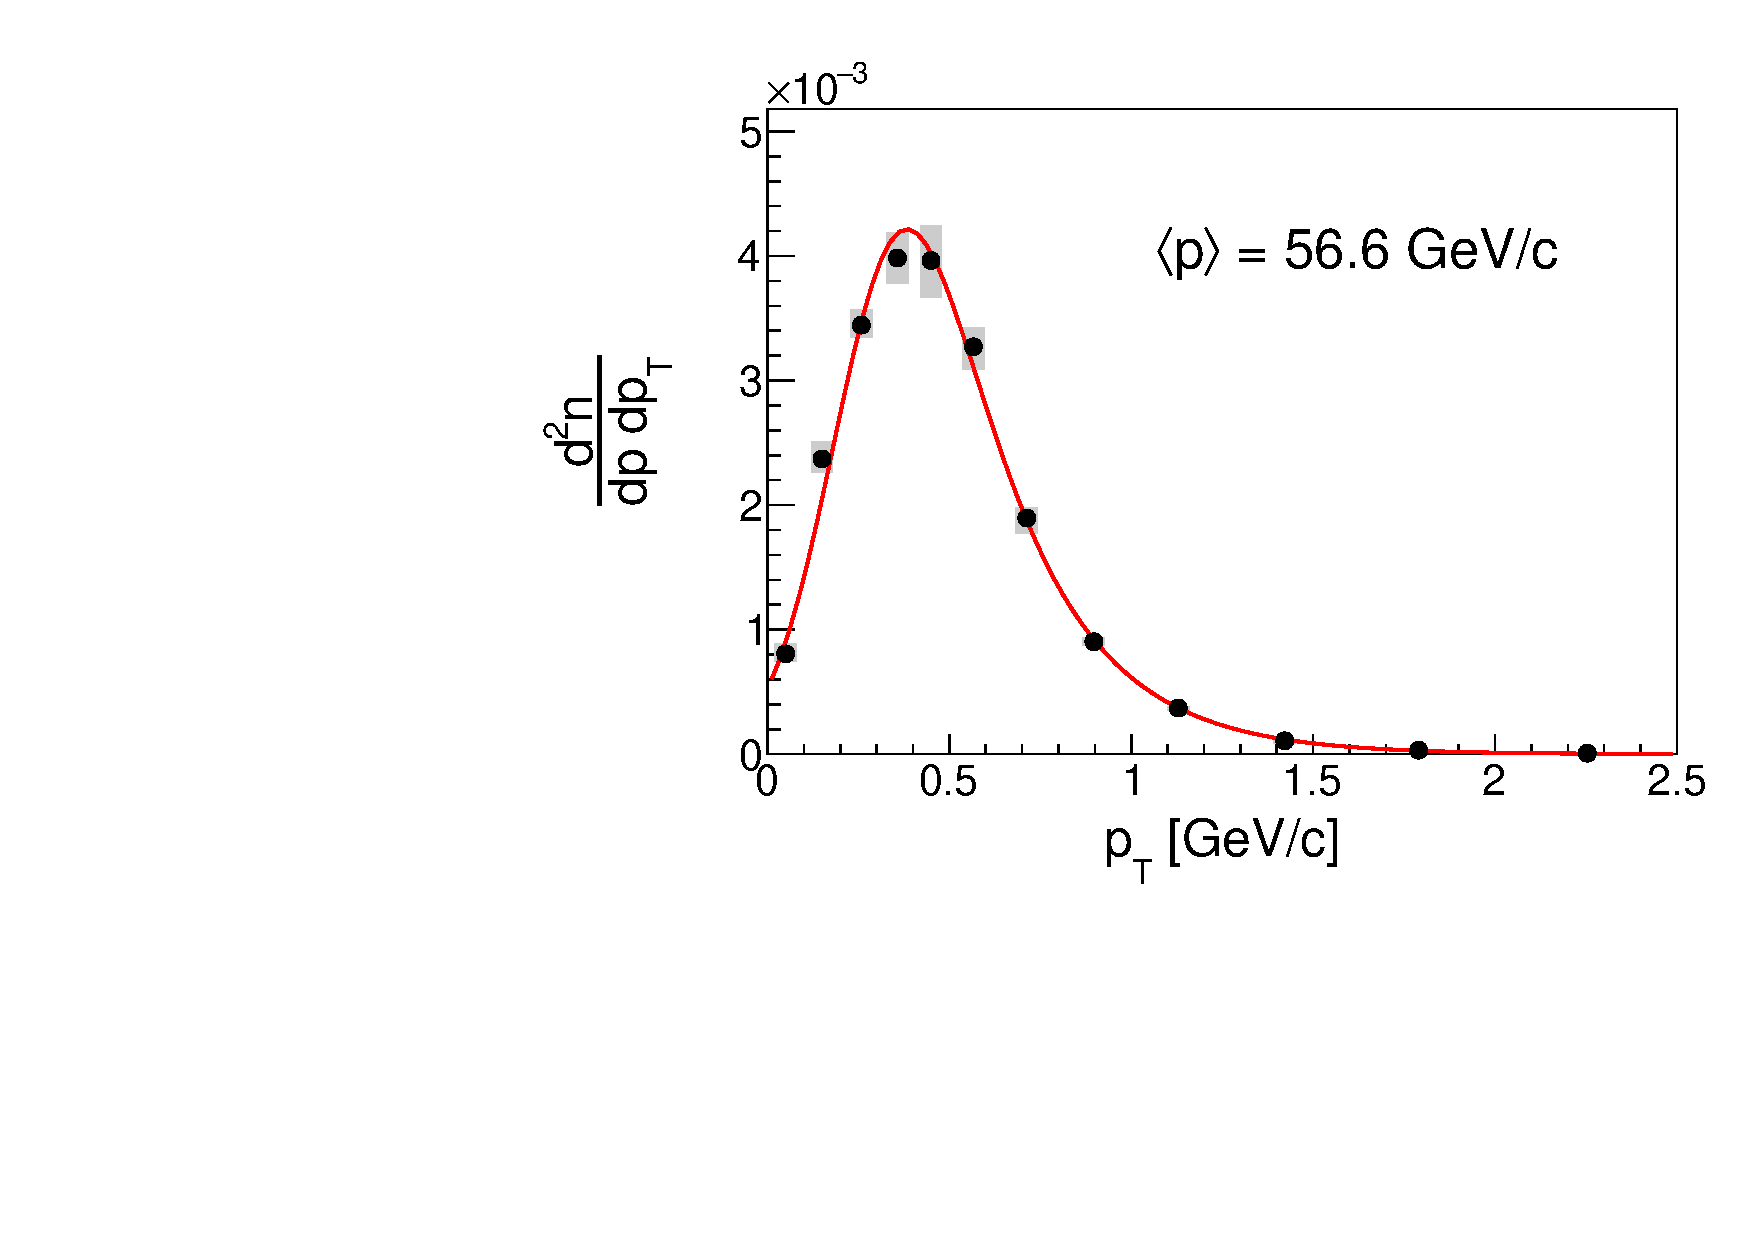
\includegraphics[clip, rviewport=0 0 1 1,width=0.24\textwidth]{spec/spec_pt_158_c0_p1_x28}

  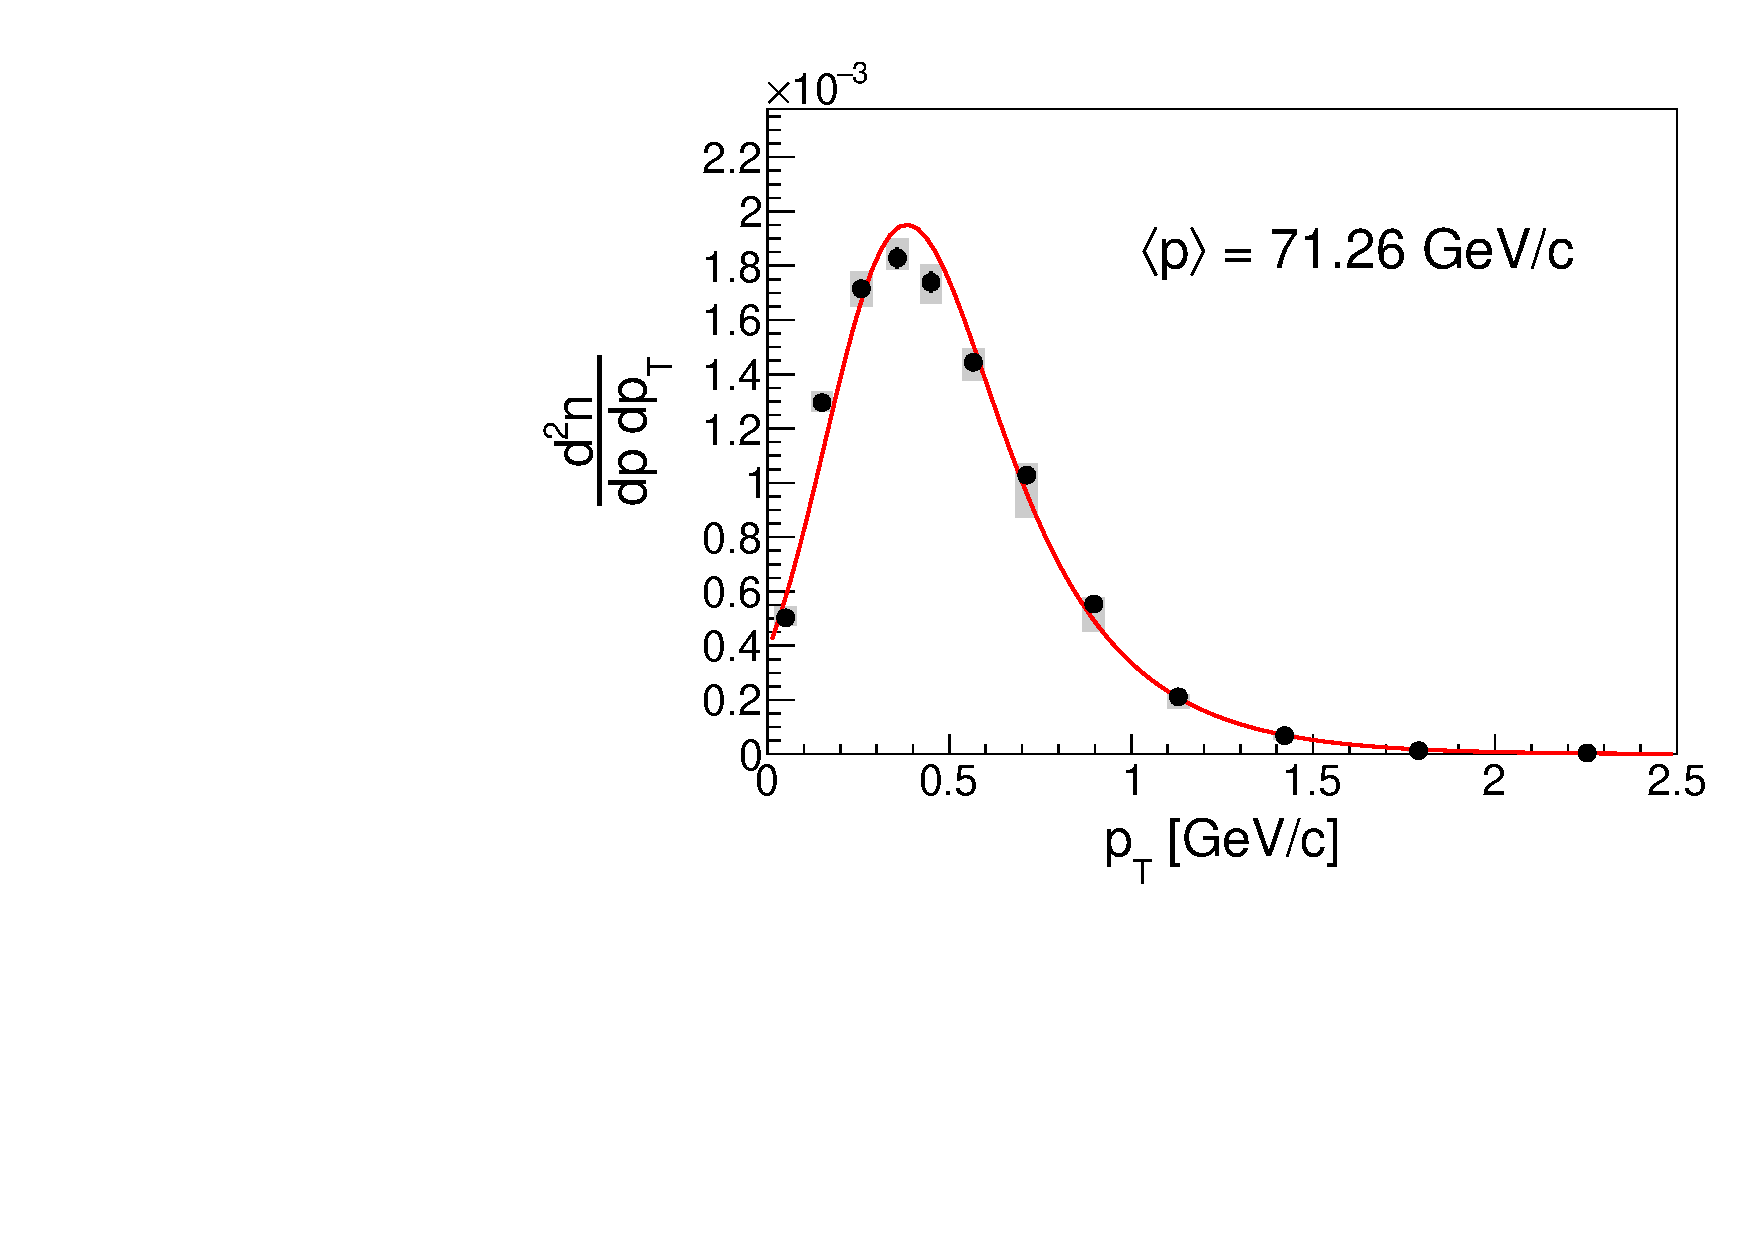
\includegraphics[clip, rviewport=0 0 1 1,width=0.24\textwidth]{spec/spec_pt_158_c0_p1_x29}
  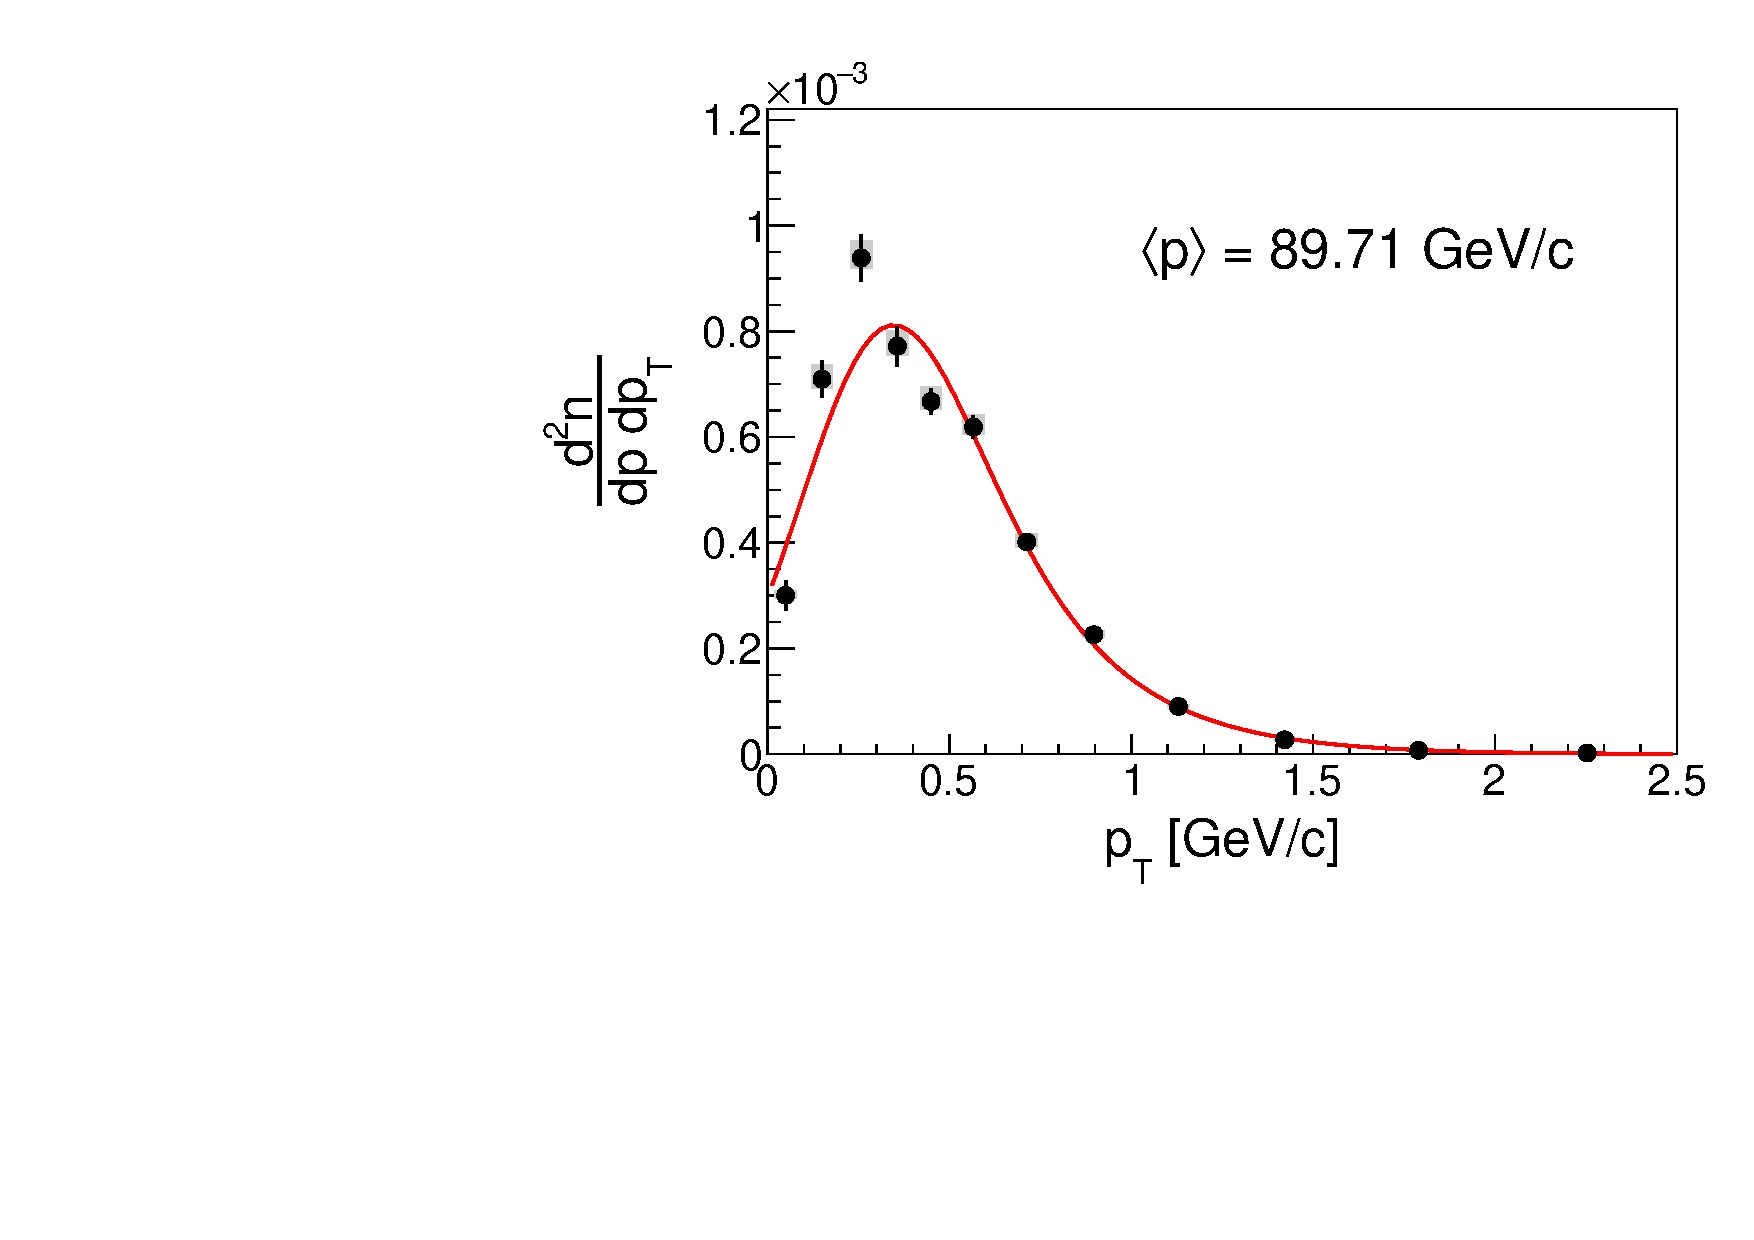
\includegraphics[clip, rviewport=0 0 1 1,width=0.24\textwidth]{spec/spec_pt_158_c0_p1_x30}
  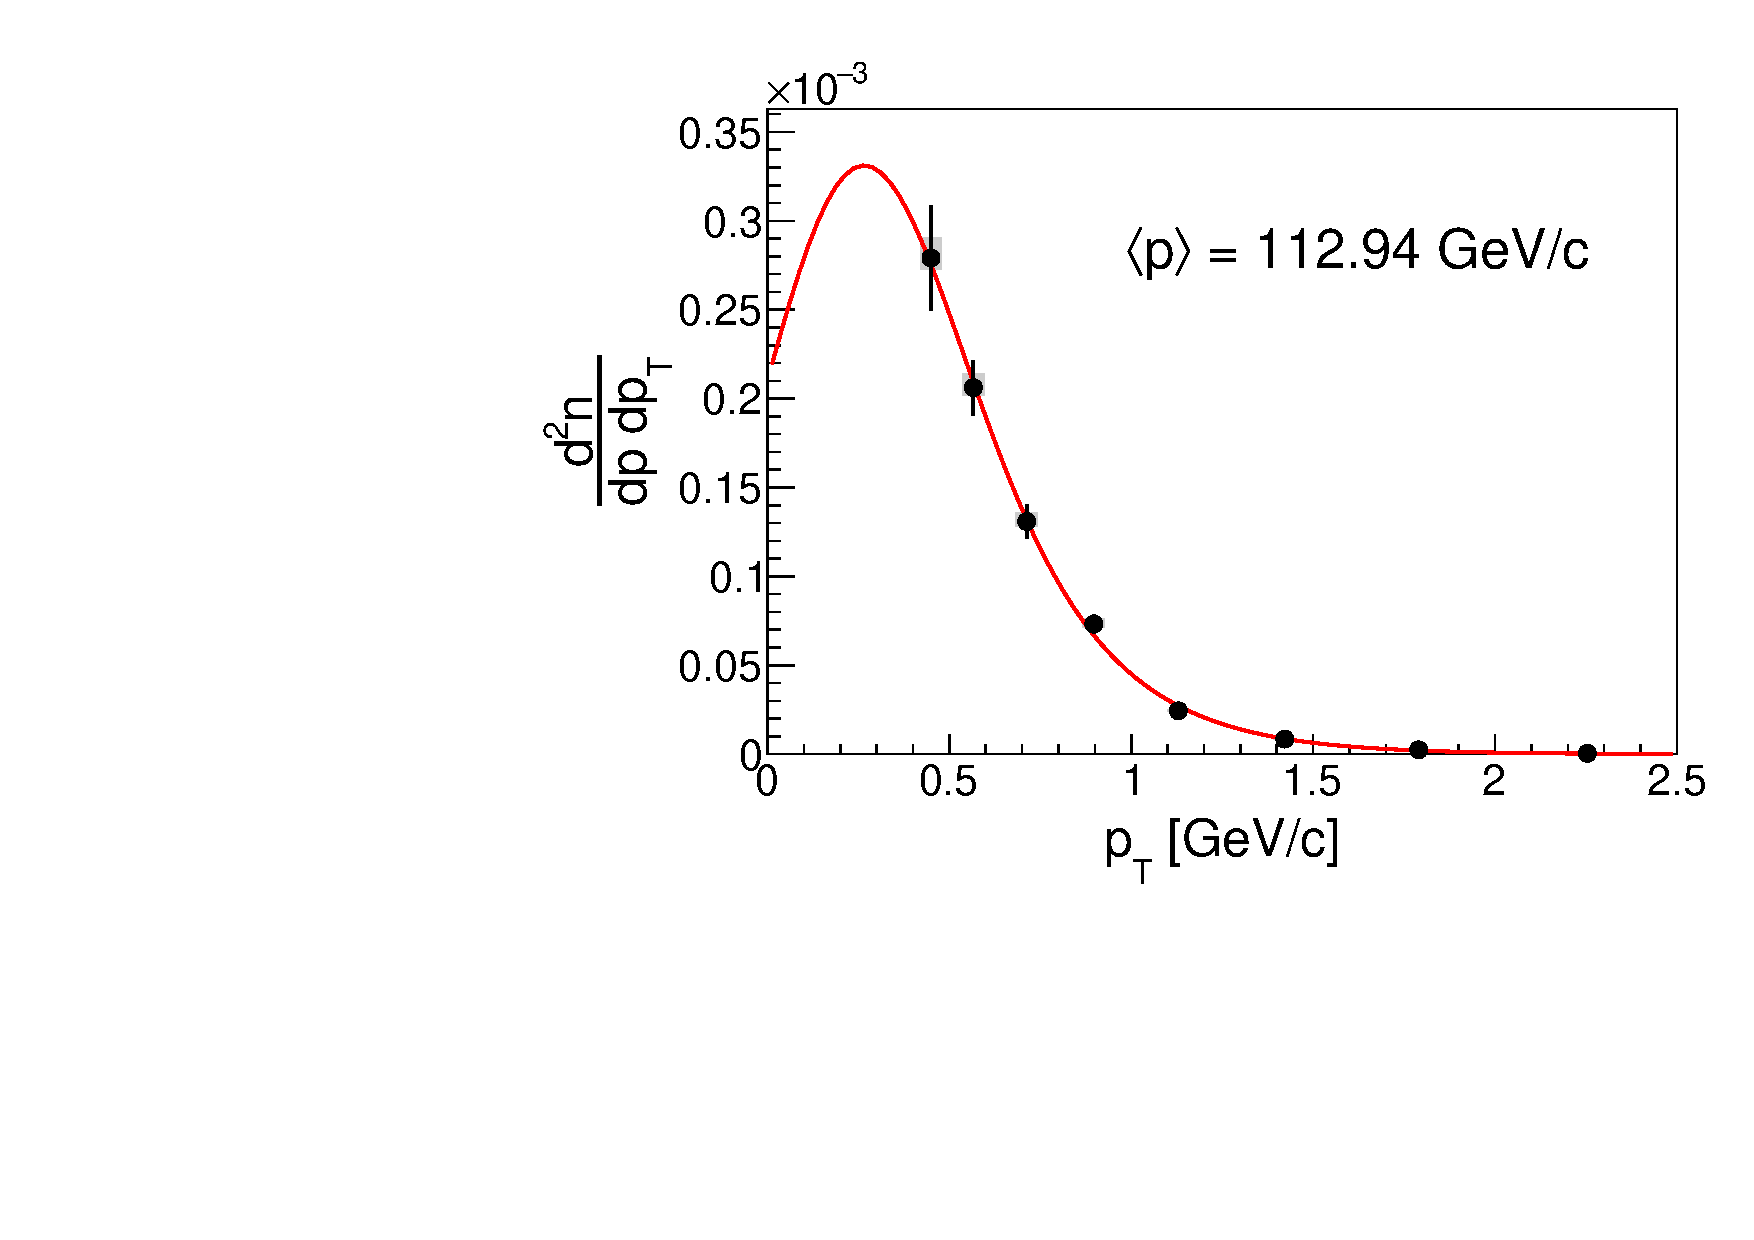
\includegraphics[clip, rviewport=0 0 1 1,width=0.24\textwidth]{spec/spec_pt_158_c0_p1_x31}

  \caption{Double-differential spectra $\frac{\text{d}^2n}{\text{d}\pp\text{d}\pT}$
    of $\pi^+$ for the 158 \GeVc data set. Each plot shows one \pp bins and the value
    of $\langle\pp\rangle$ is indicated inside it. The black lines show the statistical
    uncertainties, while the gray bands show the systematic ones.}
  \label{fig:hadron:spec:dedx:all158:c0p1}
  \begin{center}
    Source: By the author. 
  \end{center}
\end{figure}

%%%%%%%%%% SPEC PT ALL DEDX %%%%%%%%%%%%%%
\begin{figure}[!ht]
  \centering

  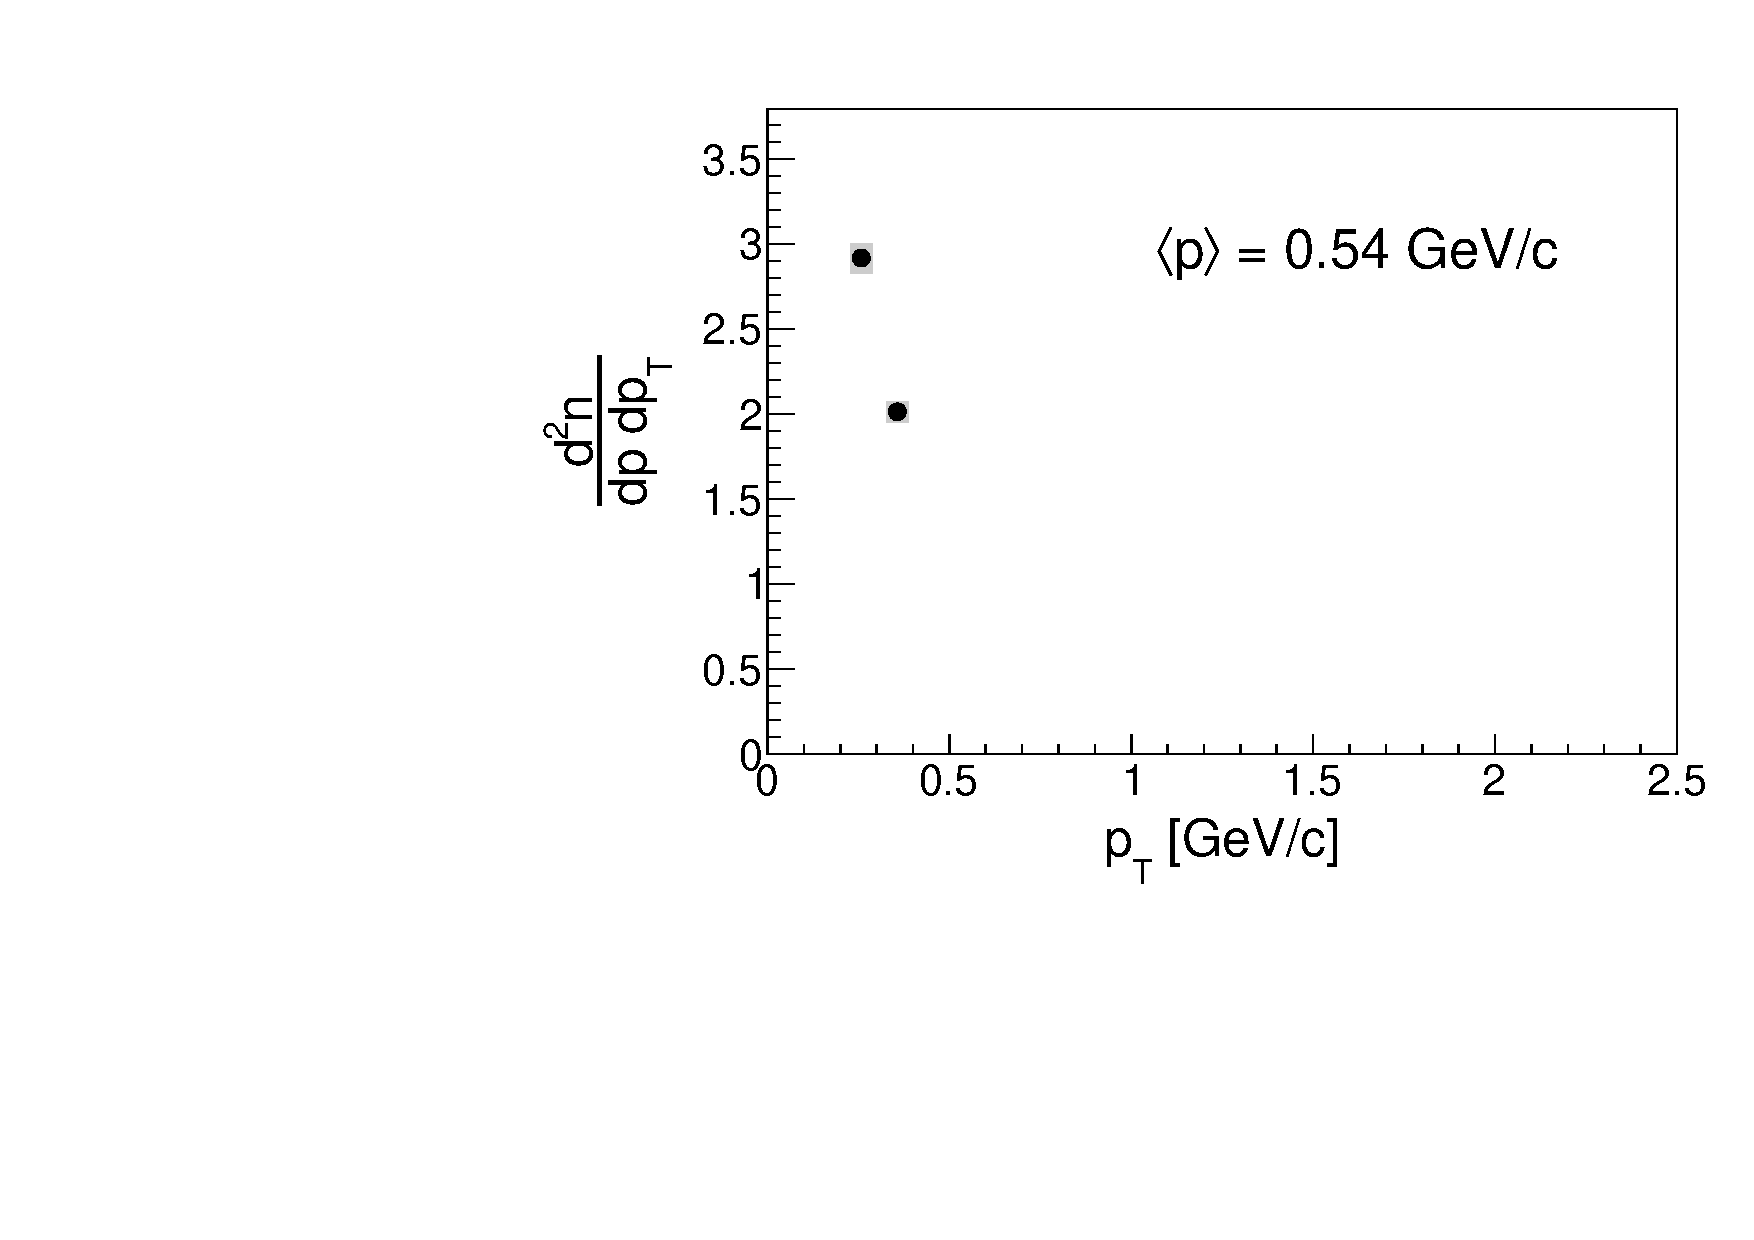
\includegraphics[clip, rviewport=0 0 1 1,width=0.24\textwidth]{spec/spec_pt_158_c1_p1_x7}
  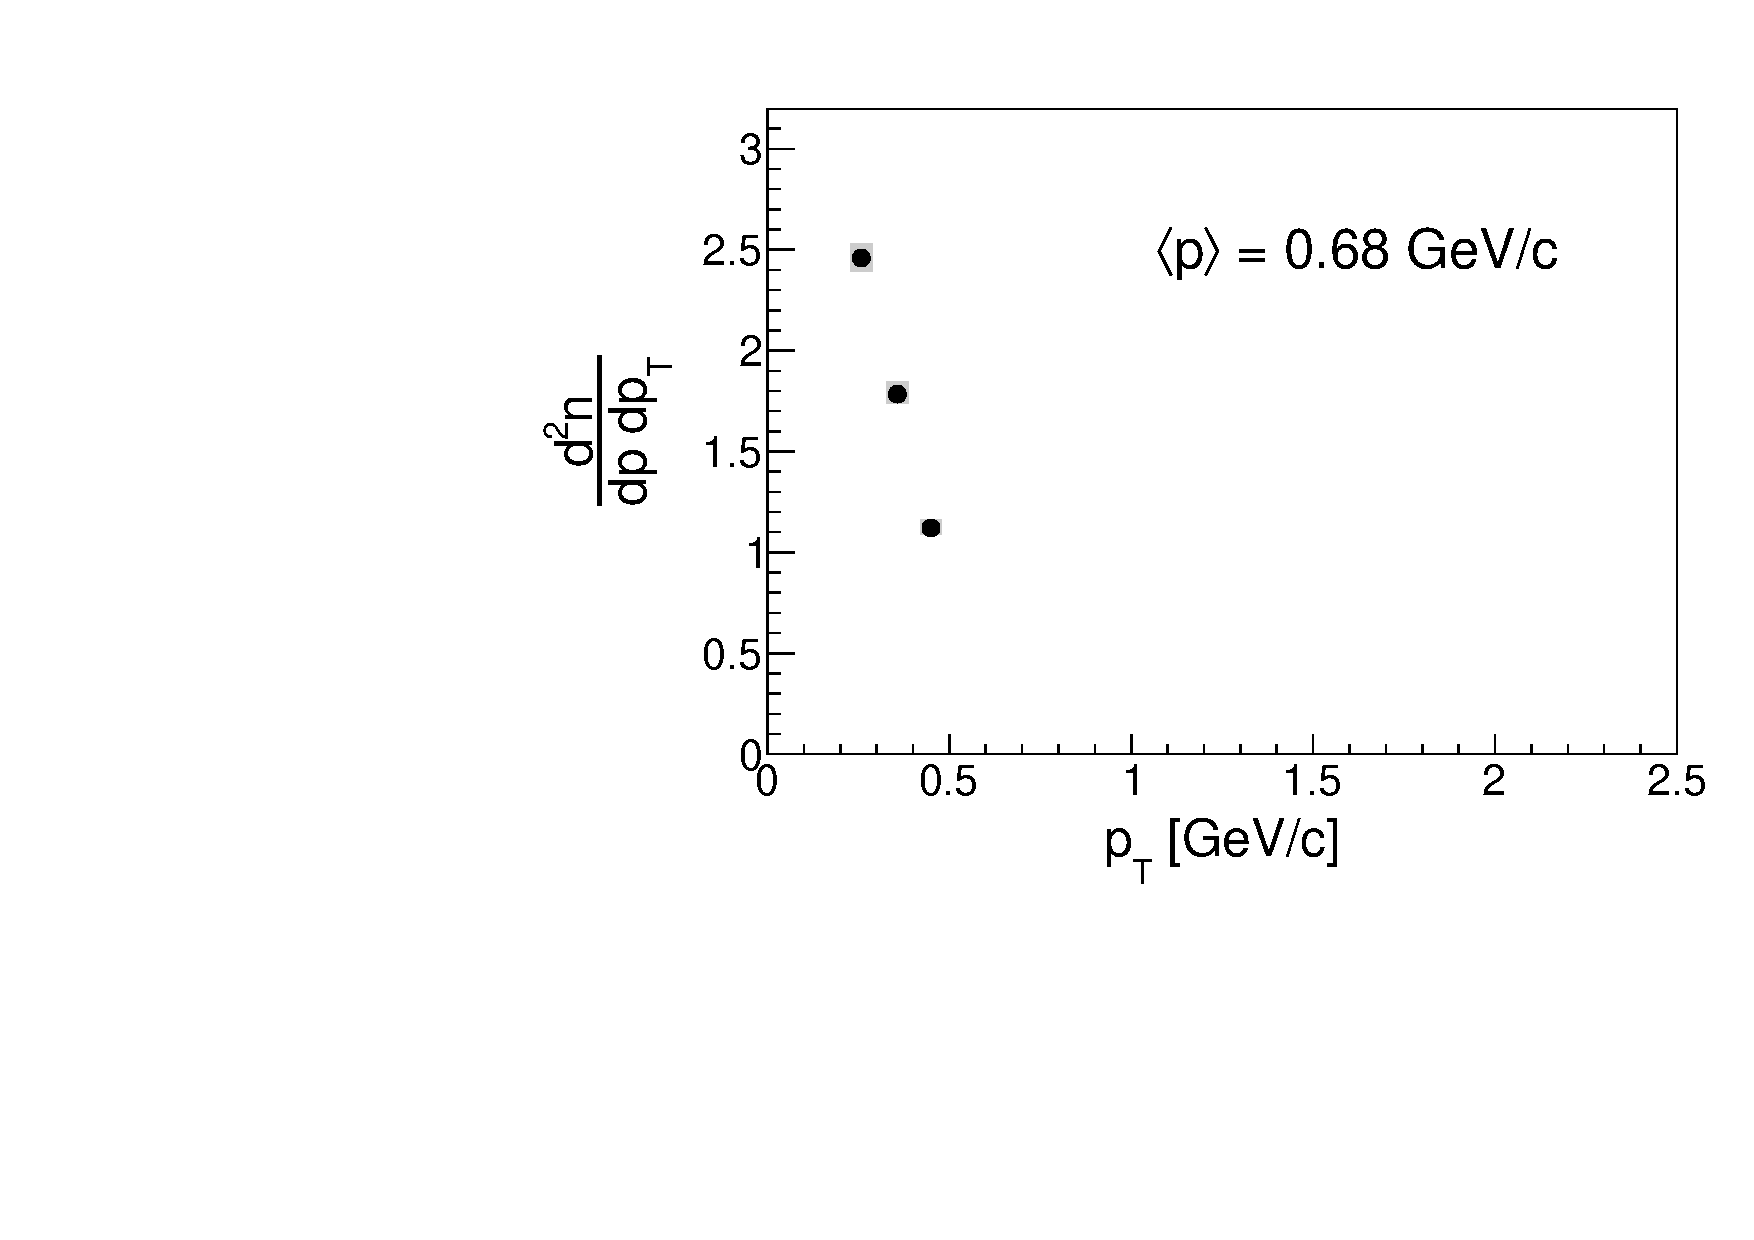
\includegraphics[clip, rviewport=0 0 1 1,width=0.24\textwidth]{spec/spec_pt_158_c1_p1_x8}
  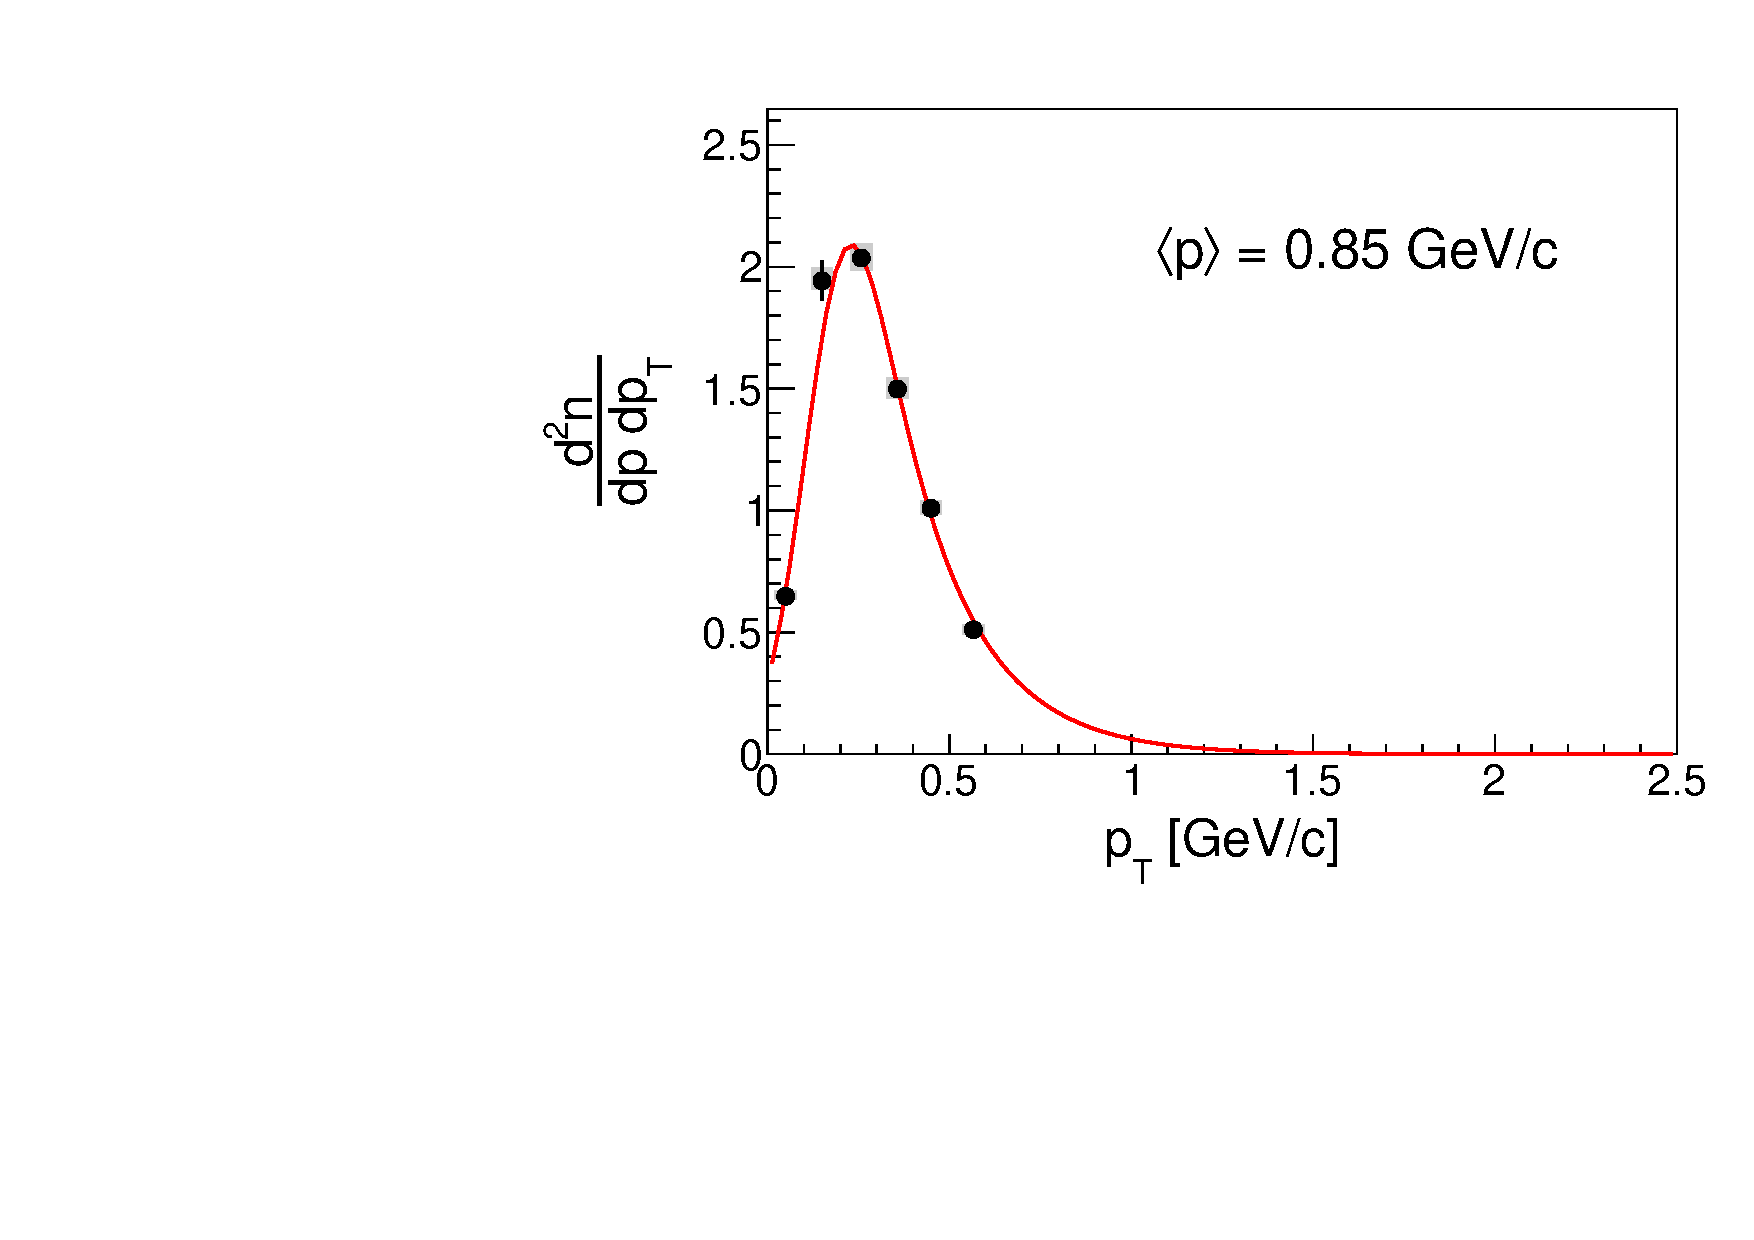
\includegraphics[clip, rviewport=0 0 1 1,width=0.24\textwidth]{spec/spec_pt_158_c1_p1_x9}
  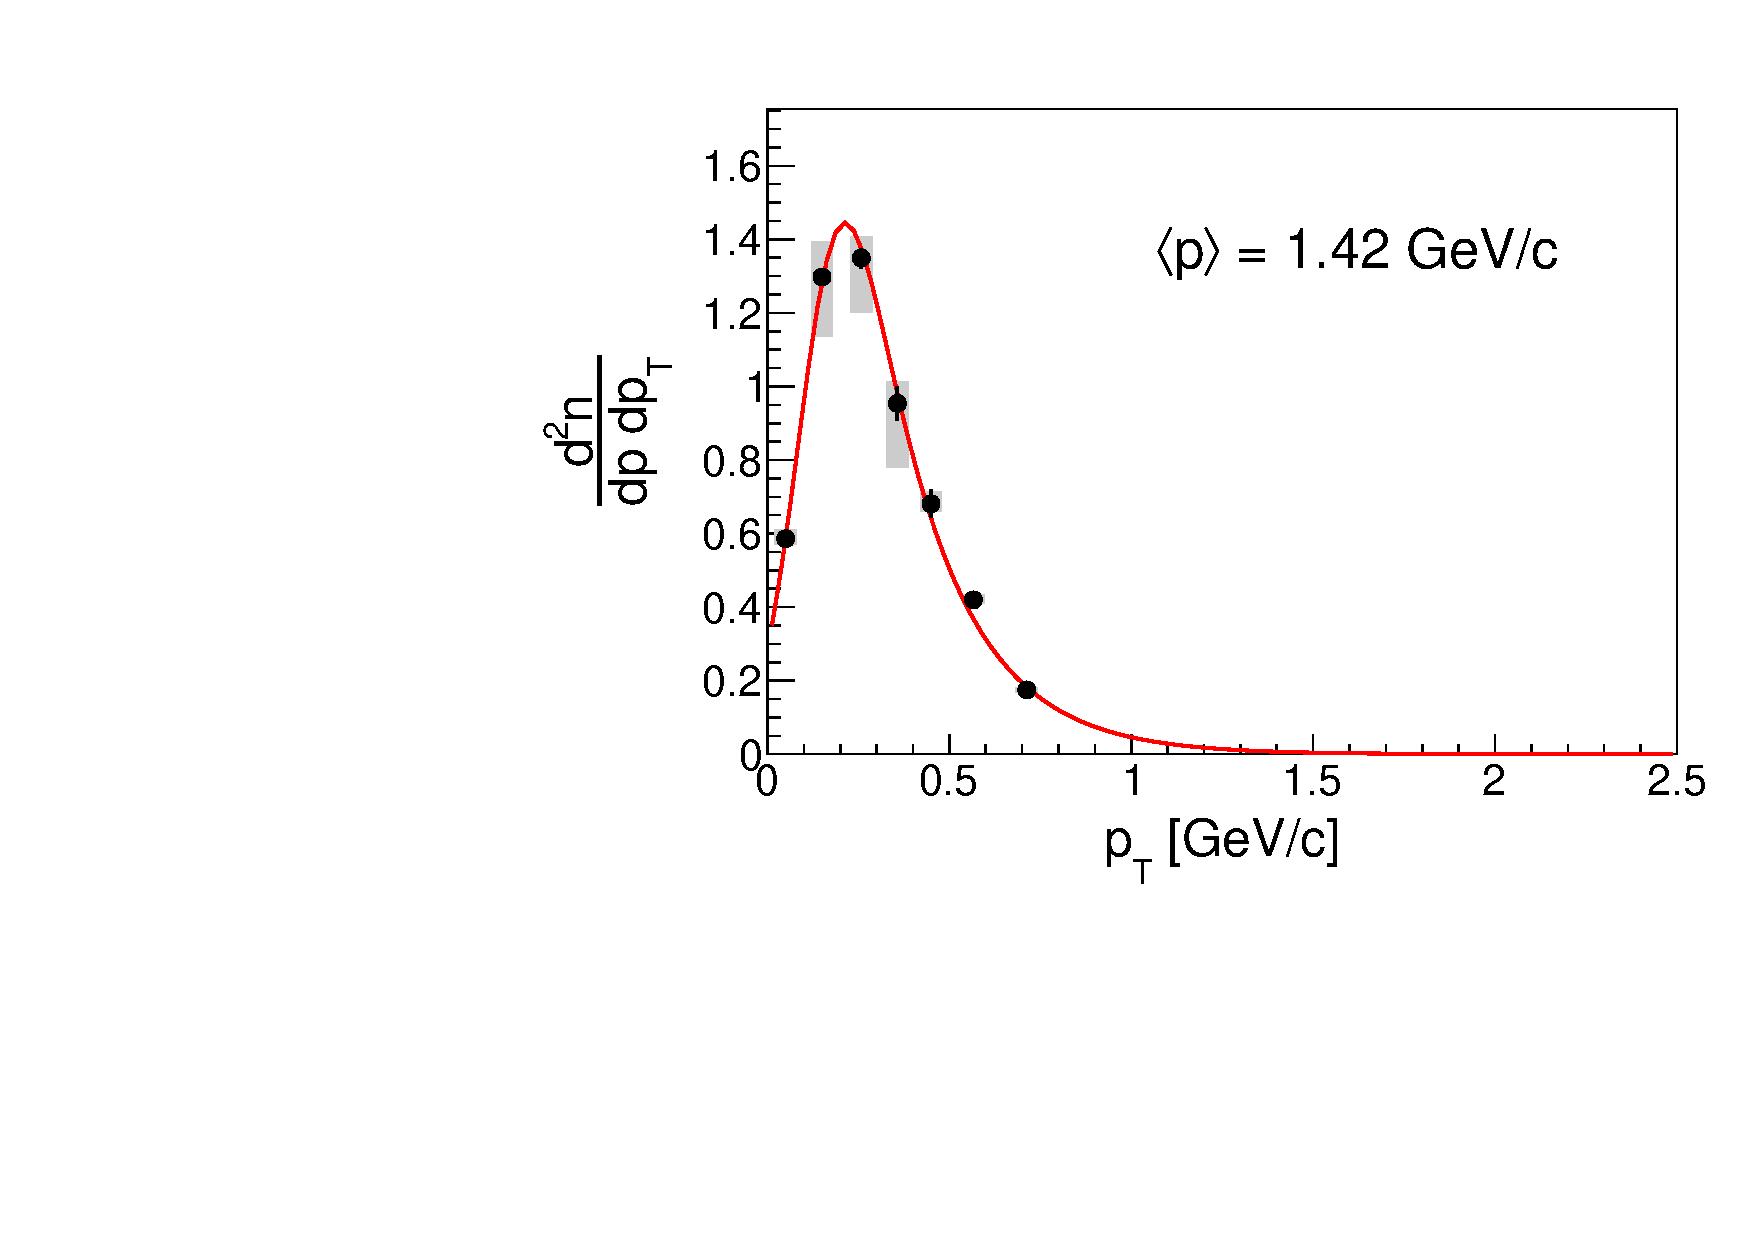
\includegraphics[clip, rviewport=0 0 1 1,width=0.24\textwidth]{spec/spec_pt_158_c1_p1_x11}

  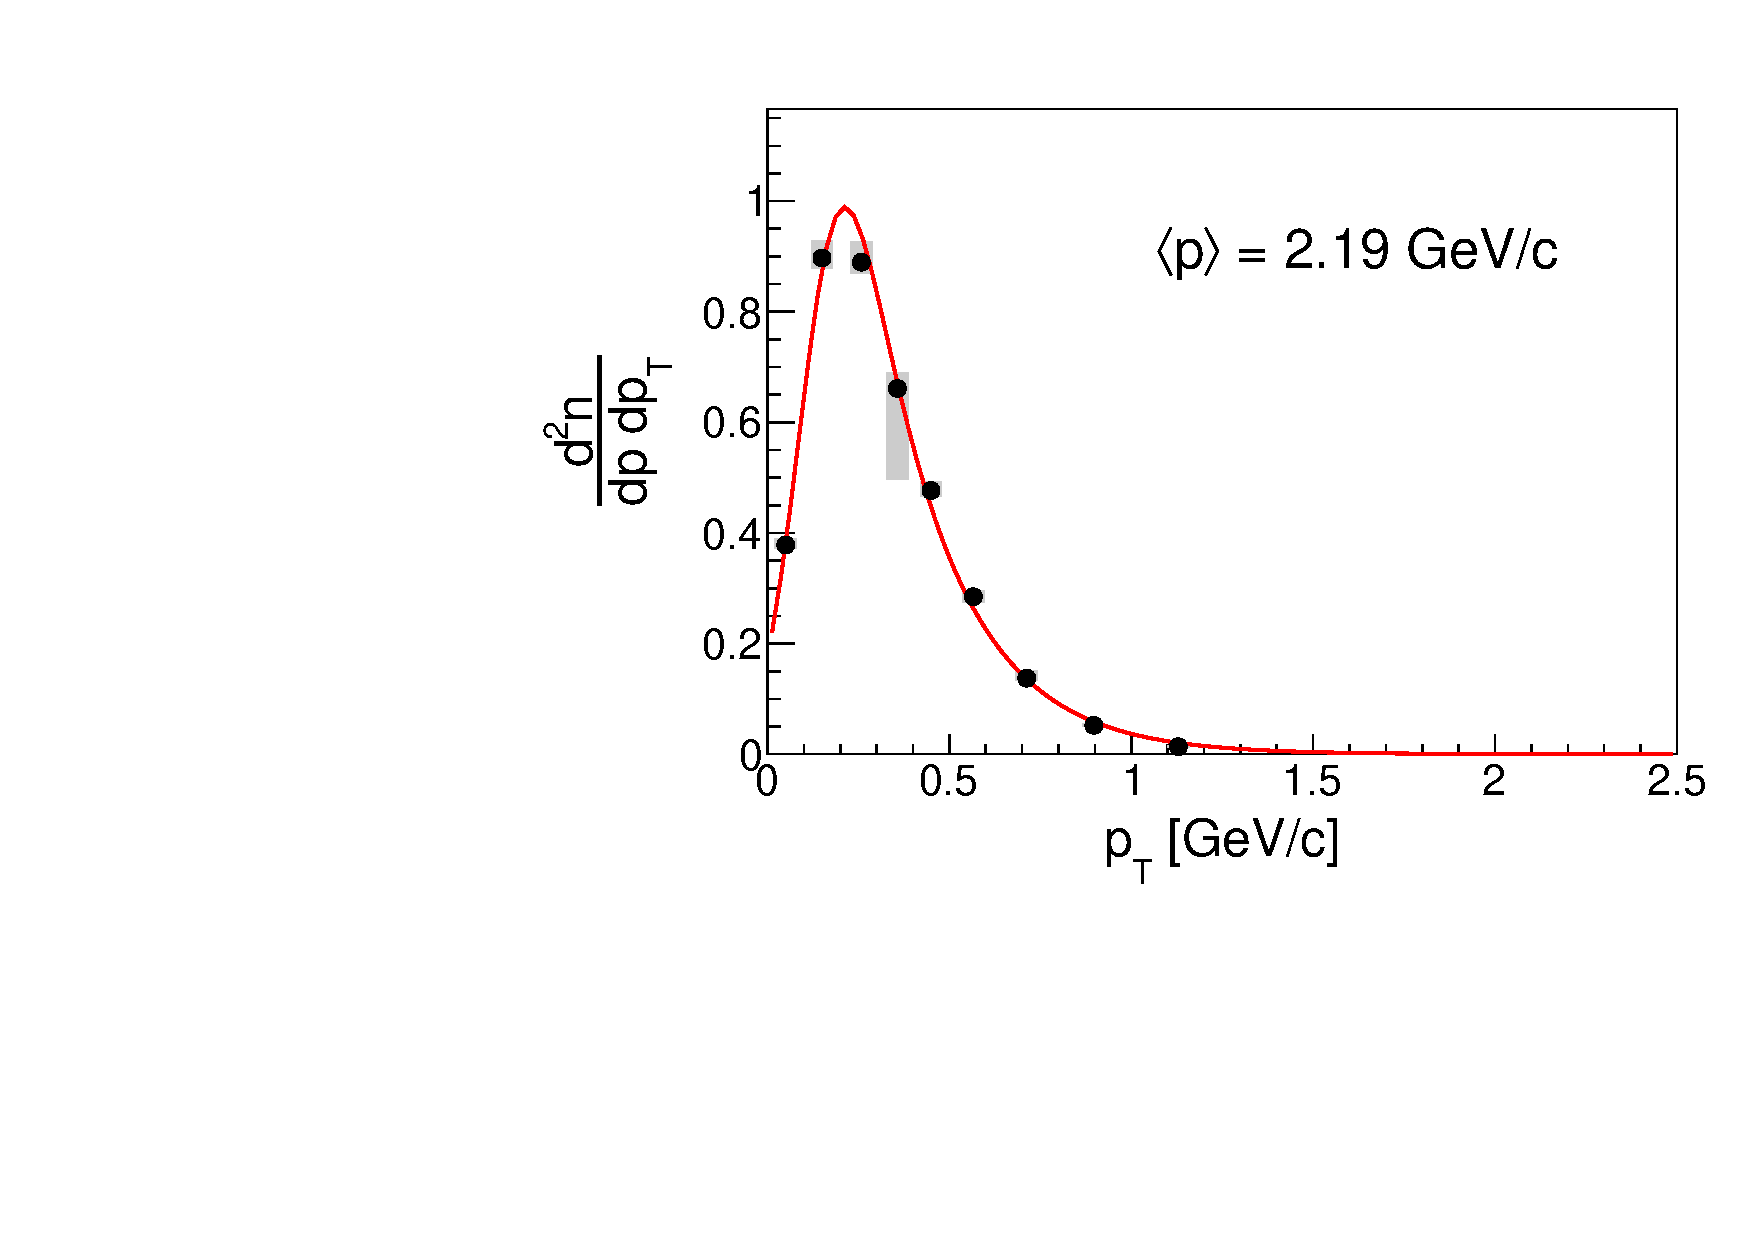
\includegraphics[clip, rviewport=0 0 1 1,width=0.24\textwidth]{spec/spec_pt_158_c1_p1_x13}
  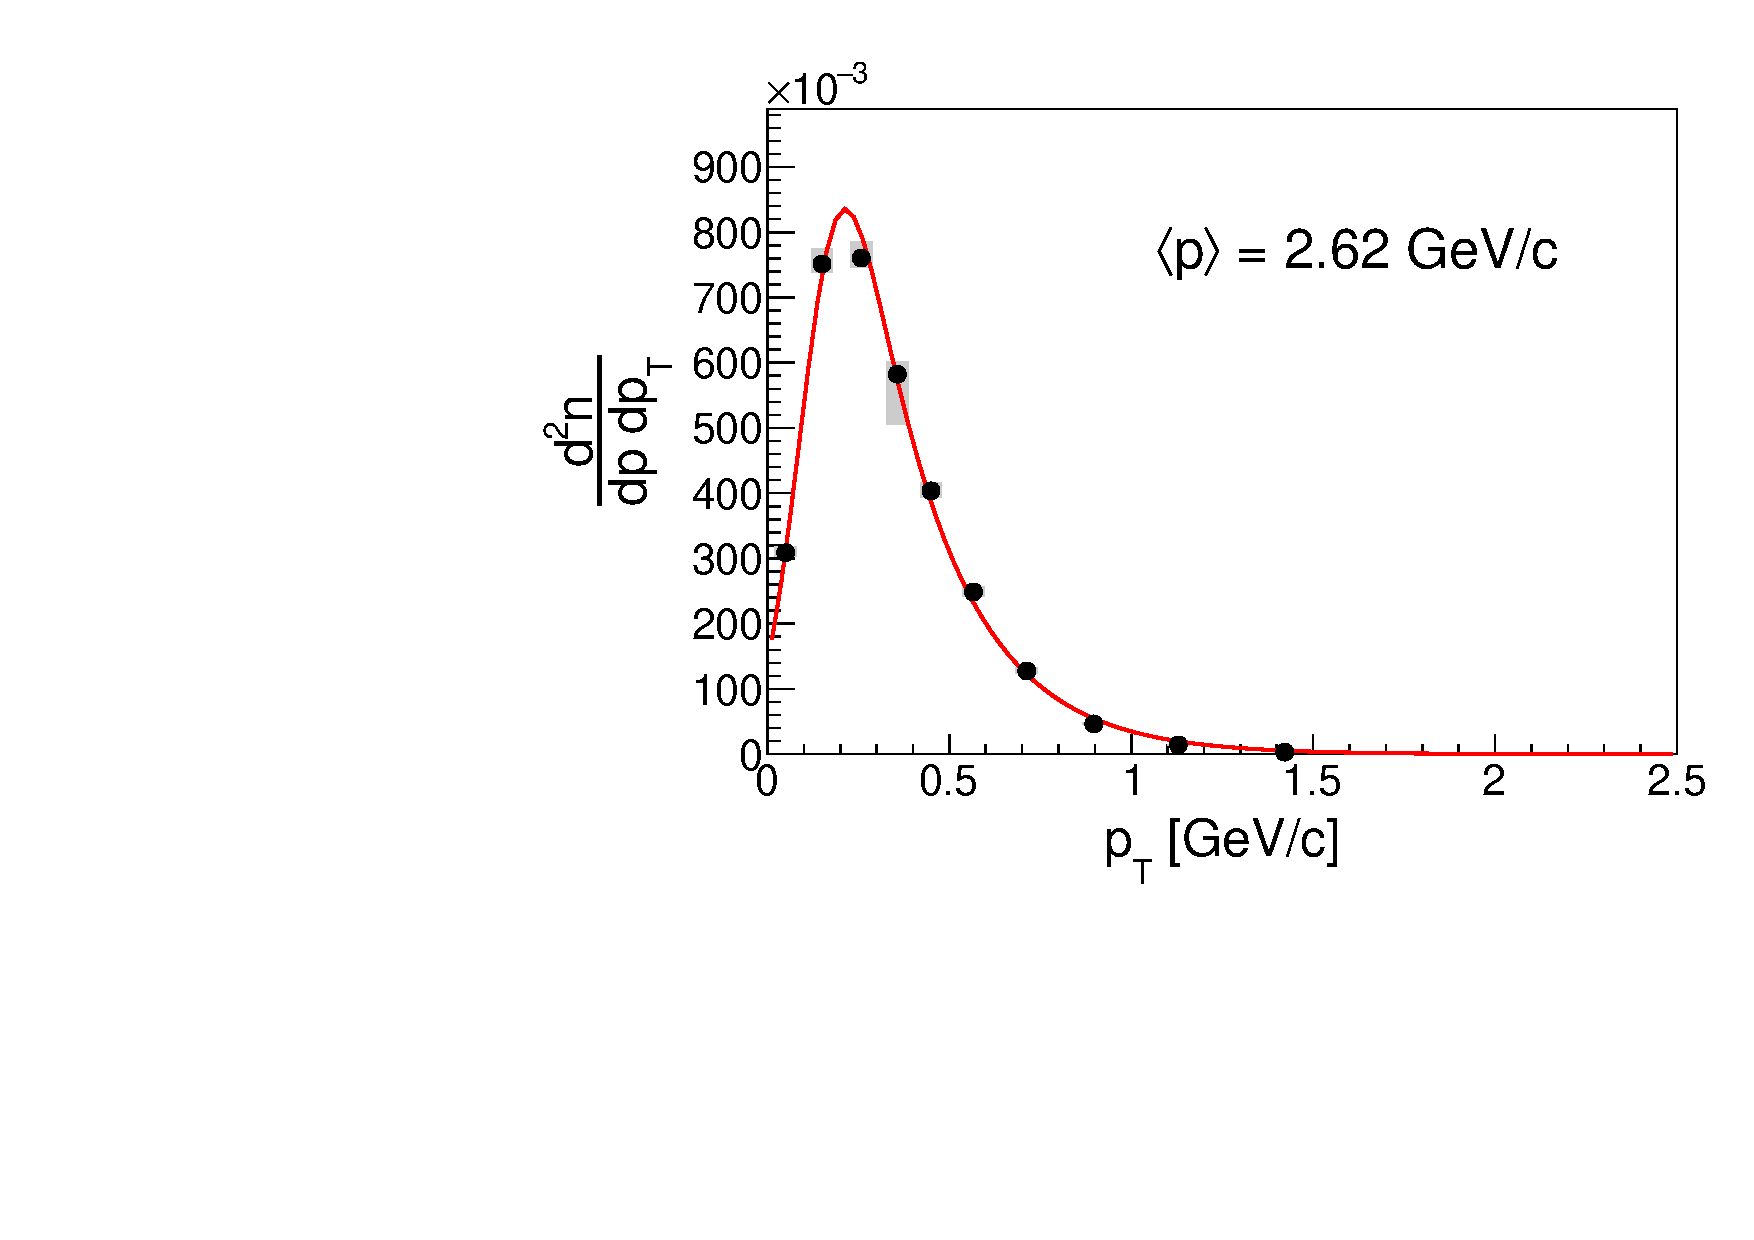
\includegraphics[clip, rviewport=0 0 1 1,width=0.24\textwidth]{spec/spec_pt_158_c1_p1_x14}
  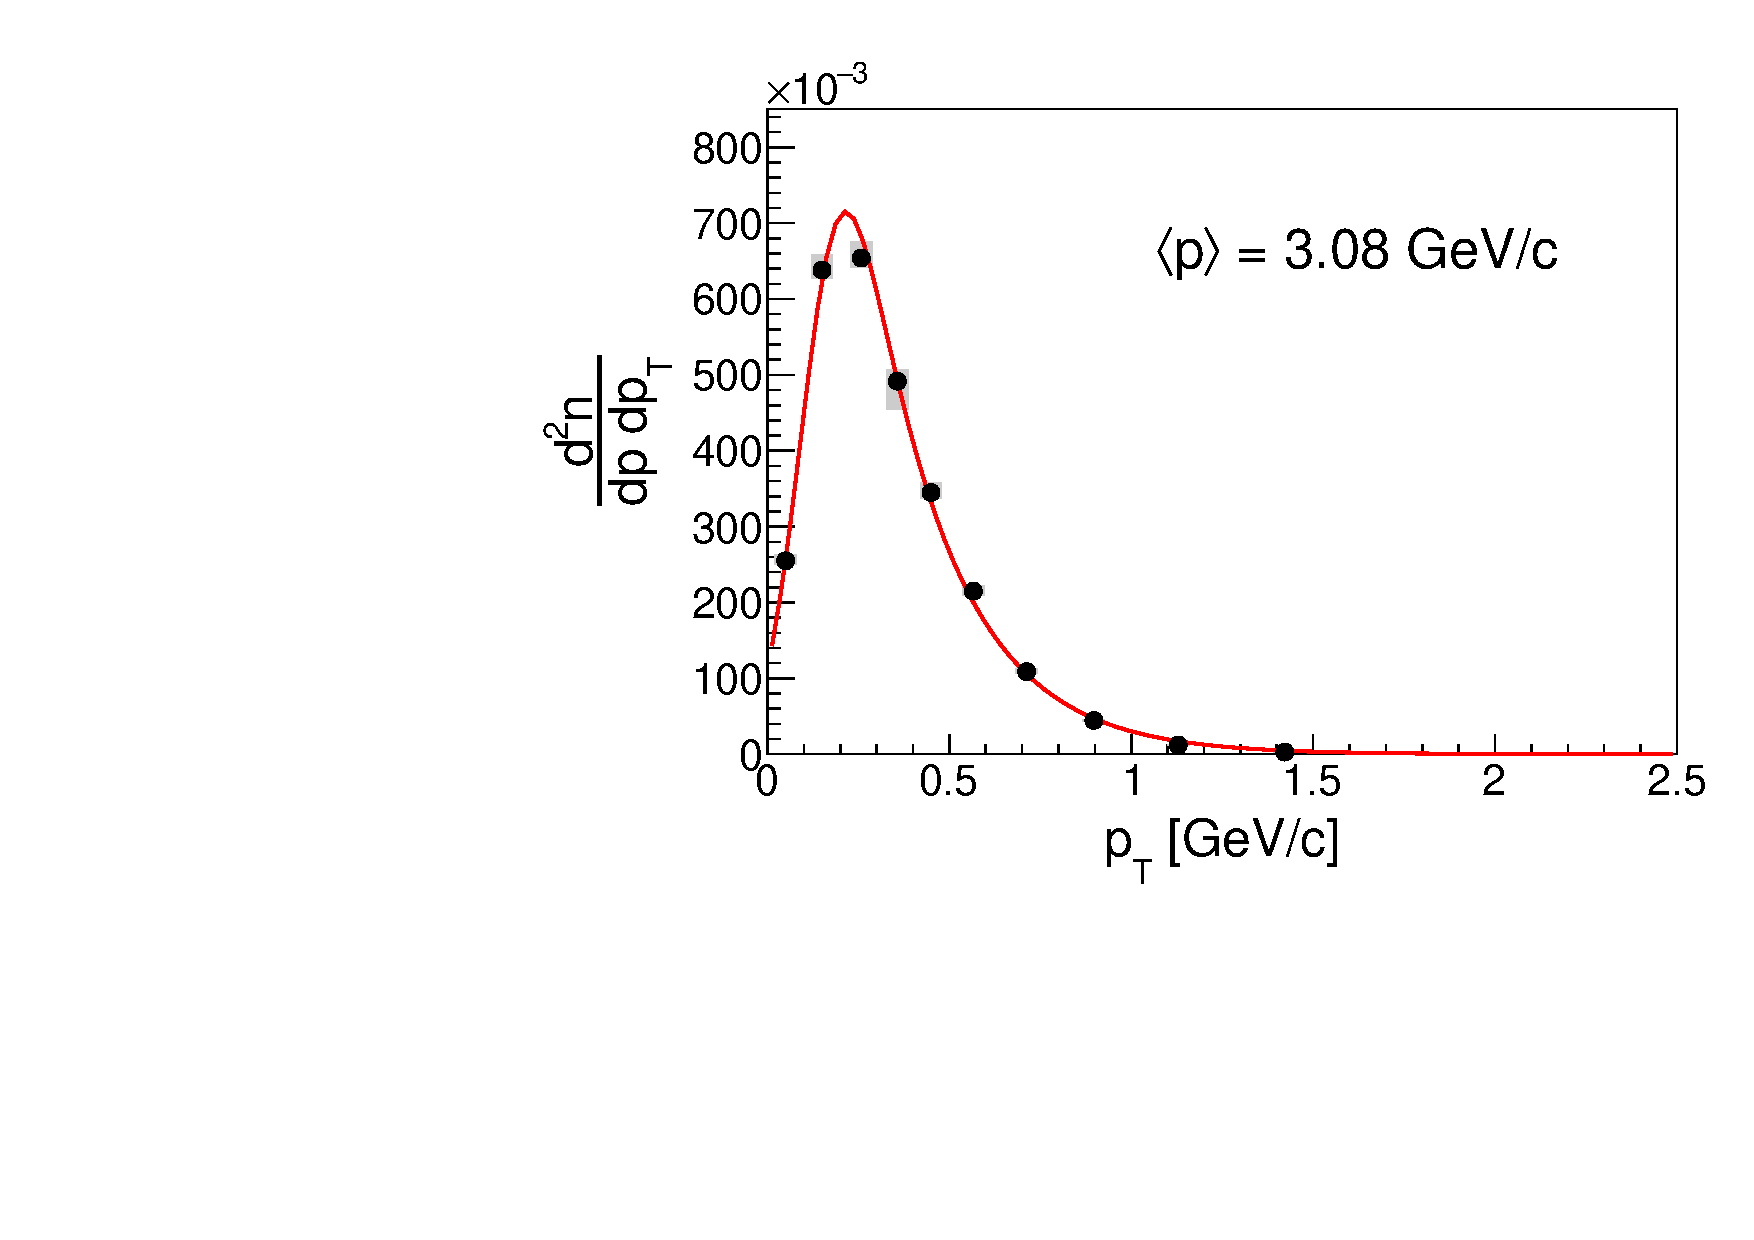
\includegraphics[clip, rviewport=0 0 1 1,width=0.24\textwidth]{spec/spec_pt_158_c1_p1_x15}
  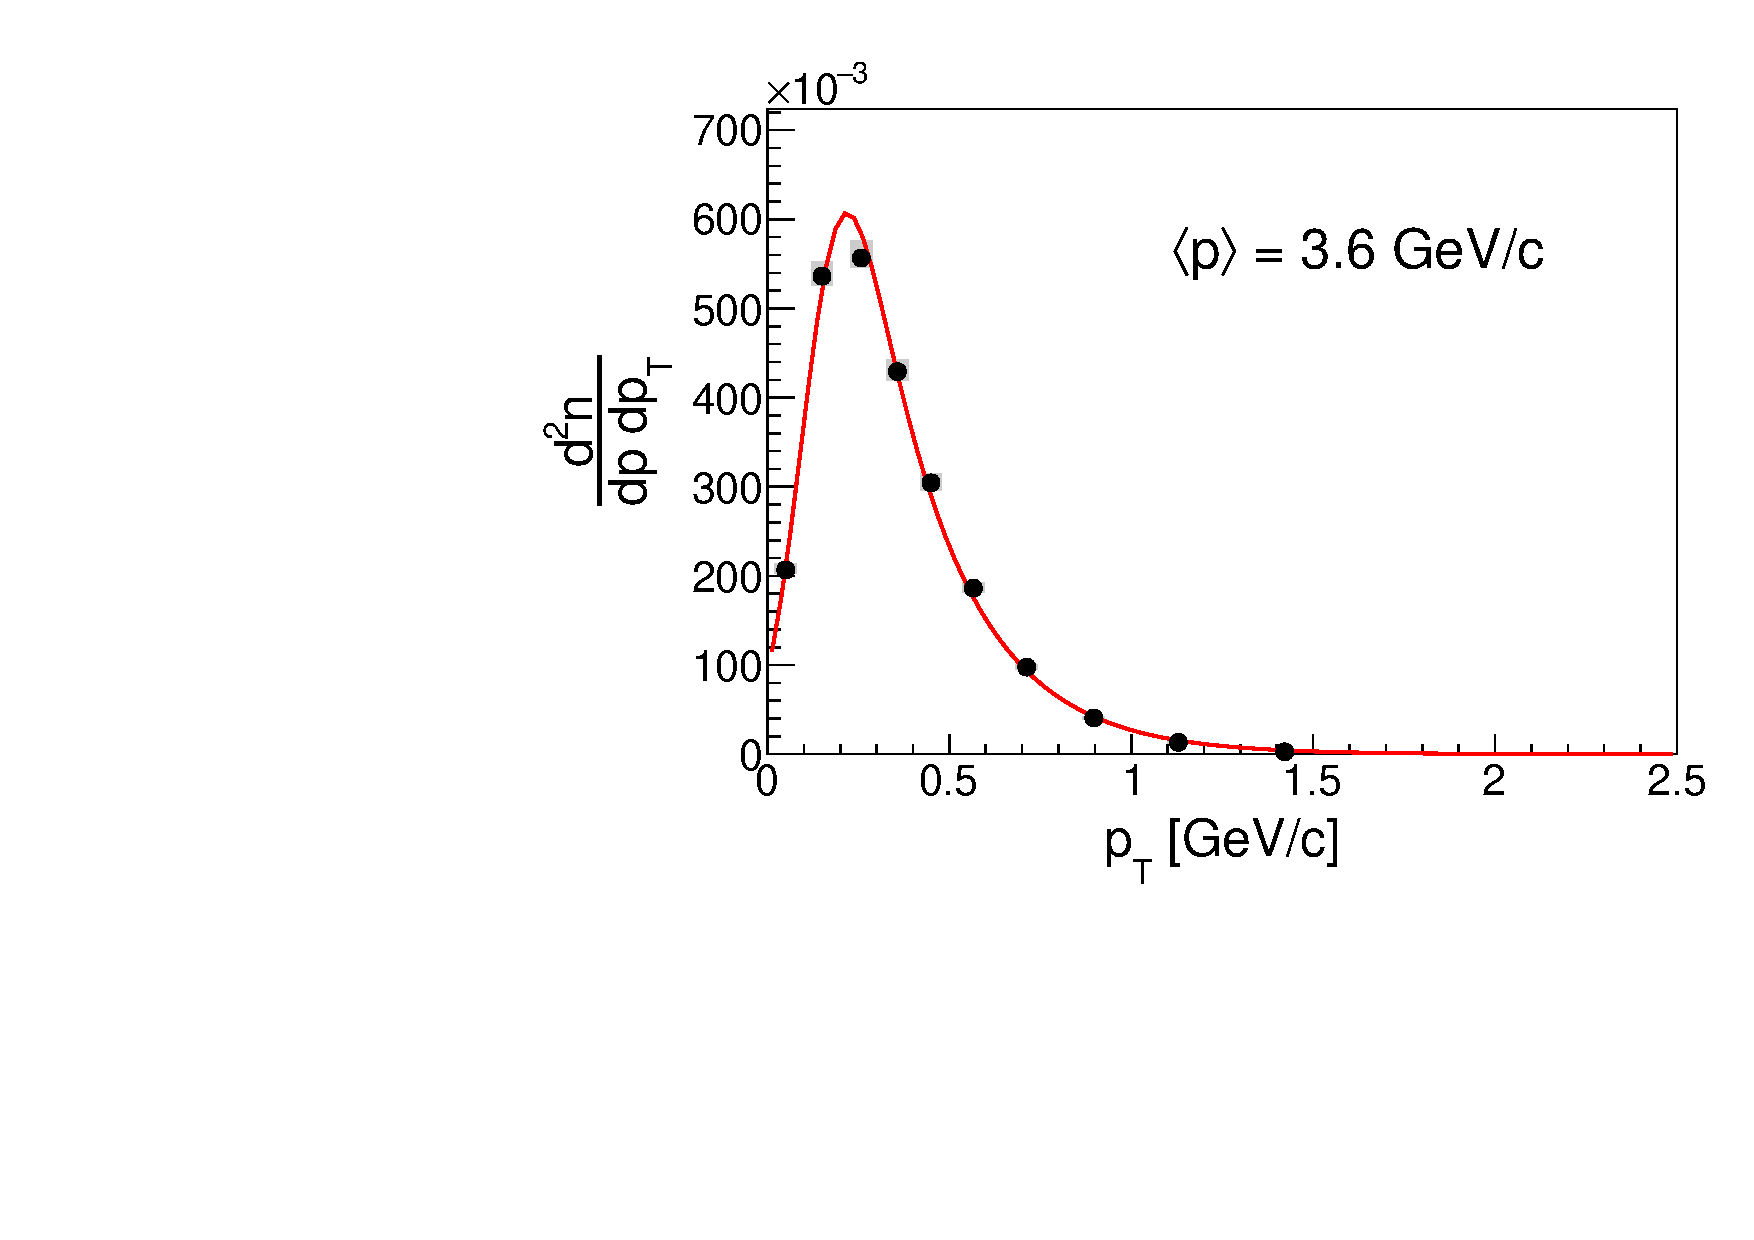
\includegraphics[clip, rviewport=0 0 1 1,width=0.24\textwidth]{spec/spec_pt_158_c1_p1_x16}

  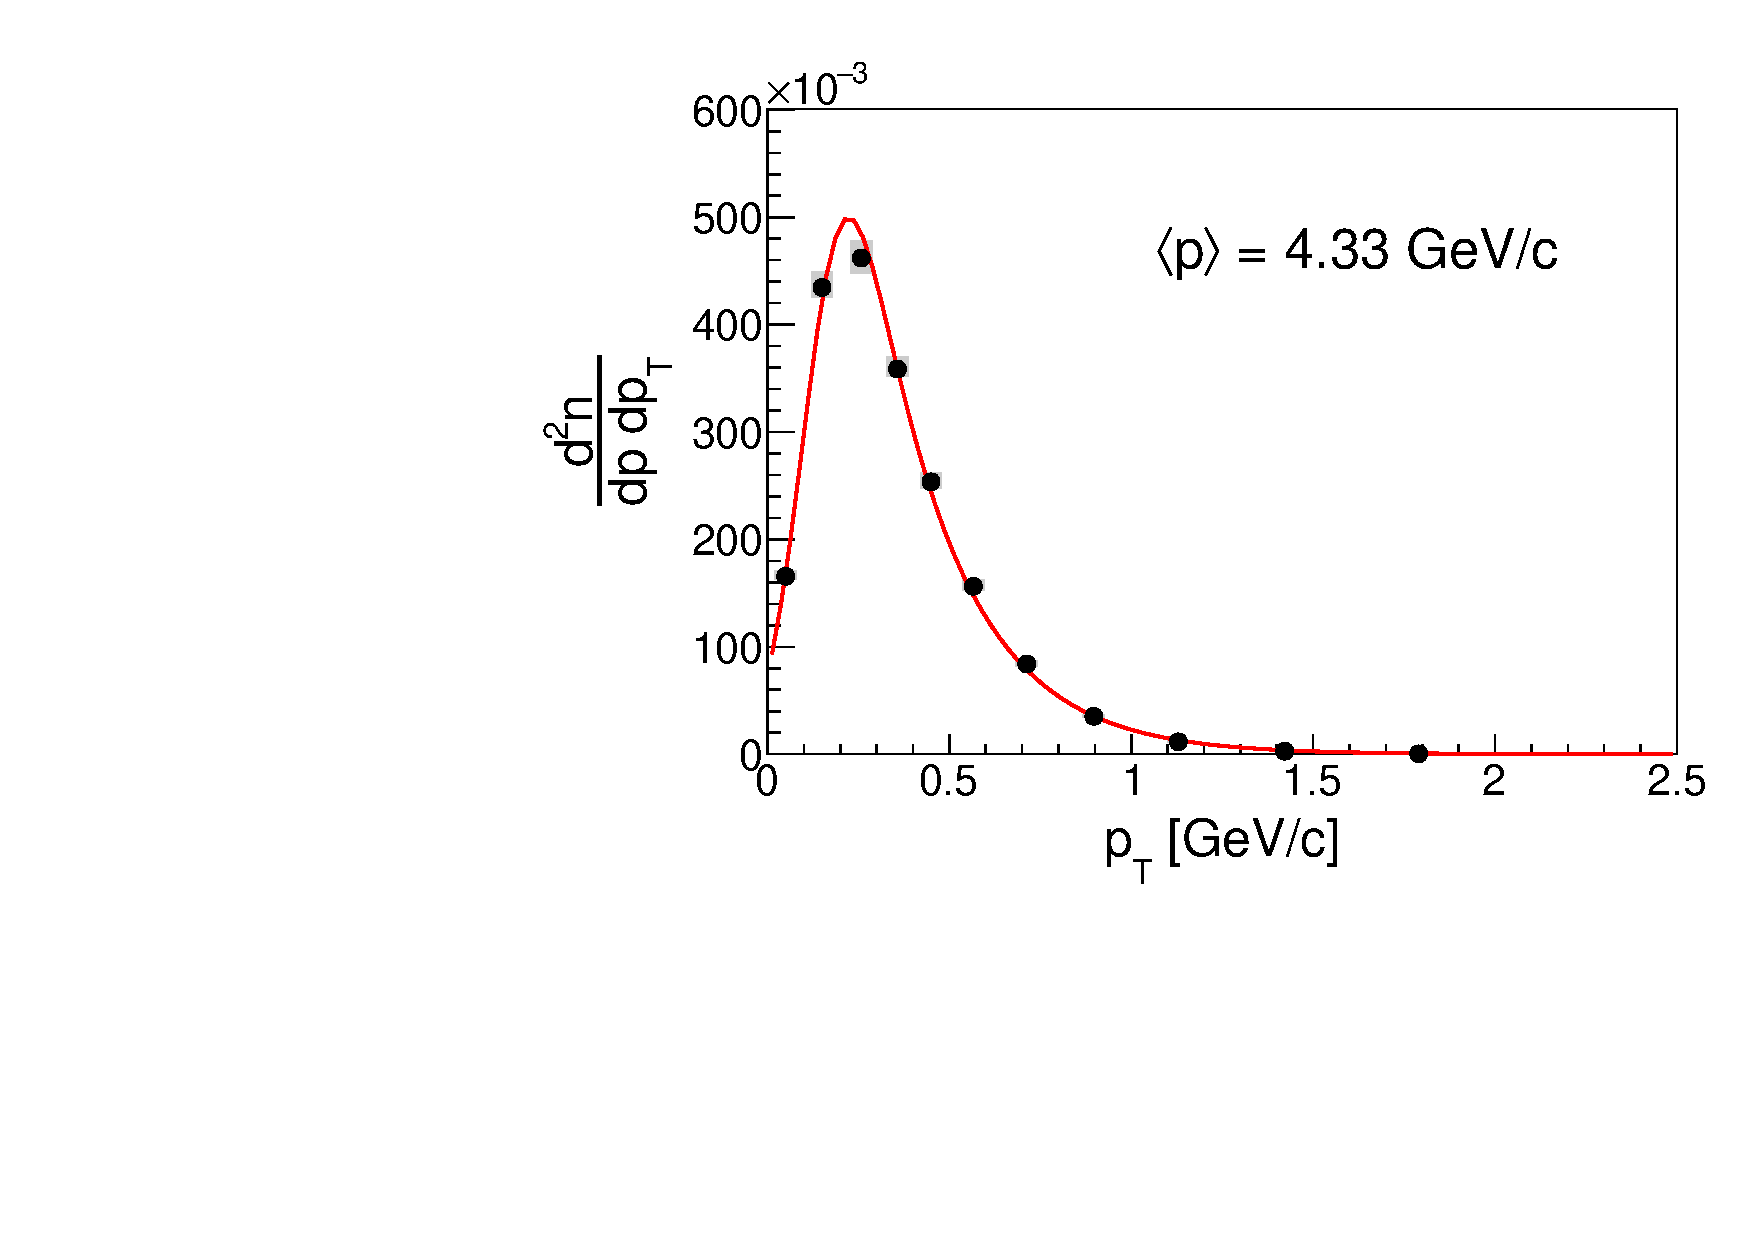
\includegraphics[clip, rviewport=0 0 1 1,width=0.24\textwidth]{spec/spec_pt_158_c1_p1_x17}
  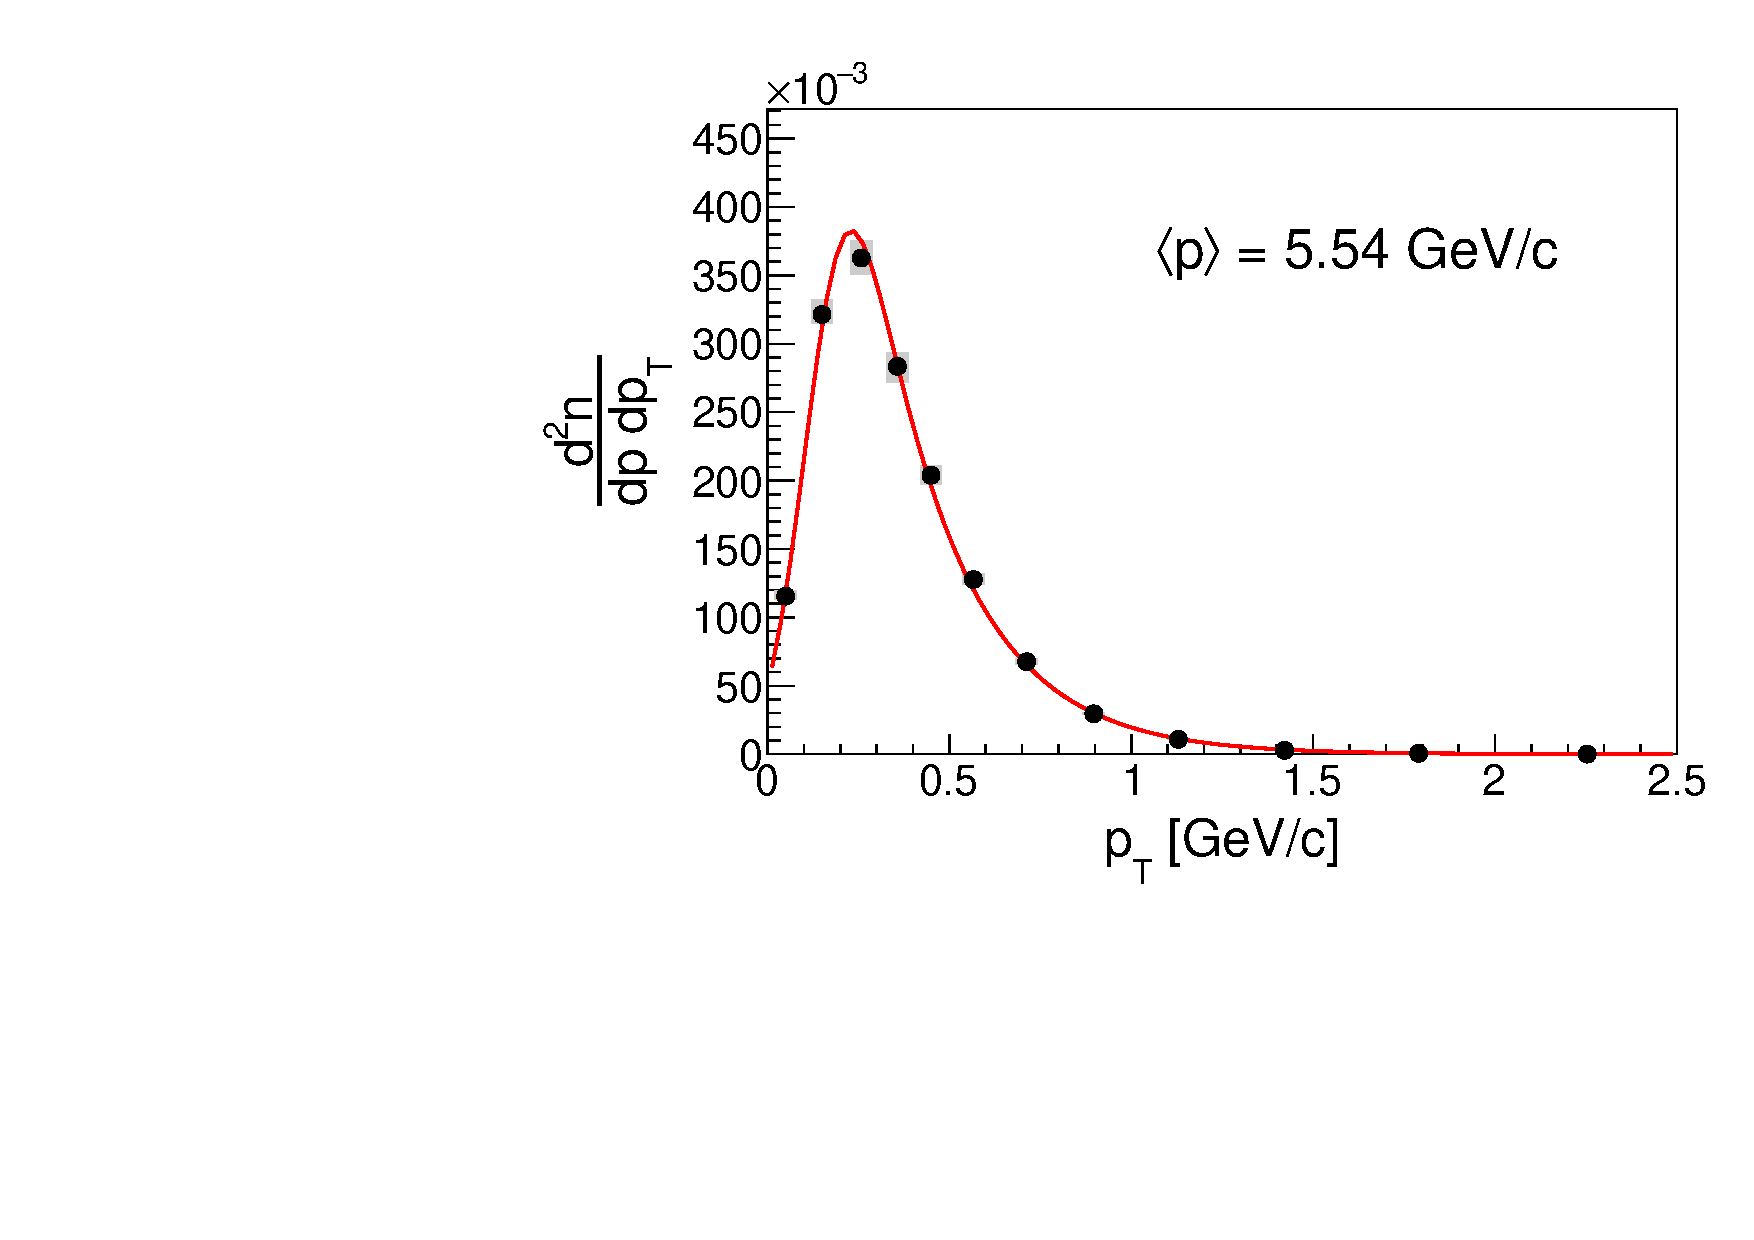
\includegraphics[clip, rviewport=0 0 1 1,width=0.24\textwidth]{spec/spec_pt_158_c1_p1_x18}
  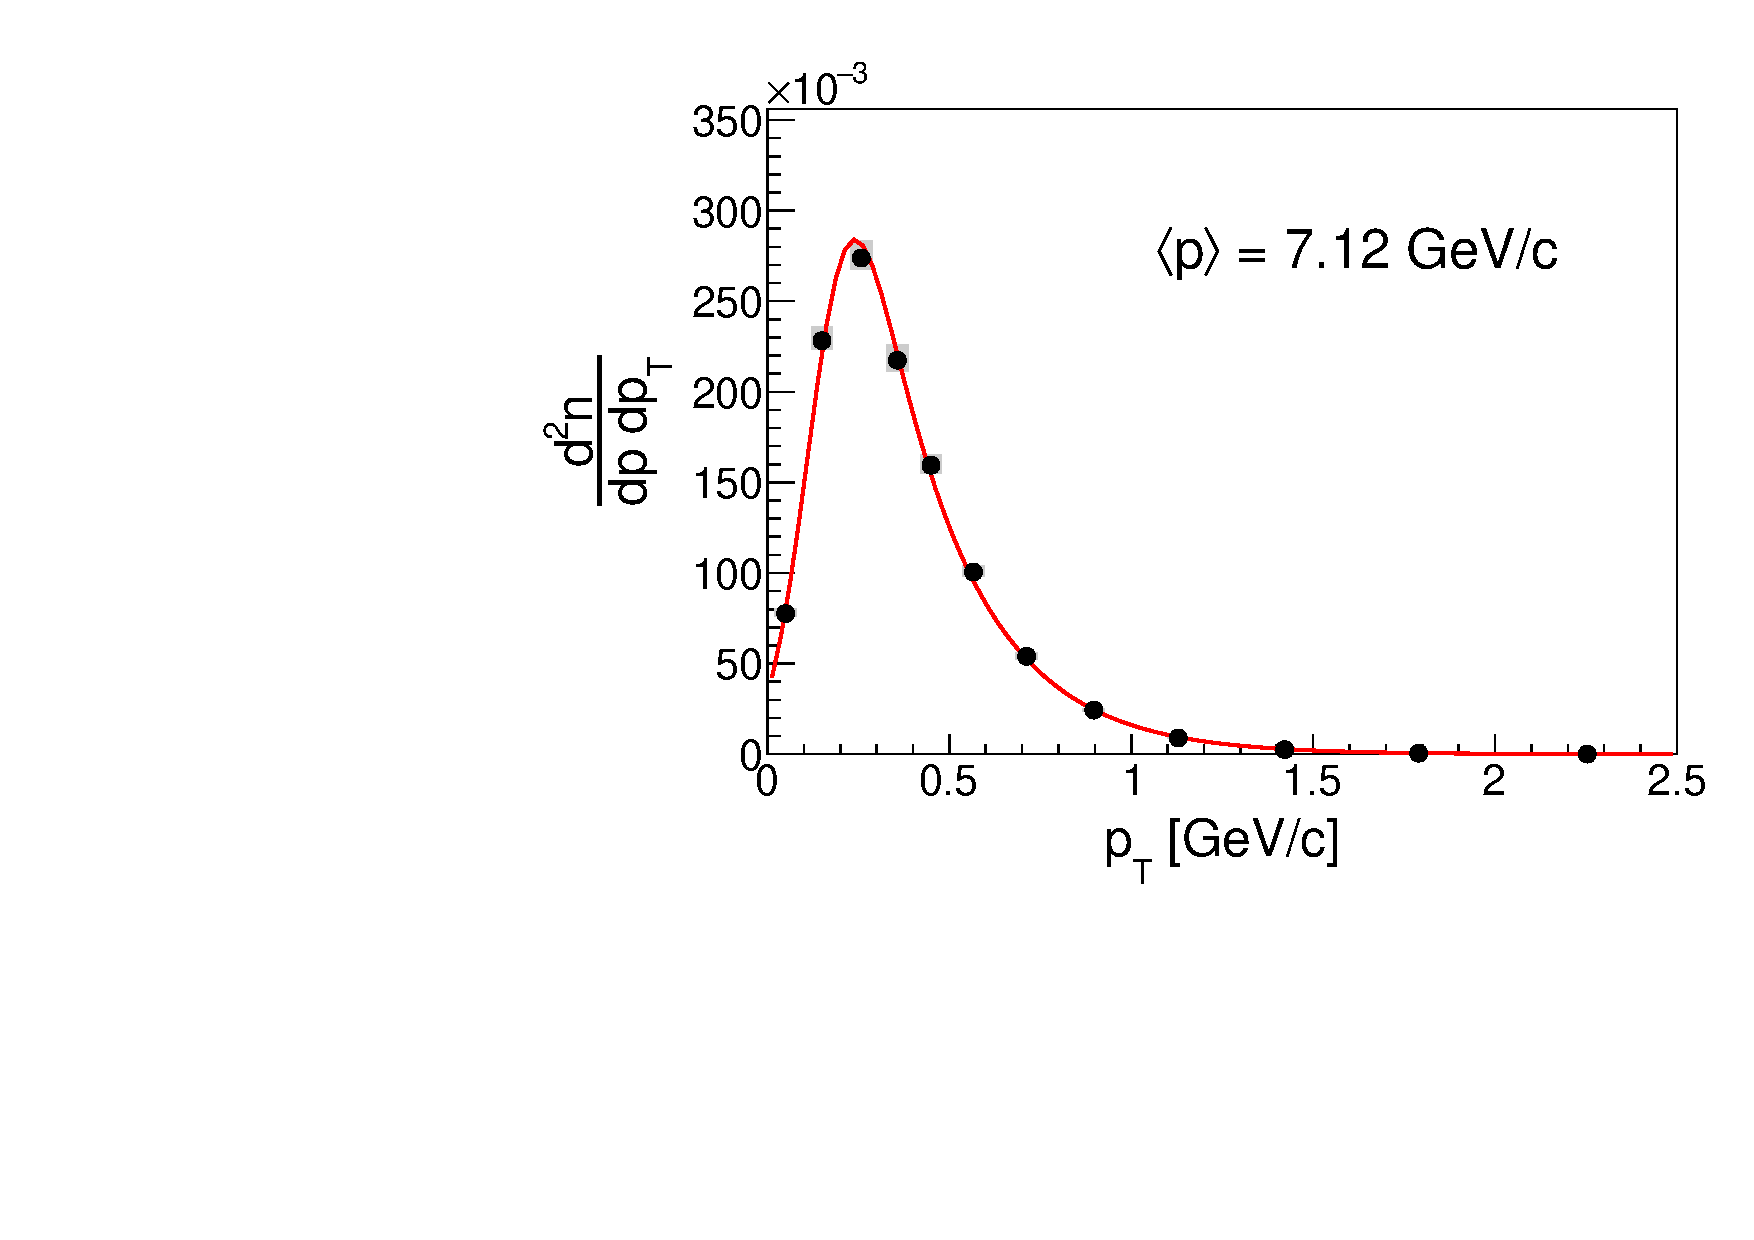
\includegraphics[clip, rviewport=0 0 1 1,width=0.24\textwidth]{spec/spec_pt_158_c1_p1_x19}
  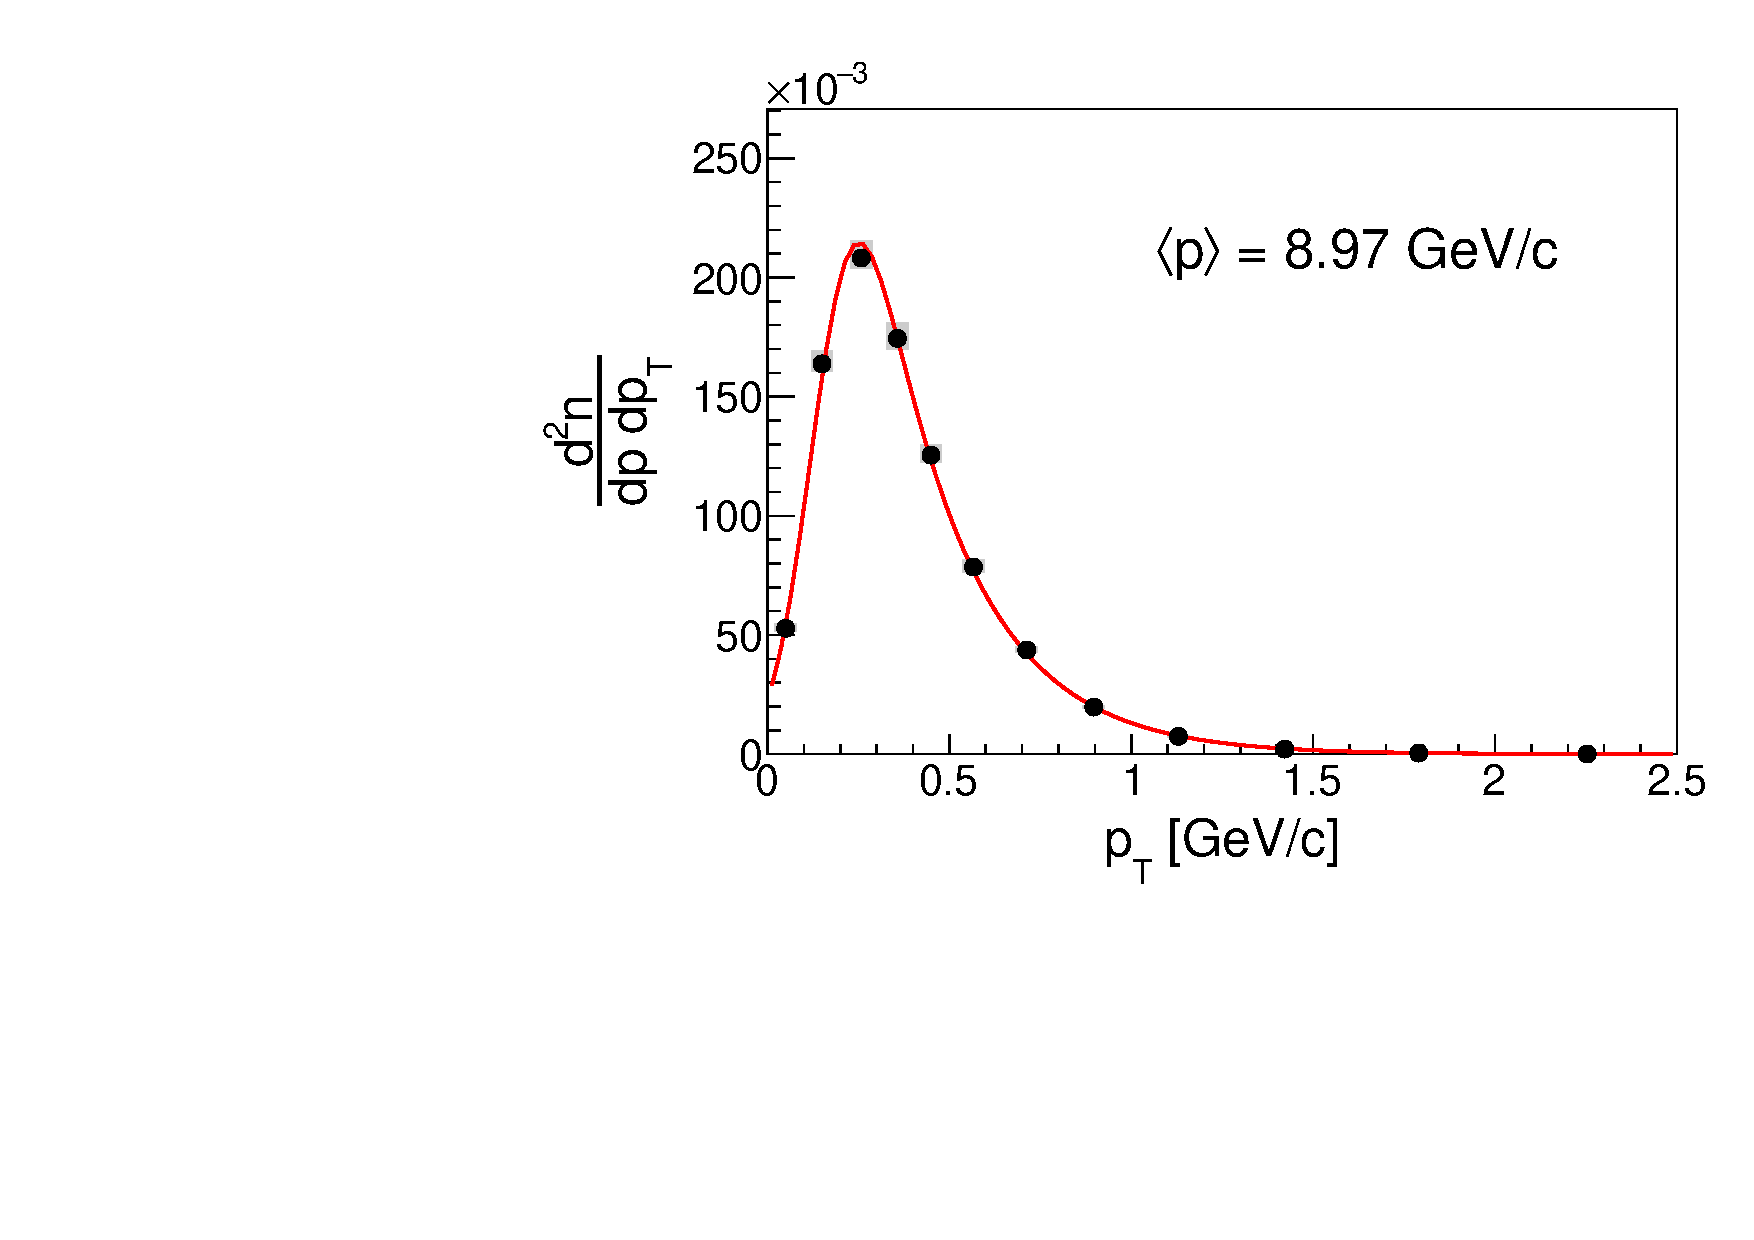
\includegraphics[clip, rviewport=0 0 1 1,width=0.24\textwidth]{spec/spec_pt_158_c1_p1_x20}

  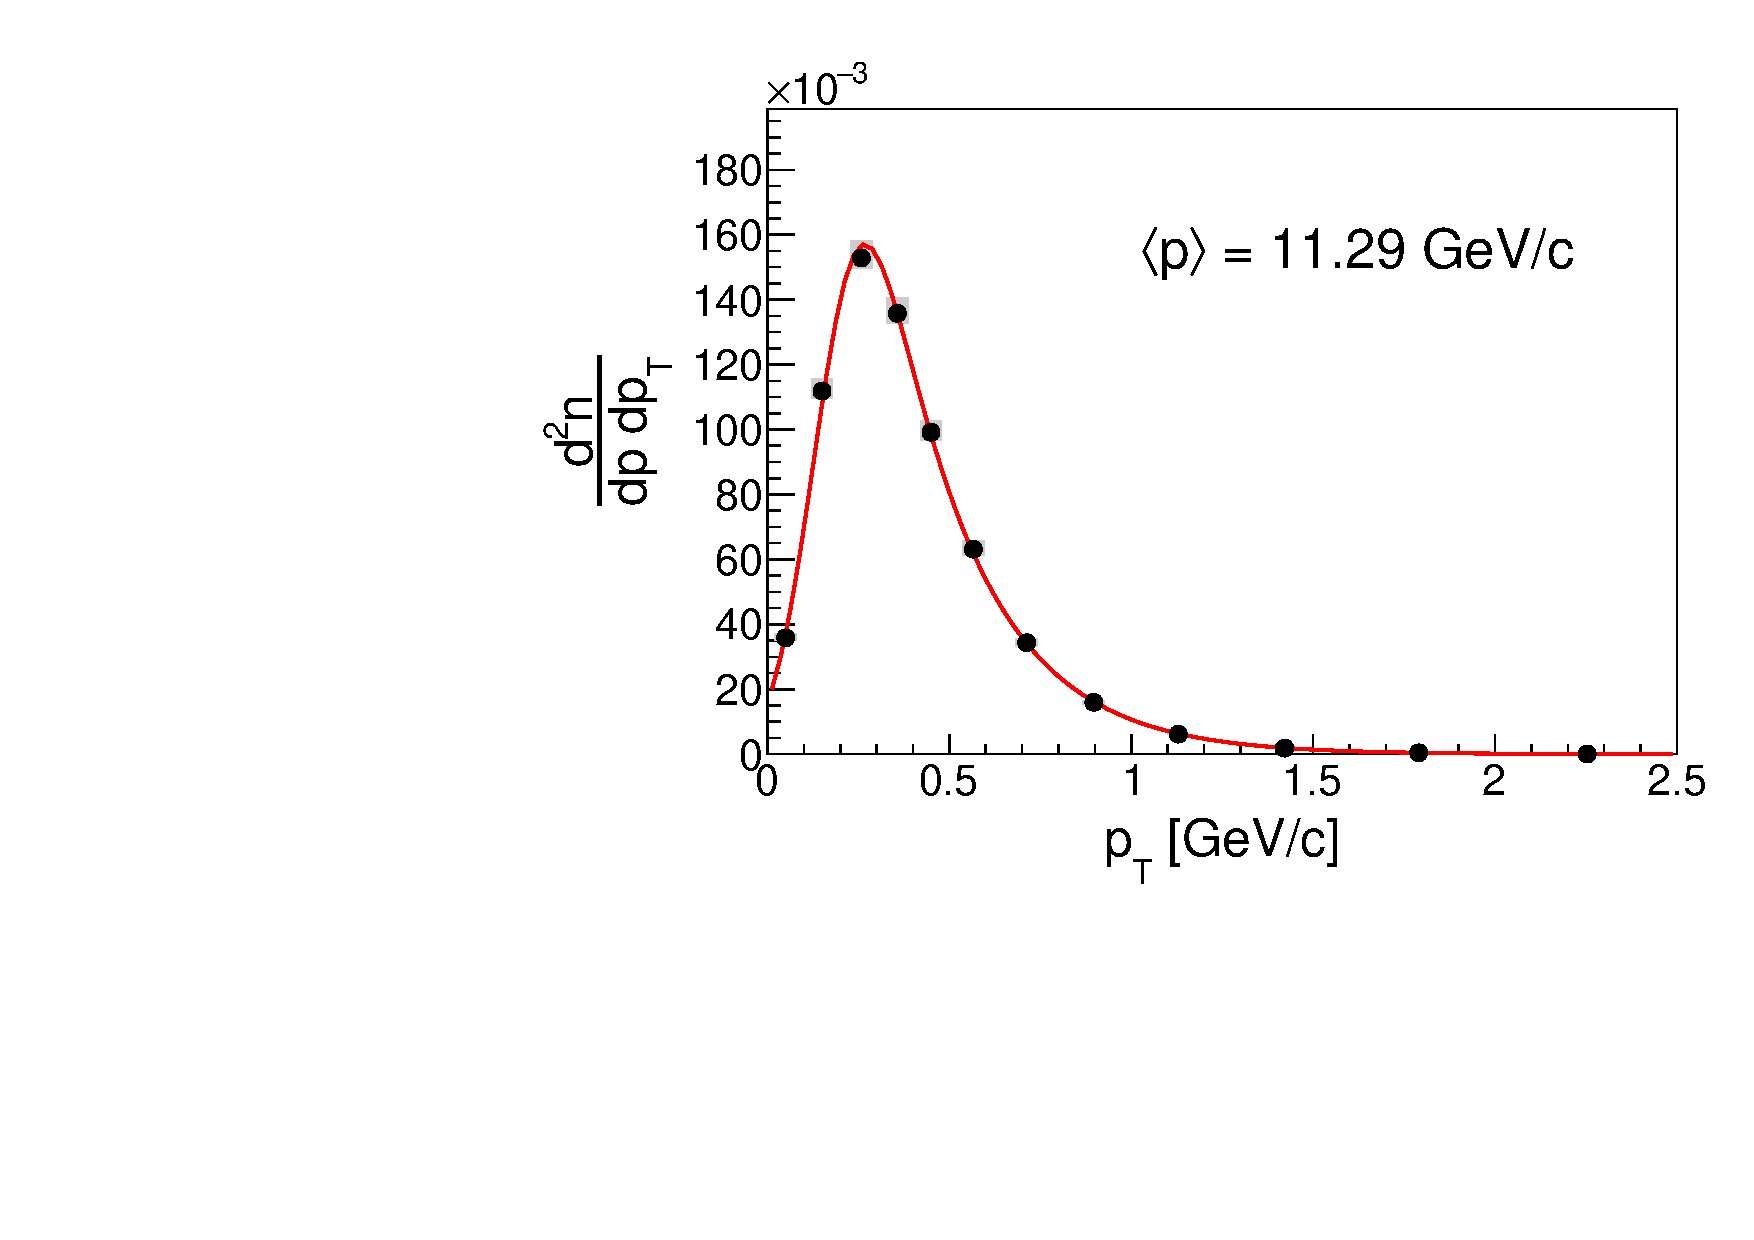
\includegraphics[clip, rviewport=0 0 1 1,width=0.24\textwidth]{spec/spec_pt_158_c1_p1_x21}
  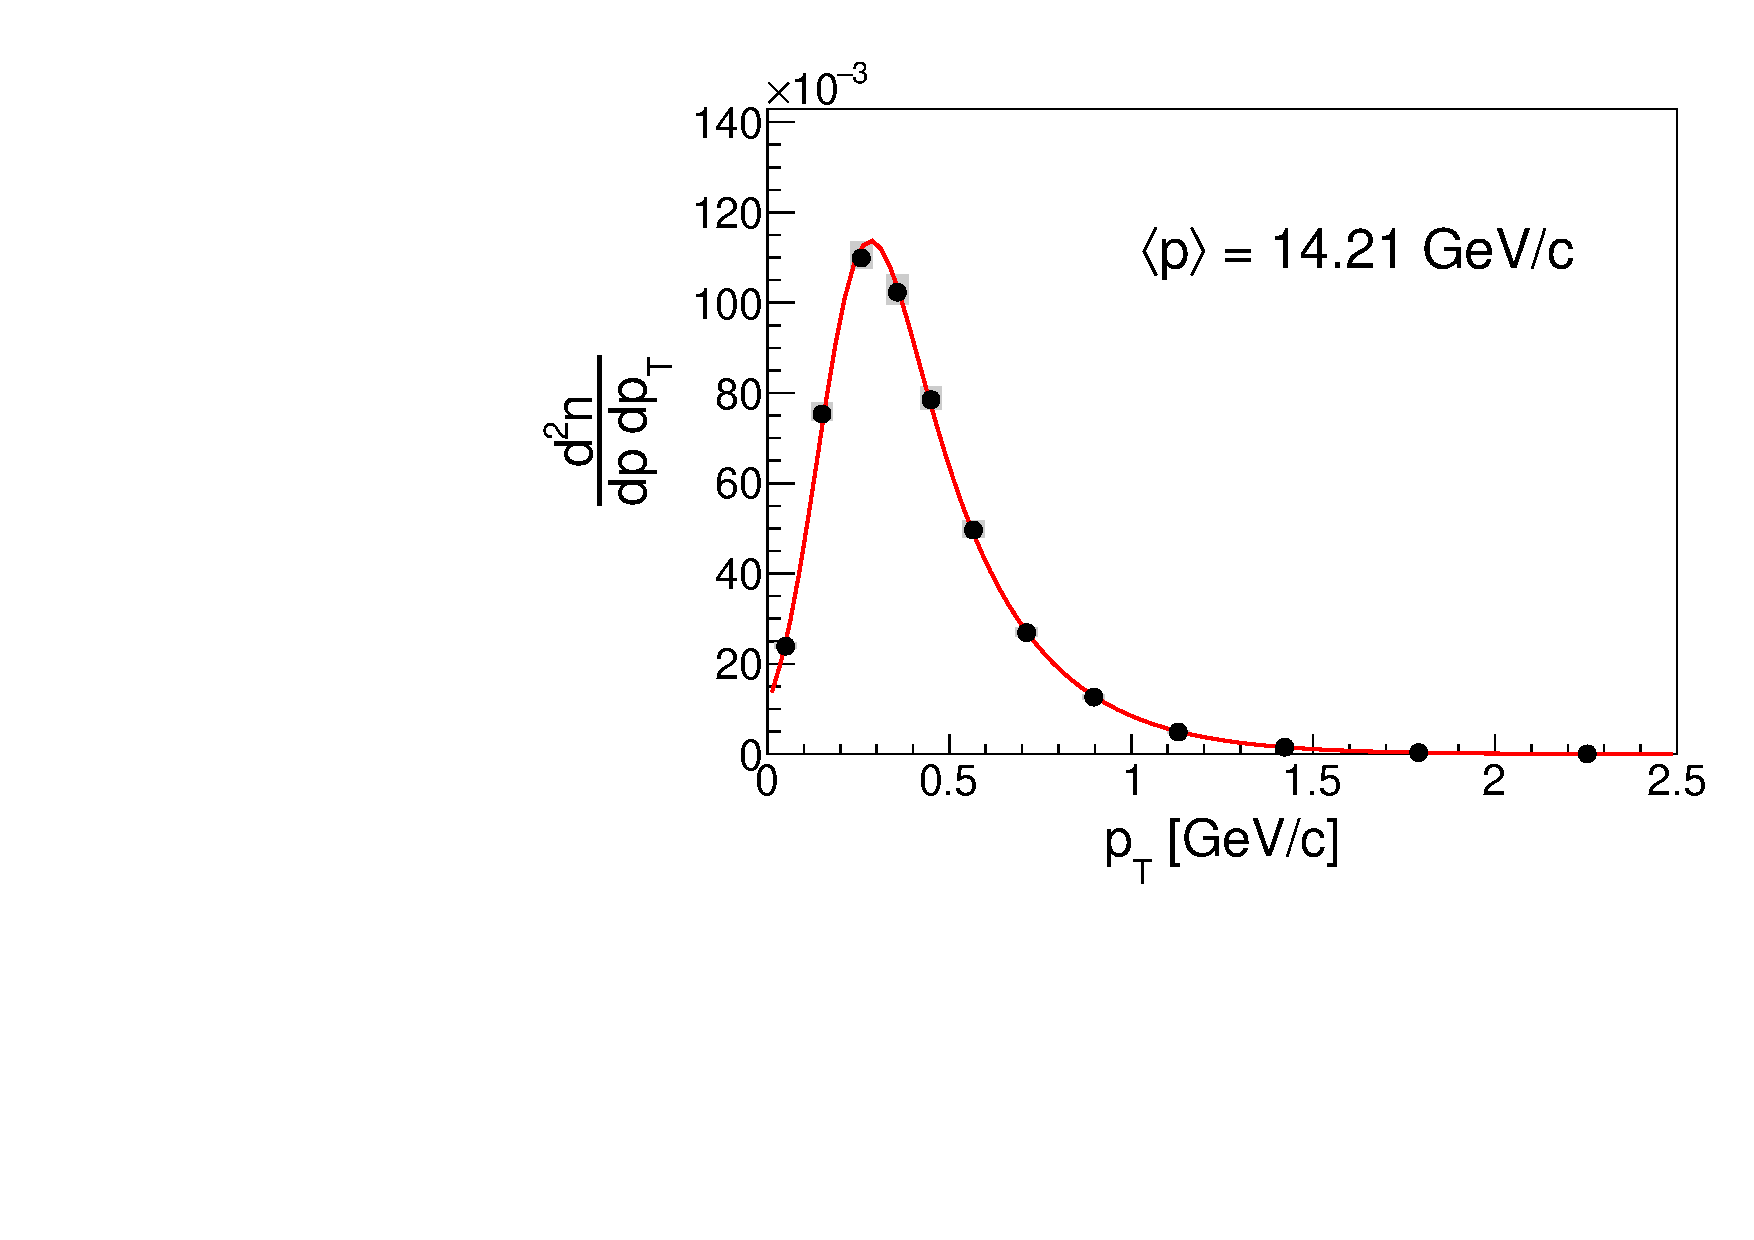
\includegraphics[clip, rviewport=0 0 1 1,width=0.24\textwidth]{spec/spec_pt_158_c1_p1_x22}
  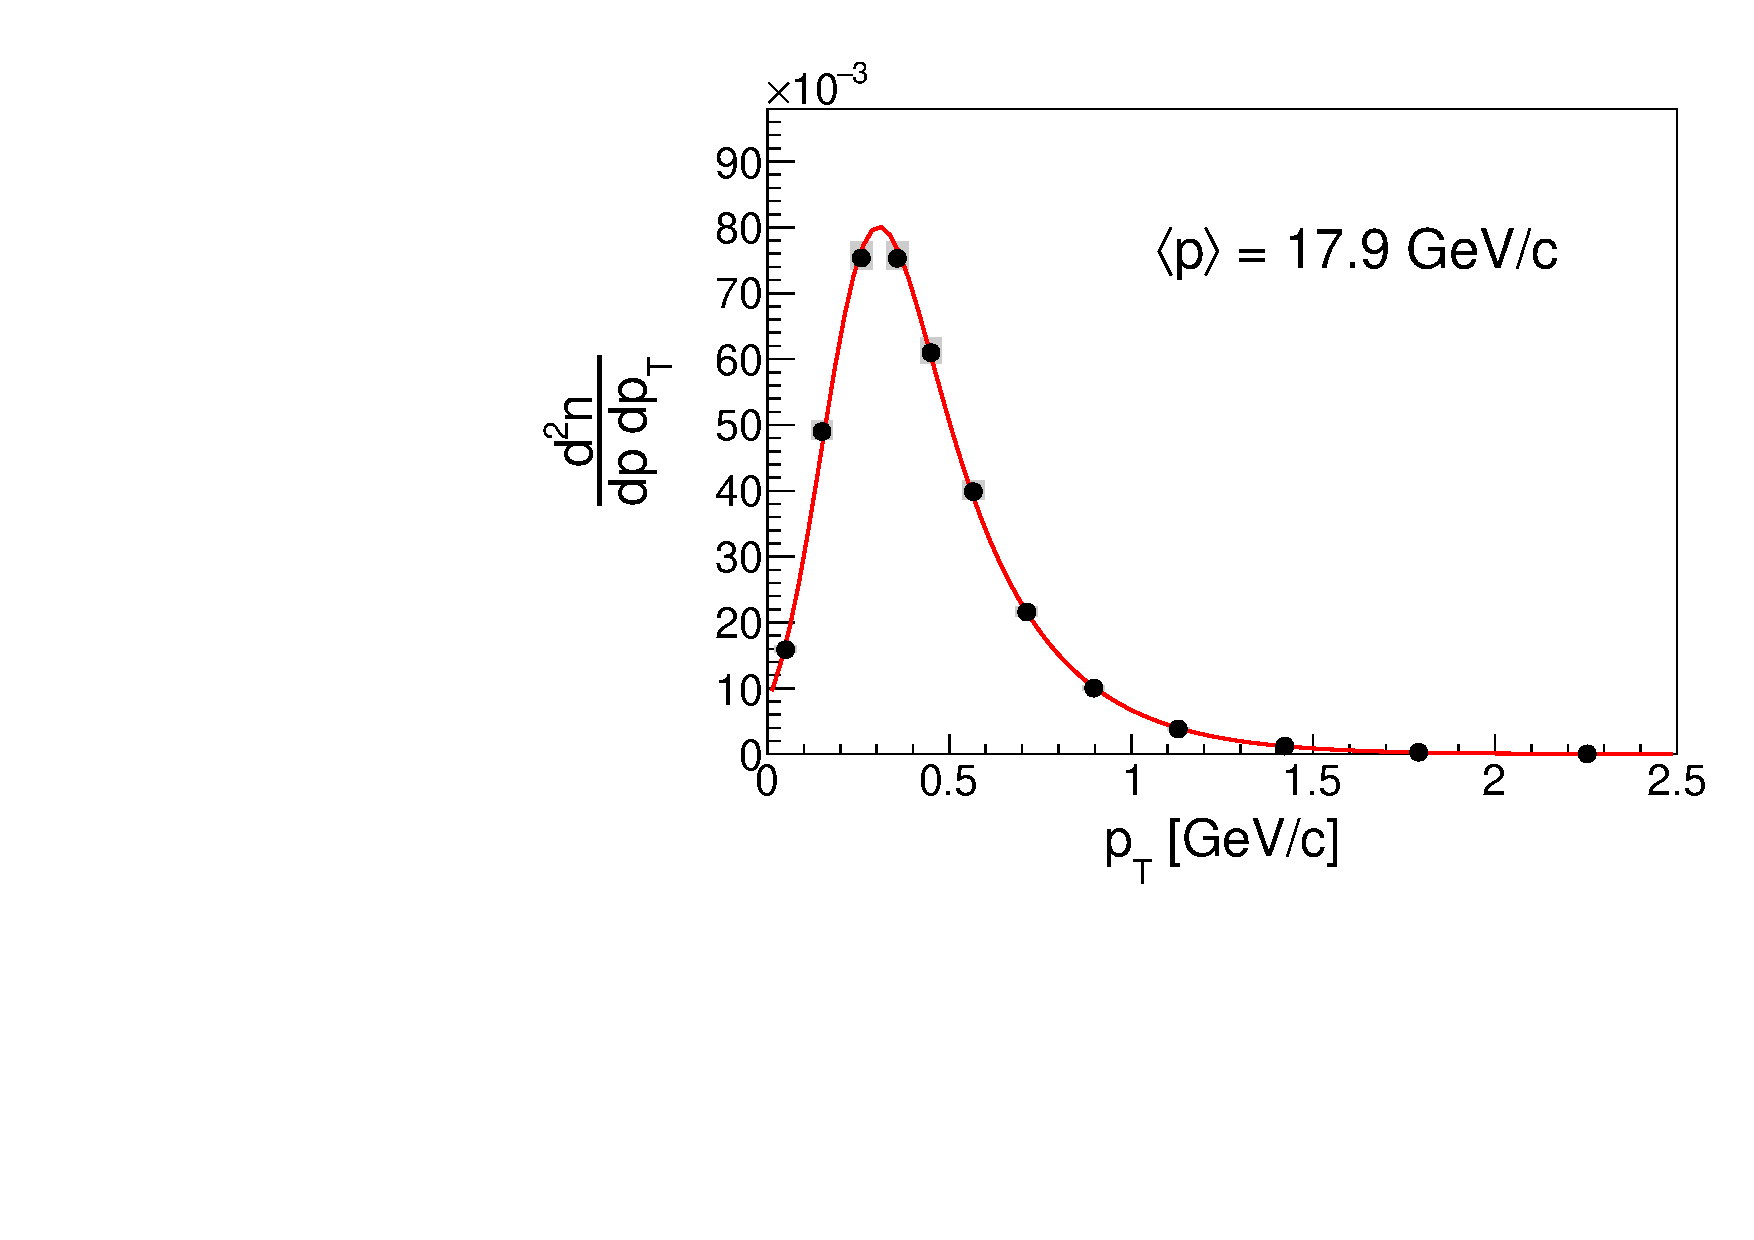
\includegraphics[clip, rviewport=0 0 1 1,width=0.24\textwidth]{spec/spec_pt_158_c1_p1_x23}
  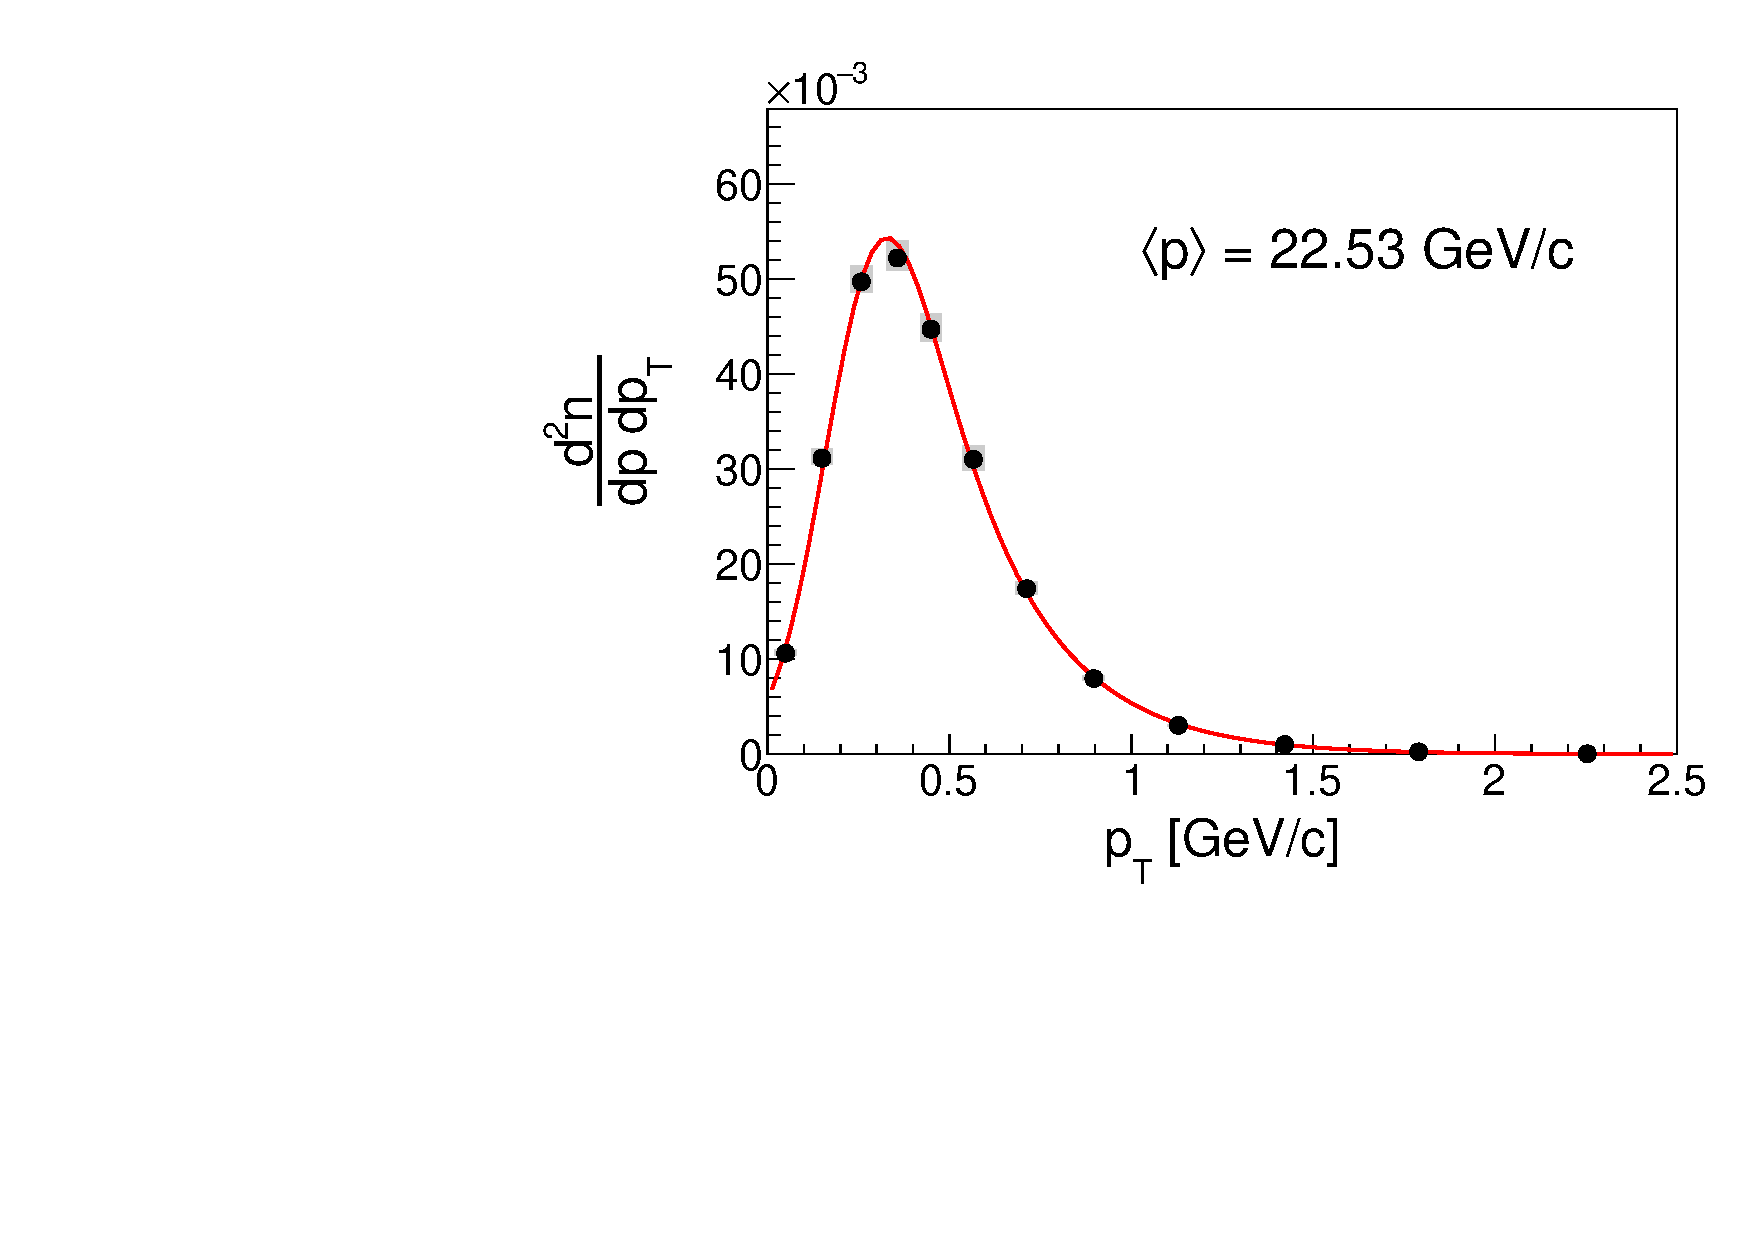
\includegraphics[clip, rviewport=0 0 1 1,width=0.24\textwidth]{spec/spec_pt_158_c1_p1_x24}

  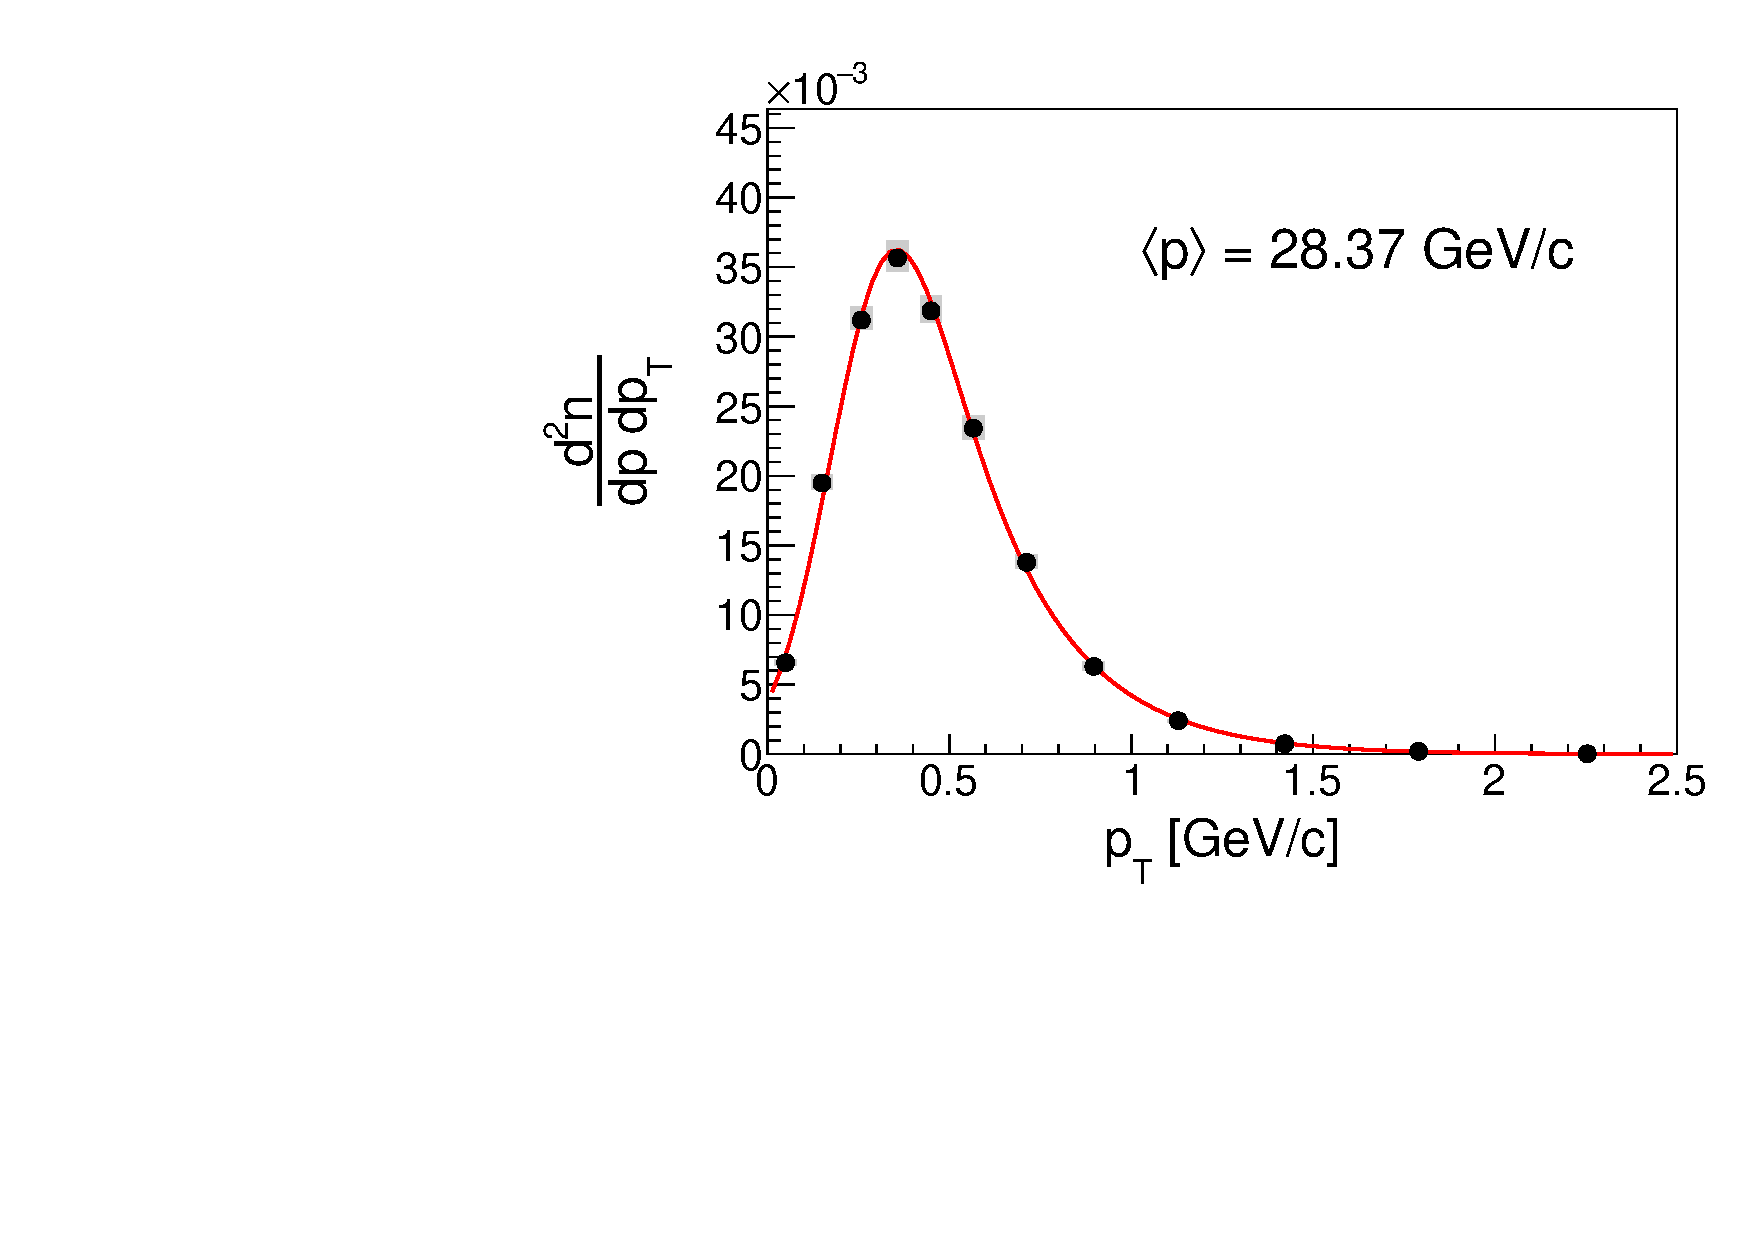
\includegraphics[clip, rviewport=0 0 1 1,width=0.24\textwidth]{spec/spec_pt_158_c1_p1_x25}
  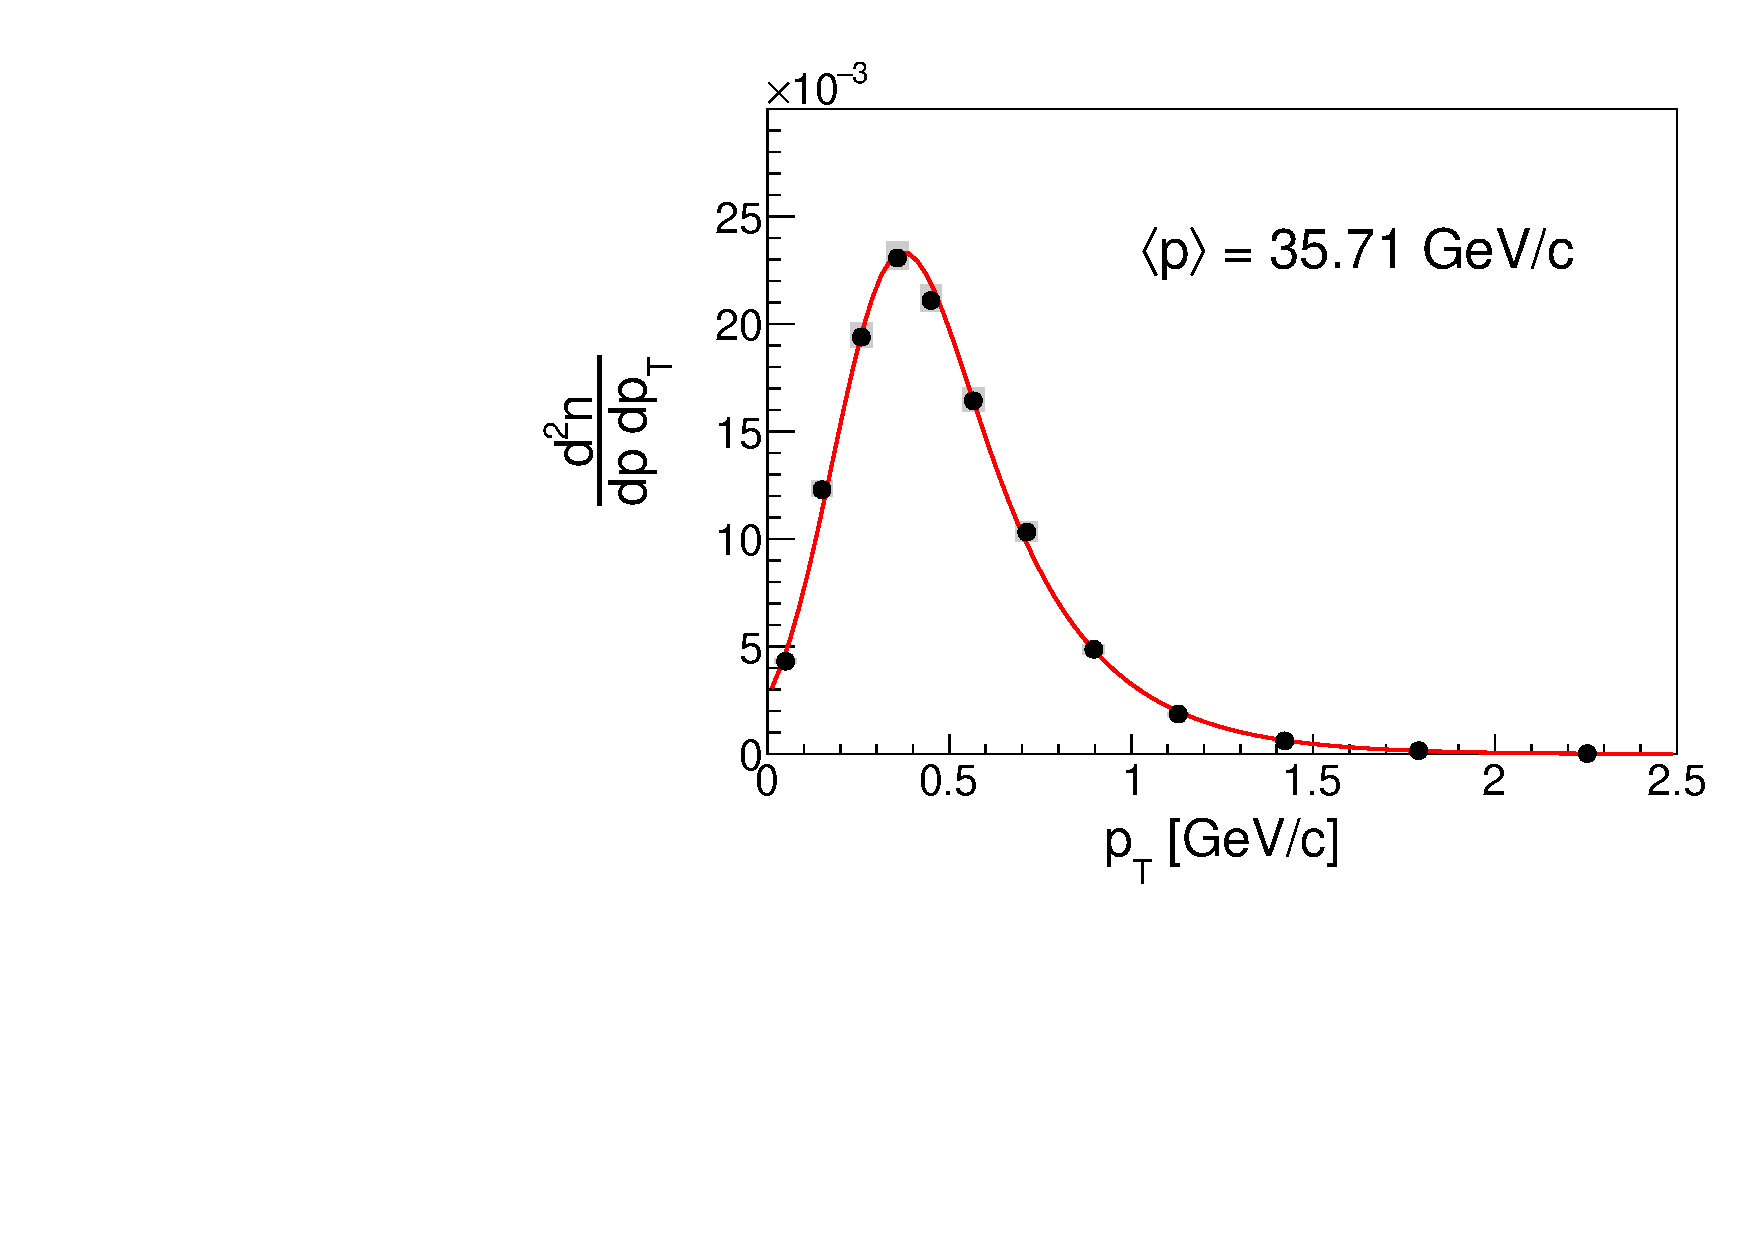
\includegraphics[clip, rviewport=0 0 1 1,width=0.24\textwidth]{spec/spec_pt_158_c1_p1_x26}
  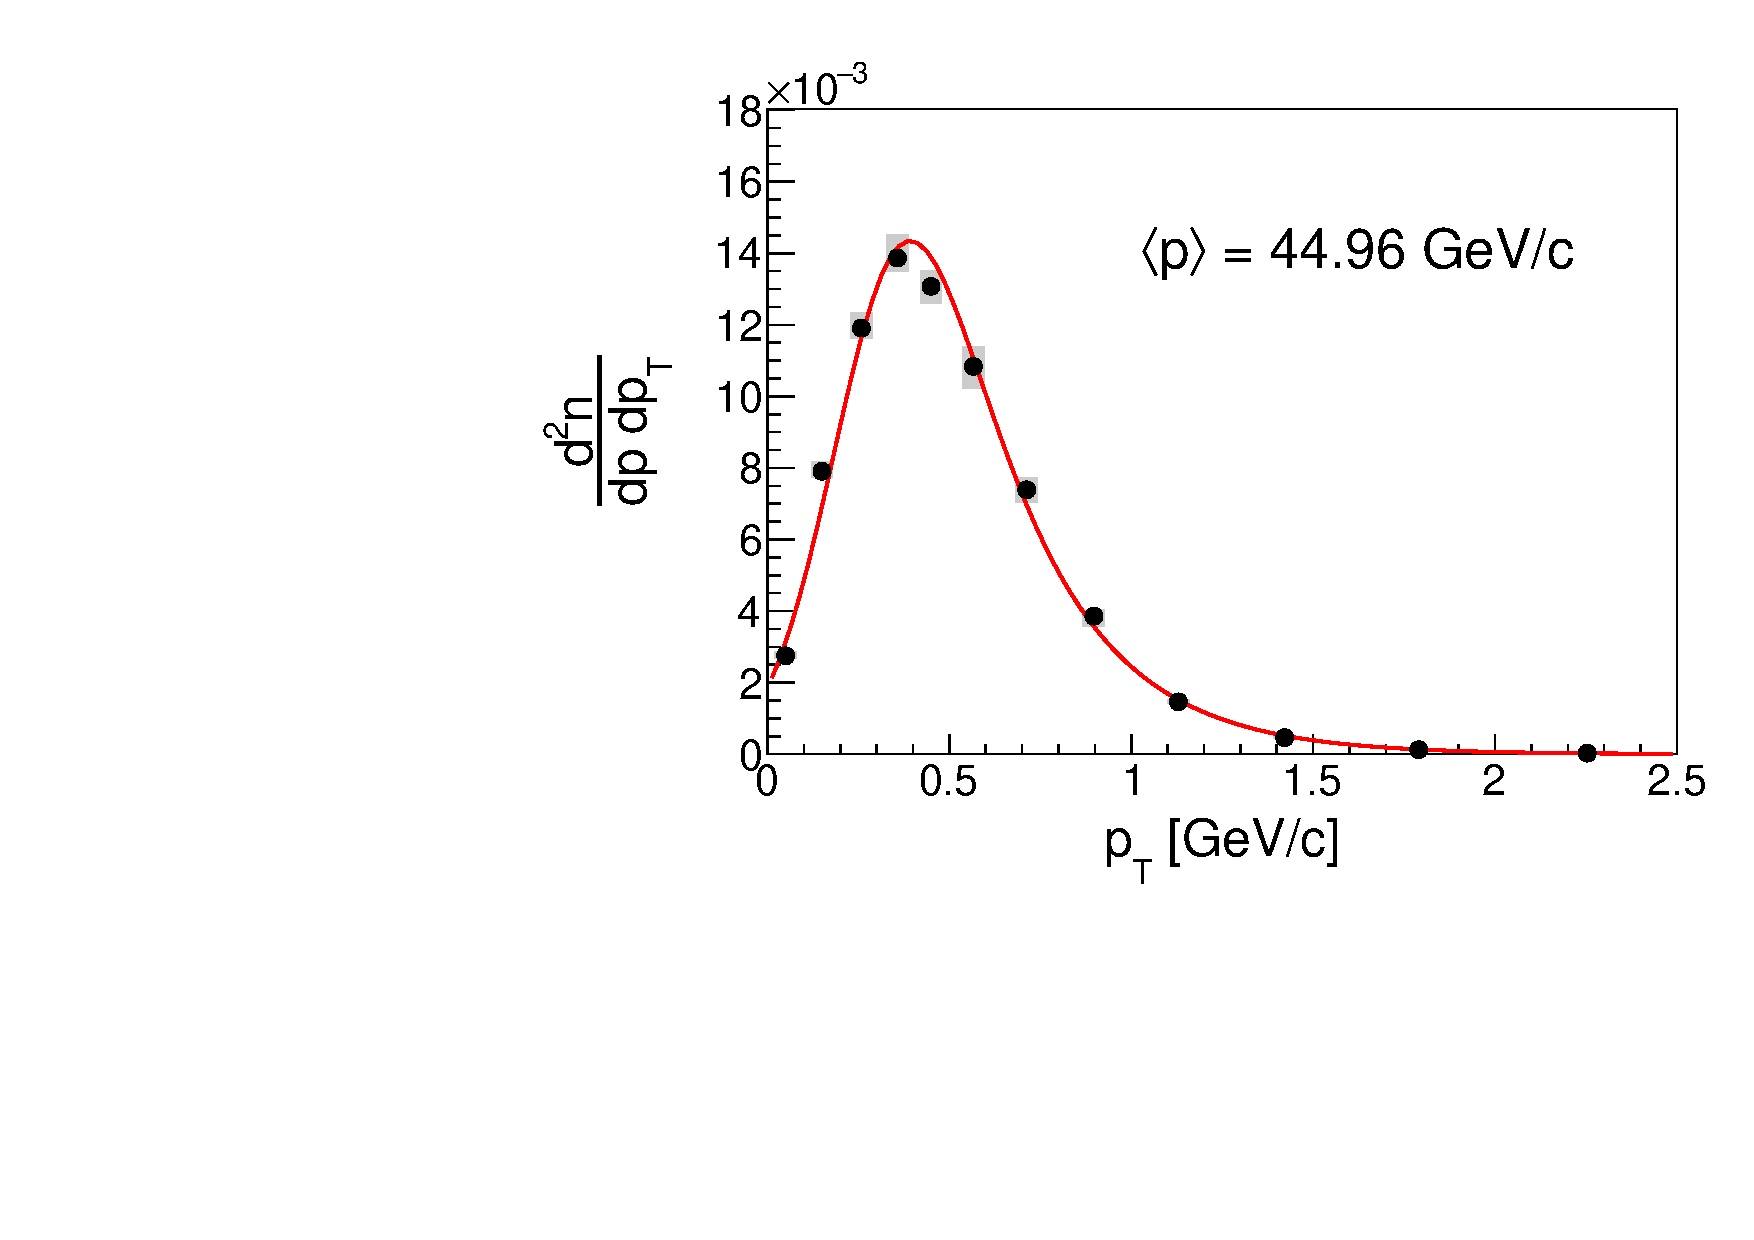
\includegraphics[clip, rviewport=0 0 1 1,width=0.24\textwidth]{spec/spec_pt_158_c1_p1_x27}
  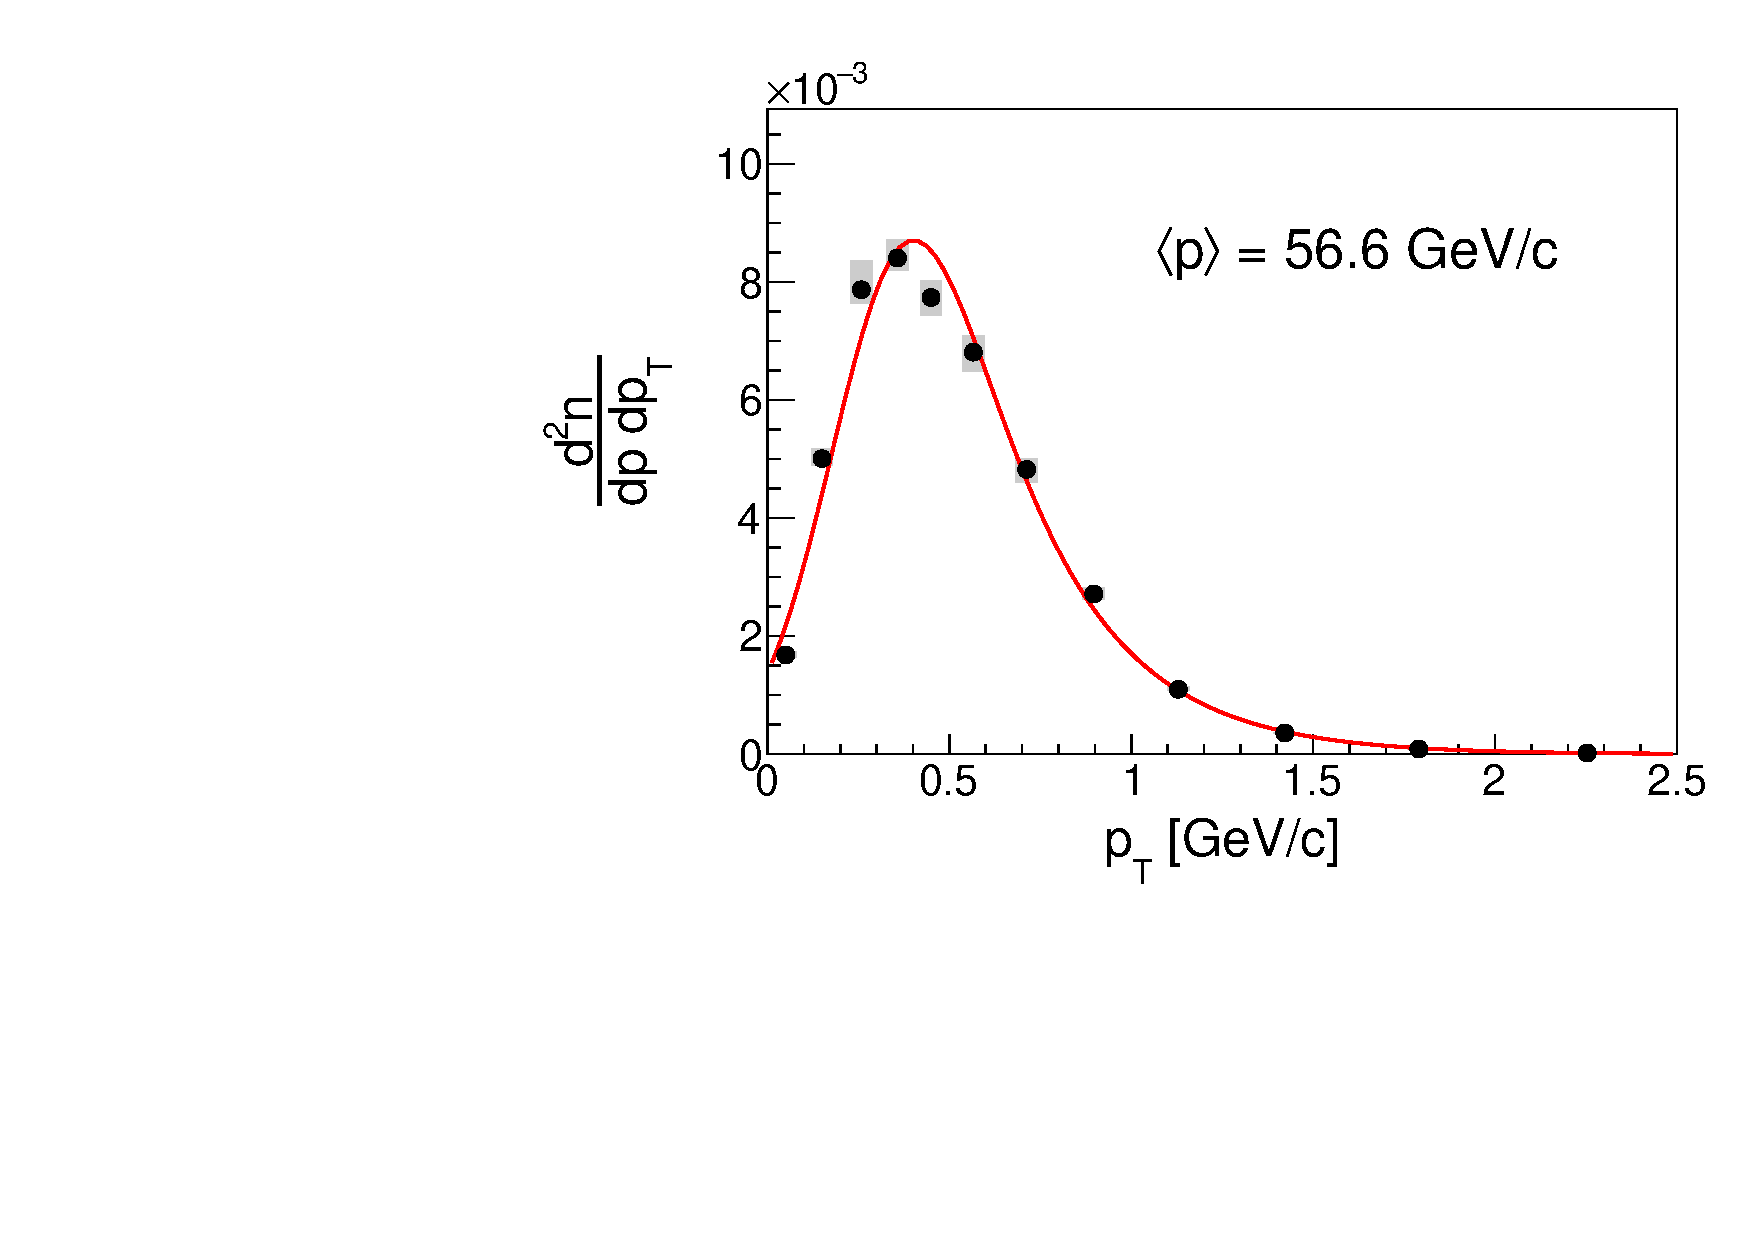
\includegraphics[clip, rviewport=0 0 1 1,width=0.24\textwidth]{spec/spec_pt_158_c1_p1_x28}

  \includegraphics[clip, rviewport=0 0 1 1,width=0.24\textwidth]{spec/spec_pt_158_c1_p1_x29}
  \includegraphics[clip, rviewport=0 0 1 1,width=0.24\textwidth]{spec/spec_pt_158_c1_p1_x30}
  \includegraphics[clip, rviewport=0 0 1 1,width=0.24\textwidth]{spec/spec_pt_158_c1_p1_x31}

  \caption{Double-differential spectra $\frac{\text{d}^2n}{\text{d}\pp\text{d}\pT}$
    of $\pi^-$ for the 158 \GeVc data set. Each plot shows one \pp bins and the value
    of $\langle\pp\rangle$ is indicated inside it. The black lines show the statistical
    uncertainties, while the gray bands show the systematic ones.}
  \label{fig:hadron:spec:dedx:all158:c1p1}
  \begin{center}
    Source: By the author. 
  \end{center}
\end{figure}

%%%%%%%%%% SPEC PT ALL DEDX %%%%%%%%%%%%%%
\begin{figure}[!ht]
  \centering

  \includegraphics[clip, rviewport=0 0 1 1,width=0.24\textwidth]{spec/spec_pt_158_c0_p2_x7}
  \includegraphics[clip, rviewport=0 0 1 1,width=0.24\textwidth]{spec/spec_pt_158_c0_p2_x8}
  \includegraphics[clip, rviewport=0 0 1 1,width=0.24\textwidth]{spec/spec_pt_158_c0_p2_x9}
  \includegraphics[clip, rviewport=0 0 1 1,width=0.24\textwidth]{spec/spec_pt_158_c0_p2_x12}

  \includegraphics[clip, rviewport=0 0 1 1,width=0.24\textwidth]{spec/spec_pt_158_c0_p2_x13}
  \includegraphics[clip, rviewport=0 0 1 1,width=0.24\textwidth]{spec/spec_pt_158_c0_p2_x17}
  \includegraphics[clip, rviewport=0 0 1 1,width=0.24\textwidth]{spec/spec_pt_158_c0_p2_x18}
  \includegraphics[clip, rviewport=0 0 1 1,width=0.24\textwidth]{spec/spec_pt_158_c0_p2_x19}

  \includegraphics[clip, rviewport=0 0 1 1,width=0.24\textwidth]{spec/spec_pt_158_c0_p2_x20}
  \includegraphics[clip, rviewport=0 0 1 1,width=0.24\textwidth]{spec/spec_pt_158_c0_p2_x21}
  \includegraphics[clip, rviewport=0 0 1 1,width=0.24\textwidth]{spec/spec_pt_158_c0_p2_x22}
  \includegraphics[clip, rviewport=0 0 1 1,width=0.24\textwidth]{spec/spec_pt_158_c0_p2_x23}

  \includegraphics[clip, rviewport=0 0 1 1,width=0.24\textwidth]{spec/spec_pt_158_c0_p2_x24}
  \includegraphics[clip, rviewport=0 0 1 1,width=0.24\textwidth]{spec/spec_pt_158_c0_p2_x25}
  \includegraphics[clip, rviewport=0 0 1 1,width=0.24\textwidth]{spec/spec_pt_158_c0_p2_x26}
  \includegraphics[clip, rviewport=0 0 1 1,width=0.24\textwidth]{spec/spec_pt_158_c0_p2_x27}

  \includegraphics[clip, rviewport=0 0 1 1,width=0.24\textwidth]{spec/spec_pt_158_c0_p2_x28}
  \includegraphics[clip, rviewport=0 0 1 1,width=0.24\textwidth]{spec/spec_pt_158_c0_p2_x29}

  \caption{Double-differential spectra $\frac{\text{d}^2n}{\text{d}\pp\text{d}\pT}$
    of K$^+$ for the 158 \GeVc data set. Each plot shows one \pp bins and the value
    of $\langle\pp\rangle$ is indicated inside it. The black lines show the statistical
    uncertainties, while the gray bands show the systematic ones.}
  \label{fig:hadron:spec:dedx:all158:c0p2}
  \begin{center}
    Source: By the author. 
  \end{center}
\end{figure}

%%%%%%%%%% SPEC PT ALL DEDX %%%%%%%%%%%%%%
\begin{figure}[!ht]
  \centering

  \includegraphics[clip, rviewport=0 0 1 1,width=0.24\textwidth]{spec/spec_pt_158_c1_p2_x8}
  \includegraphics[clip, rviewport=0 0 1 1,width=0.24\textwidth]{spec/spec_pt_158_c1_p2_x12}
  \includegraphics[clip, rviewport=0 0 1 1,width=0.24\textwidth]{spec/spec_pt_158_c1_p2_x13}
  \includegraphics[clip, rviewport=0 0 1 1,width=0.24\textwidth]{spec/spec_pt_158_c1_p2_x16}
  
  \includegraphics[clip, rviewport=0 0 1 1,width=0.24\textwidth]{spec/spec_pt_158_c1_p2_x17}
  \includegraphics[clip, rviewport=0 0 1 1,width=0.24\textwidth]{spec/spec_pt_158_c1_p2_x18}
  \includegraphics[clip, rviewport=0 0 1 1,width=0.24\textwidth]{spec/spec_pt_158_c1_p2_x19}
  \includegraphics[clip, rviewport=0 0 1 1,width=0.24\textwidth]{spec/spec_pt_158_c1_p2_x20}

  \includegraphics[clip, rviewport=0 0 1 1,width=0.24\textwidth]{spec/spec_pt_158_c1_p2_x21}
  \includegraphics[clip, rviewport=0 0 1 1,width=0.24\textwidth]{spec/spec_pt_158_c1_p2_x22}
  \includegraphics[clip, rviewport=0 0 1 1,width=0.24\textwidth]{spec/spec_pt_158_c1_p2_x23}
  \includegraphics[clip, rviewport=0 0 1 1,width=0.24\textwidth]{spec/spec_pt_158_c1_p2_x24}

  \includegraphics[clip, rviewport=0 0 1 1,width=0.24\textwidth]{spec/spec_pt_158_c1_p2_x25}
  \includegraphics[clip, rviewport=0 0 1 1,width=0.24\textwidth]{spec/spec_pt_158_c1_p2_x26}
  \includegraphics[clip, rviewport=0 0 1 1,width=0.24\textwidth]{spec/spec_pt_158_c1_p2_x27}
  \includegraphics[clip, rviewport=0 0 1 1,width=0.24\textwidth]{spec/spec_pt_158_c1_p2_x28}

  \includegraphics[clip, rviewport=0 0 1 1,width=0.24\textwidth]{spec/spec_pt_158_c1_p2_x29}

  \caption{Double-differential spectra $\frac{\text{d}^2n}{\text{d}\pp\text{d}\pT}$
    of K$^-$ for the 158 \GeVc data set. Each plot shows one \pp bins and the value
    of $\langle\pp\rangle$ is indicated inside it. The black lines show the statistical
    uncertainties, while the gray bands show the systematic ones.}
  \label{fig:hadron:spec:dedx:all158:c1p2}
  \begin{center}
    Source: By the author. 
  \end{center}
\end{figure}

%%%%%%%%%% SPEC PT ALL DEDX %%%%%%%%%%%%%%
\begin{figure}[!ht]
  \centering

  \includegraphics[clip, rviewport=0 0 1 1,width=0.24\textwidth]{spec/spec_pt_158_c0_p3_x7}
  \includegraphics[clip, rviewport=0 0 1 1,width=0.24\textwidth]{spec/spec_pt_158_c0_p3_x8}
  \includegraphics[clip, rviewport=0 0 1 1,width=0.24\textwidth]{spec/spec_pt_158_c0_p3_x9}
  \includegraphics[clip, rviewport=0 0 1 1,width=0.24\textwidth]{spec/spec_pt_158_c0_p3_x10}

  \includegraphics[clip, rviewport=0 0 1 1,width=0.24\textwidth]{spec/spec_pt_158_c0_p3_x11}
  \includegraphics[clip, rviewport=0 0 1 1,width=0.24\textwidth]{spec/spec_pt_158_c0_p3_x13}
  \includegraphics[clip, rviewport=0 0 1 1,width=0.24\textwidth]{spec/spec_pt_158_c0_p3_x15}
  \includegraphics[clip, rviewport=0 0 1 1,width=0.24\textwidth]{spec/spec_pt_158_c0_p3_x16}

  \includegraphics[clip, rviewport=0 0 1 1,width=0.24\textwidth]{spec/spec_pt_158_c0_p3_x17}
  \includegraphics[clip, rviewport=0 0 1 1,width=0.24\textwidth]{spec/spec_pt_158_c0_p3_x18}
  \includegraphics[clip, rviewport=0 0 1 1,width=0.24\textwidth]{spec/spec_pt_158_c0_p3_x19}
  \includegraphics[clip, rviewport=0 0 1 1,width=0.24\textwidth]{spec/spec_pt_158_c0_p3_x20}

  \includegraphics[clip, rviewport=0 0 1 1,width=0.24\textwidth]{spec/spec_pt_158_c0_p3_x21}
  \includegraphics[clip, rviewport=0 0 1 1,width=0.24\textwidth]{spec/spec_pt_158_c0_p3_x22}
  \includegraphics[clip, rviewport=0 0 1 1,width=0.24\textwidth]{spec/spec_pt_158_c0_p3_x23}
  \includegraphics[clip, rviewport=0 0 1 1,width=0.24\textwidth]{spec/spec_pt_158_c0_p3_x24}

  \includegraphics[clip, rviewport=0 0 1 1,width=0.24\textwidth]{spec/spec_pt_158_c0_p3_x25}
  \includegraphics[clip, rviewport=0 0 1 1,width=0.24\textwidth]{spec/spec_pt_158_c0_p3_x26}
  \includegraphics[clip, rviewport=0 0 1 1,width=0.24\textwidth]{spec/spec_pt_158_c0_p3_x27}
  \includegraphics[clip, rviewport=0 0 1 1,width=0.24\textwidth]{spec/spec_pt_158_c0_p3_x28}

  \includegraphics[clip, rviewport=0 0 1 1,width=0.24\textwidth]{spec/spec_pt_158_c0_p3_x29}
  \includegraphics[clip, rviewport=0 0 1 1,width=0.24\textwidth]{spec/spec_pt_158_c0_p3_x30}

  \caption{Double-differential spectra $\frac{\text{d}^2n}{\text{d}\pp\text{d}\pT}$
    of p$^+$ for the 158 \GeVc data set. Each plot shows one \pp bins and the value
    of $\langle\pp\rangle$ is indicated inside it. The black lines show the statistical
    uncertainties, while the gray bands show the systematic ones.}
  \label{fig:hadron:spec:dedx:all158:c0p3}
  \begin{center}
    Source: By the author. 
  \end{center}
\end{figure}

%%%%%%%%%% SPEC PT ALL DEDX %%%%%%%%%%%%%%
\begin{figure}[!ht]
  \centering

  \includegraphics[clip, rviewport=0 0 1 1,width=0.24\textwidth]{spec/spec_pt_158_c0_p3_x16}
  \includegraphics[clip, rviewport=0 0 1 1,width=0.24\textwidth]{spec/spec_pt_158_c0_p3_x17}
  \includegraphics[clip, rviewport=0 0 1 1,width=0.24\textwidth]{spec/spec_pt_158_c0_p3_x18}
  \includegraphics[clip, rviewport=0 0 1 1,width=0.24\textwidth]{spec/spec_pt_158_c0_p3_x19}

  \includegraphics[clip, rviewport=0 0 1 1,width=0.24\textwidth]{spec/spec_pt_158_c0_p3_x20}
  \includegraphics[clip, rviewport=0 0 1 1,width=0.24\textwidth]{spec/spec_pt_158_c0_p3_x21}
  \includegraphics[clip, rviewport=0 0 1 1,width=0.24\textwidth]{spec/spec_pt_158_c0_p3_x22}
  \includegraphics[clip, rviewport=0 0 1 1,width=0.24\textwidth]{spec/spec_pt_158_c0_p3_x23}

  \includegraphics[clip, rviewport=0 0 1 1,width=0.24\textwidth]{spec/spec_pt_158_c0_p3_x24}
  \includegraphics[clip, rviewport=0 0 1 1,width=0.24\textwidth]{spec/spec_pt_158_c0_p3_x25}
  \includegraphics[clip, rviewport=0 0 1 1,width=0.24\textwidth]{spec/spec_pt_158_c0_p3_x26}
  \includegraphics[clip, rviewport=0 0 1 1,width=0.24\textwidth]{spec/spec_pt_158_c0_p3_x27}

  \includegraphics[clip, rviewport=0 0 1 1,width=0.24\textwidth]{spec/spec_pt_158_c0_p3_x28}
  \includegraphics[clip, rviewport=0 0 1 1,width=0.24\textwidth]{spec/spec_pt_158_c0_p3_x29}
  \includegraphics[clip, rviewport=0 0 1 1,width=0.24\textwidth]{spec/spec_pt_158_c0_p3_x30}

  \caption{Double-differential spectra $\frac{\text{d}^2n}{\text{d}\pp\text{d}\pT}$
    of p$^-$ for the 158 \GeVc data set. Each plot shows one \pp bins and the value
    of $\langle\pp\rangle$ is indicated inside it. The black lines show the statistical
    uncertainties, while the gray bands show the systematic ones.}
  \label{fig:hadron:spec:dedx:all158:c1p3}
  \begin{center}
    Source: By the author. 
  \end{center}
\end{figure}


%%%%%%%%%% SPEC PT ALL DEDX %%%%%%%%%%%%%%
\begin{figure}[!ht]
  \centering

  \includegraphics[clip, rviewport=0 0 1 1,width=0.24\textwidth]{spec/spec_pt_350_c0_p1_x7}
  \includegraphics[clip, rviewport=0 0 1 1,width=0.24\textwidth]{spec/spec_pt_350_c0_p1_x8}
  \includegraphics[clip, rviewport=0 0 1 1,width=0.24\textwidth]{spec/spec_pt_350_c0_p1_x9}
  \includegraphics[clip, rviewport=0 0 1 1,width=0.24\textwidth]{spec/spec_pt_350_c0_p1_x11}

  \includegraphics[clip, rviewport=0 0 1 1,width=0.24\textwidth]{spec/spec_pt_350_c0_p1_x13}
  \includegraphics[clip, rviewport=0 0 1 1,width=0.24\textwidth]{spec/spec_pt_350_c0_p1_x14}
  \includegraphics[clip, rviewport=0 0 1 1,width=0.24\textwidth]{spec/spec_pt_350_c0_p1_x15}
  \includegraphics[clip, rviewport=0 0 1 1,width=0.24\textwidth]{spec/spec_pt_350_c0_p1_x16}

  \includegraphics[clip, rviewport=0 0 1 1,width=0.24\textwidth]{spec/spec_pt_350_c0_p1_x17}
  \includegraphics[clip, rviewport=0 0 1 1,width=0.24\textwidth]{spec/spec_pt_350_c0_p1_x18}
  \includegraphics[clip, rviewport=0 0 1 1,width=0.24\textwidth]{spec/spec_pt_350_c0_p1_x19}
  \includegraphics[clip, rviewport=0 0 1 1,width=0.24\textwidth]{spec/spec_pt_350_c0_p1_x20}

  \includegraphics[clip, rviewport=0 0 1 1,width=0.24\textwidth]{spec/spec_pt_350_c0_p1_x21}
  \includegraphics[clip, rviewport=0 0 1 1,width=0.24\textwidth]{spec/spec_pt_350_c0_p1_x22}
  \includegraphics[clip, rviewport=0 0 1 1,width=0.24\textwidth]{spec/spec_pt_350_c0_p1_x23}
  \includegraphics[clip, rviewport=0 0 1 1,width=0.24\textwidth]{spec/spec_pt_350_c0_p1_x24}

  \includegraphics[clip, rviewport=0 0 1 1,width=0.24\textwidth]{spec/spec_pt_350_c0_p1_x25}
  \includegraphics[clip, rviewport=0 0 1 1,width=0.24\textwidth]{spec/spec_pt_350_c0_p1_x26}
  \includegraphics[clip, rviewport=0 0 1 1,width=0.24\textwidth]{spec/spec_pt_350_c0_p1_x27}
  \includegraphics[clip, rviewport=0 0 1 1,width=0.24\textwidth]{spec/spec_pt_350_c0_p1_x28}

  \includegraphics[clip, rviewport=0 0 1 1,width=0.24\textwidth]{spec/spec_pt_350_c0_p1_x29}
  \includegraphics[clip, rviewport=0 0 1 1,width=0.24\textwidth]{spec/spec_pt_350_c0_p1_x30}
  \includegraphics[clip, rviewport=0 0 1 1,width=0.24\textwidth]{spec/spec_pt_350_c0_p1_x31}

  \caption{Double-differential spectra $\frac{\text{d}^2n}{\text{d}\pp\text{d}\pT}$
    of $\pi^+$ for the 350 \GeVc data set. Each plot shows one \pp bins and the value
    of $\langle\pp\rangle$ is indicated inside it. The black lines show the statistical
    uncertainties, while the gray bands show the systematic ones.}
  \label{fig:hadron:spec:dedx:all350:c0p1}
  \begin{center}
    Source: By the author. 
  \end{center}
\end{figure}


%%%%%%%%%% SPEC PT ALL DEDX %%%%%%%%%%%%%%
\begin{figure}[!ht]
  \centering

  \includegraphics[clip, rviewport=0 0 1 1,width=0.24\textwidth]{spec/spec_pt_350_c1_p1_x7}
  \includegraphics[clip, rviewport=0 0 1 1,width=0.24\textwidth]{spec/spec_pt_350_c1_p1_x8}
  \includegraphics[clip, rviewport=0 0 1 1,width=0.24\textwidth]{spec/spec_pt_350_c1_p1_x9}
  \includegraphics[clip, rviewport=0 0 1 1,width=0.24\textwidth]{spec/spec_pt_350_c1_p1_x11}

  \includegraphics[clip, rviewport=0 0 1 1,width=0.24\textwidth]{spec/spec_pt_350_c1_p1_x13}
  \includegraphics[clip, rviewport=0 0 1 1,width=0.24\textwidth]{spec/spec_pt_350_c1_p1_x14}
  \includegraphics[clip, rviewport=0 0 1 1,width=0.24\textwidth]{spec/spec_pt_350_c1_p1_x15}
  \includegraphics[clip, rviewport=0 0 1 1,width=0.24\textwidth]{spec/spec_pt_350_c1_p1_x16}

  \includegraphics[clip, rviewport=0 0 1 1,width=0.24\textwidth]{spec/spec_pt_350_c1_p1_x17}
  \includegraphics[clip, rviewport=0 0 1 1,width=0.24\textwidth]{spec/spec_pt_350_c1_p1_x18}
  \includegraphics[clip, rviewport=0 0 1 1,width=0.24\textwidth]{spec/spec_pt_350_c1_p1_x19}
  \includegraphics[clip, rviewport=0 0 1 1,width=0.24\textwidth]{spec/spec_pt_350_c1_p1_x20}

  \includegraphics[clip, rviewport=0 0 1 1,width=0.24\textwidth]{spec/spec_pt_350_c1_p1_x21}
  \includegraphics[clip, rviewport=0 0 1 1,width=0.24\textwidth]{spec/spec_pt_350_c1_p1_x22}
  \includegraphics[clip, rviewport=0 0 1 1,width=0.24\textwidth]{spec/spec_pt_350_c1_p1_x23}
  \includegraphics[clip, rviewport=0 0 1 1,width=0.24\textwidth]{spec/spec_pt_350_c1_p1_x24}

  \includegraphics[clip, rviewport=0 0 1 1,width=0.24\textwidth]{spec/spec_pt_350_c1_p1_x25}
  \includegraphics[clip, rviewport=0 0 1 1,width=0.24\textwidth]{spec/spec_pt_350_c1_p1_x26}
  \includegraphics[clip, rviewport=0 0 1 1,width=0.24\textwidth]{spec/spec_pt_350_c1_p1_x27}
  \includegraphics[clip, rviewport=0 0 1 1,width=0.24\textwidth]{spec/spec_pt_350_c1_p1_x28}

  \includegraphics[clip, rviewport=0 0 1 1,width=0.24\textwidth]{spec/spec_pt_350_c1_p1_x29}
  \includegraphics[clip, rviewport=0 0 1 1,width=0.24\textwidth]{spec/spec_pt_350_c1_p1_x30}
  \includegraphics[clip, rviewport=0 0 1 1,width=0.24\textwidth]{spec/spec_pt_350_c1_p1_x31}

  \caption{Double-differential spectra $\frac{\text{d}^2n}{\text{d}\pp\text{d}\pT}$
    of $\pi^-$ for the 350 \GeVc data set. Each plot shows one \pp bins and the value
    of $\langle\pp\rangle$ is indicated inside it. The black lines show the statistical
    uncertainties, while the gray bands show the systematic ones.}
  \label{fig:hadron:spec:dedx:all350:c1p1}
  \begin{center}
    Source: By the author. 
  \end{center}
\end{figure}


%%%%%%%%%% SPEC PT ALL DEDX %%%%%%%%%%%%%%
\begin{figure}[!ht]
  \centering

  \includegraphics[clip, rviewport=0 0 1 1,width=0.24\textwidth]{spec/spec_pt_350_c0_p2_x8}
  \includegraphics[clip, rviewport=0 0 1 1,width=0.24\textwidth]{spec/spec_pt_350_c0_p2_x9}
  \includegraphics[clip, rviewport=0 0 1 1,width=0.24\textwidth]{spec/spec_pt_350_c0_p2_x12}
  \includegraphics[clip, rviewport=0 0 1 1,width=0.24\textwidth]{spec/spec_pt_350_c0_p2_x13}

  \includegraphics[clip, rviewport=0 0 1 1,width=0.24\textwidth]{spec/spec_pt_350_c0_p2_x17}
  \includegraphics[clip, rviewport=0 0 1 1,width=0.24\textwidth]{spec/spec_pt_350_c0_p2_x18}
  \includegraphics[clip, rviewport=0 0 1 1,width=0.24\textwidth]{spec/spec_pt_350_c0_p2_x19}
  \includegraphics[clip, rviewport=0 0 1 1,width=0.24\textwidth]{spec/spec_pt_350_c0_p2_x20}

  \includegraphics[clip, rviewport=0 0 1 1,width=0.24\textwidth]{spec/spec_pt_350_c0_p2_x21}
  \includegraphics[clip, rviewport=0 0 1 1,width=0.24\textwidth]{spec/spec_pt_350_c0_p2_x22}
  \includegraphics[clip, rviewport=0 0 1 1,width=0.24\textwidth]{spec/spec_pt_350_c0_p2_x23}
  \includegraphics[clip, rviewport=0 0 1 1,width=0.24\textwidth]{spec/spec_pt_350_c0_p2_x24}

  \includegraphics[clip, rviewport=0 0 1 1,width=0.24\textwidth]{spec/spec_pt_350_c0_p2_x25}
  \includegraphics[clip, rviewport=0 0 1 1,width=0.24\textwidth]{spec/spec_pt_350_c0_p2_x26}
  \includegraphics[clip, rviewport=0 0 1 1,width=0.24\textwidth]{spec/spec_pt_350_c0_p2_x27}
  \includegraphics[clip, rviewport=0 0 1 1,width=0.24\textwidth]{spec/spec_pt_350_c0_p2_x28}

  \includegraphics[clip, rviewport=0 0 1 1,width=0.24\textwidth]{spec/spec_pt_350_c0_p2_x29}
 
  \caption{Double-differential spectra $\frac{\text{d}^2n}{\text{d}\pp\text{d}\pT}$
    of K$^+$ for the 350 \GeVc data set. Each plot shows one \pp bins and the value
    of $\langle\pp\rangle$ is indicated inside it. The black lines show the statistical
    uncertainties, while the gray bands show the systematic ones.}
  \label{fig:hadron:spec:dedx:all350:c0p2}
  \begin{center}
    Source: By the author. 
  \end{center}
\end{figure}

%%%%%%%%%% SPEC PT ALL DEDX %%%%%%%%%%%%%%
\begin{figure}[!ht]
  \centering

  \includegraphics[clip, rviewport=0 0 1 1,width=0.24\textwidth]{spec/spec_pt_350_c1_p2_x8}
  \includegraphics[clip, rviewport=0 0 1 1,width=0.24\textwidth]{spec/spec_pt_350_c1_p2_x12}
  \includegraphics[clip, rviewport=0 0 1 1,width=0.24\textwidth]{spec/spec_pt_350_c1_p2_x13}
  \includegraphics[clip, rviewport=0 0 1 1,width=0.24\textwidth]{spec/spec_pt_350_c1_p2_x16}

  \includegraphics[clip, rviewport=0 0 1 1,width=0.24\textwidth]{spec/spec_pt_350_c1_p2_x17}
  \includegraphics[clip, rviewport=0 0 1 1,width=0.24\textwidth]{spec/spec_pt_350_c1_p2_x18}
  \includegraphics[clip, rviewport=0 0 1 1,width=0.24\textwidth]{spec/spec_pt_350_c1_p2_x19}
  \includegraphics[clip, rviewport=0 0 1 1,width=0.24\textwidth]{spec/spec_pt_350_c1_p2_x20}

  \includegraphics[clip, rviewport=0 0 1 1,width=0.24\textwidth]{spec/spec_pt_350_c1_p2_x21}
  \includegraphics[clip, rviewport=0 0 1 1,width=0.24\textwidth]{spec/spec_pt_350_c1_p2_x22}
  \includegraphics[clip, rviewport=0 0 1 1,width=0.24\textwidth]{spec/spec_pt_350_c1_p2_x23}
  \includegraphics[clip, rviewport=0 0 1 1,width=0.24\textwidth]{spec/spec_pt_350_c1_p2_x24}

  \includegraphics[clip, rviewport=0 0 1 1,width=0.24\textwidth]{spec/spec_pt_350_c1_p2_x25}
  \includegraphics[clip, rviewport=0 0 1 1,width=0.24\textwidth]{spec/spec_pt_350_c1_p2_x26}
  \includegraphics[clip, rviewport=0 0 1 1,width=0.24\textwidth]{spec/spec_pt_350_c1_p2_x27}
  \includegraphics[clip, rviewport=0 0 1 1,width=0.24\textwidth]{spec/spec_pt_350_c1_p2_x28}

  \includegraphics[clip, rviewport=0 0 1 1,width=0.24\textwidth]{spec/spec_pt_350_c1_p2_x29}
 
 \caption{Double-differential spectra $\frac{\text{d}^2n}{\text{d}\pp\text{d}\pT}$
    of K$^-$ for the 350 \GeVc data set. Each plot shows one \pp bins and the value
    of $\langle\pp\rangle$ is indicated inside it. The black lines show the statistical
    uncertainties, while the gray bands show the systematic ones.}
  \label{fig:hadron:spec:dedx:all350:c1p2}
  \begin{center}
    Source: By the author. 
  \end{center}
\end{figure}

%%%%%%%%%% SPEC PT ALL DEDX %%%%%%%%%%%%%%
\begin{figure}[!ht]
  \centering

  \includegraphics[clip, rviewport=0 0 1 1,width=0.24\textwidth]{spec/spec_pt_350_c0_p3_x7}
  \includegraphics[clip, rviewport=0 0 1 1,width=0.24\textwidth]{spec/spec_pt_350_c0_p3_x8}
  \includegraphics[clip, rviewport=0 0 1 1,width=0.24\textwidth]{spec/spec_pt_350_c0_p3_x9}
  \includegraphics[clip, rviewport=0 0 1 1,width=0.24\textwidth]{spec/spec_pt_350_c0_p3_x10}

  \includegraphics[clip, rviewport=0 0 1 1,width=0.24\textwidth]{spec/spec_pt_350_c0_p3_x11}
  \includegraphics[clip, rviewport=0 0 1 1,width=0.24\textwidth]{spec/spec_pt_350_c0_p3_x13}
  \includegraphics[clip, rviewport=0 0 1 1,width=0.24\textwidth]{spec/spec_pt_350_c0_p3_x15}
  \includegraphics[clip, rviewport=0 0 1 1,width=0.24\textwidth]{spec/spec_pt_350_c0_p3_x16}

  \includegraphics[clip, rviewport=0 0 1 1,width=0.24\textwidth]{spec/spec_pt_350_c0_p3_x17}
  \includegraphics[clip, rviewport=0 0 1 1,width=0.24\textwidth]{spec/spec_pt_350_c0_p3_x18}
  \includegraphics[clip, rviewport=0 0 1 1,width=0.24\textwidth]{spec/spec_pt_350_c0_p3_x19}
  \includegraphics[clip, rviewport=0 0 1 1,width=0.24\textwidth]{spec/spec_pt_350_c0_p3_x20}

  \includegraphics[clip, rviewport=0 0 1 1,width=0.24\textwidth]{spec/spec_pt_350_c0_p3_x21}
  \includegraphics[clip, rviewport=0 0 1 1,width=0.24\textwidth]{spec/spec_pt_350_c0_p3_x22}
  \includegraphics[clip, rviewport=0 0 1 1,width=0.24\textwidth]{spec/spec_pt_350_c0_p3_x23}
  \includegraphics[clip, rviewport=0 0 1 1,width=0.24\textwidth]{spec/spec_pt_350_c0_p3_x24}

  \includegraphics[clip, rviewport=0 0 1 1,width=0.24\textwidth]{spec/spec_pt_350_c0_p3_x25}
  \includegraphics[clip, rviewport=0 0 1 1,width=0.24\textwidth]{spec/spec_pt_350_c0_p3_x26}
  \includegraphics[clip, rviewport=0 0 1 1,width=0.24\textwidth]{spec/spec_pt_350_c0_p3_x27}
  \includegraphics[clip, rviewport=0 0 1 1,width=0.24\textwidth]{spec/spec_pt_350_c0_p3_x28}

  \includegraphics[clip, rviewport=0 0 1 1,width=0.24\textwidth]{spec/spec_pt_350_c0_p3_x29}
  \includegraphics[clip, rviewport=0 0 1 1,width=0.24\textwidth]{spec/spec_pt_350_c0_p3_x30}
 
  \caption{Double-differential spectra $\frac{\text{d}^2n}{\text{d}\pp\text{d}\pT}$
    of p$^+$ for the 350 \GeVc data set. Each plot shows one \pp bins and the value
    of $\langle\pp\rangle$ is indicated inside it. The black lines show the statistical
    uncertainties, while the gray bands show the systematic ones.}
  \label{fig:hadron:spec:dedx:all350:c0p3}
  \begin{center}
    Source: By the author. 
  \end{center}
\end{figure}

%%%%%%%%%% SPEC PT ALL DEDX %%%%%%%%%%%%%%
\begin{figure}[!ht]
  \centering

  \includegraphics[clip, rviewport=0 0 1 1,width=0.24\textwidth]{spec/spec_pt_350_c1_p3_x10}
  \includegraphics[clip, rviewport=0 0 1 1,width=0.24\textwidth]{spec/spec_pt_350_c1_p3_x16}
  \includegraphics[clip, rviewport=0 0 1 1,width=0.24\textwidth]{spec/spec_pt_350_c1_p3_x17}
  \includegraphics[clip, rviewport=0 0 1 1,width=0.24\textwidth]{spec/spec_pt_350_c1_p3_x18}

  \includegraphics[clip, rviewport=0 0 1 1,width=0.24\textwidth]{spec/spec_pt_350_c1_p3_x19}
  \includegraphics[clip, rviewport=0 0 1 1,width=0.24\textwidth]{spec/spec_pt_350_c1_p3_x20}
  \includegraphics[clip, rviewport=0 0 1 1,width=0.24\textwidth]{spec/spec_pt_350_c1_p3_x21}
  \includegraphics[clip, rviewport=0 0 1 1,width=0.24\textwidth]{spec/spec_pt_350_c1_p3_x22}

  \includegraphics[clip, rviewport=0 0 1 1,width=0.24\textwidth]{spec/spec_pt_350_c1_p3_x23}
  \includegraphics[clip, rviewport=0 0 1 1,width=0.24\textwidth]{spec/spec_pt_350_c1_p3_x24}
  \includegraphics[clip, rviewport=0 0 1 1,width=0.24\textwidth]{spec/spec_pt_350_c1_p3_x25}
  \includegraphics[clip, rviewport=0 0 1 1,width=0.24\textwidth]{spec/spec_pt_350_c1_p3_x26}

  \includegraphics[clip, rviewport=0 0 1 1,width=0.24\textwidth]{spec/spec_pt_350_c1_p3_x27}
  \includegraphics[clip, rviewport=0 0 1 1,width=0.24\textwidth]{spec/spec_pt_350_c1_p3_x28}
  \includegraphics[clip, rviewport=0 0 1 1,width=0.24\textwidth]{spec/spec_pt_350_c1_p3_x29}
  \includegraphics[clip, rviewport=0 0 1 1,width=0.24\textwidth]{spec/spec_pt_350_c1_p3_x30}
 
  \caption{Double-differential spectra $\frac{\text{d}^2n}{\text{d}\pp\text{d}\pT}$
    of p$^-$ for the 350 \GeVc data set. Each plot shows one \pp bins and the value
    of $\langle\pp\rangle$ is indicated inside it. The black lines show the statistical
    uncertainties, while the gray bands show the systematic ones.}
  \label{fig:hadron:spec:dedx:all350:c1p3}
  \begin{center}
    Source: By the author. 
  \end{center}
\end{figure}

\clearpage

%%%%%%%%%% SPEC PT ALL V0 %%%%%%%%%%%%%%
\begin{figure}[!ht]
  \centering

  \includegraphics[clip, rviewport=0 0 1 1,width=0.32\textwidth]{spec/spec_pt_158_h0_p1}
  \includegraphics[clip, rviewport=0 0 1 1,width=0.32\textwidth]{spec/spec_pt_158_h0_p2}
  \includegraphics[clip, rviewport=0 0 1 1,width=0.32\textwidth]{spec/spec_pt_158_h0_p3}

  \includegraphics[clip, rviewport=0 0 1 1,width=0.32\textwidth]{spec/spec_pt_158_h0_p4}
  \includegraphics[clip, rviewport=0 0 1 1,width=0.32\textwidth]{spec/spec_pt_158_h0_p5}
  \includegraphics[clip, rviewport=0 0 1 1,width=0.32\textwidth]{spec/spec_pt_158_h0_p6}

  \caption{Double-differential spectra $\frac{\text{d}^2n}{\text{d}\pp\text{d}\pT}$
    of \lamb for the 158 \GeVc data set. Each plot shows one \pp bins and the value
    of $\langle\pp\rangle$ is indicated inside it. The black lines show the statistical
    uncertainties, while the gray bands show the systematic ones.}
  \label{fig:hadron:spec:vzero:all158:h0}
  \begin{center}
    Source: By the author. 
  \end{center}
\end{figure}


%%%%%%%%%% SPEC PT ALL V0 %%%%%%%%%%%%%%
\begin{figure}[!ht]
  \centering

  \includegraphics[clip, rviewport=0 0 1 1,width=0.32\textwidth]{spec/spec_pt_158_h1_p1}
  \includegraphics[clip, rviewport=0 0 1 1,width=0.32\textwidth]{spec/spec_pt_158_h1_p2}
  \includegraphics[clip, rviewport=0 0 1 1,width=0.32\textwidth]{spec/spec_pt_158_h1_p3}

  \includegraphics[clip, rviewport=0 0 1 1,width=0.32\textwidth]{spec/spec_pt_158_h1_p4}
  \includegraphics[clip, rviewport=0 0 1 1,width=0.32\textwidth]{spec/spec_pt_158_h1_p5}
  \includegraphics[clip, rviewport=0 0 1 1,width=0.32\textwidth]{spec/spec_pt_158_h1_p6}

  \caption{Double-differential spectra $\frac{\text{d}^2n}{\text{d}\pp\text{d}\pT}$
    of \antilamb for the 158 \GeVc data set. Each plot shows one \pp bins and the value
    of $\langle\pp\rangle$ is indicated inside it. The black lines show the statistical
    uncertainties, while the gray bands show the systematic ones.}
  \label{fig:hadron:spec:vzero:all158:h1}
  \begin{center}
    Source: By the author. 
  \end{center}
\end{figure}


%%%%%%%%%% SPEC PT ALL V0 %%%%%%%%%%%%%%
\begin{figure}[!ht]
  \centering

  \includegraphics[clip, rviewport=0 0 1 1,width=0.32\textwidth]{spec/spec_pt_158_h2_p0}
  \includegraphics[clip, rviewport=0 0 1 1,width=0.32\textwidth]{spec/spec_pt_158_h2_p1}
  \includegraphics[clip, rviewport=0 0 1 1,width=0.32\textwidth]{spec/spec_pt_158_h2_p2}
  
  \includegraphics[clip, rviewport=0 0 1 1,width=0.32\textwidth]{spec/spec_pt_158_h2_p3}
  \includegraphics[clip, rviewport=0 0 1 1,width=0.32\textwidth]{spec/spec_pt_158_h2_p4}
  \includegraphics[clip, rviewport=0 0 1 1,width=0.32\textwidth]{spec/spec_pt_158_h2_p5}

  \includegraphics[clip, rviewport=0 0 1 1,width=0.32\textwidth]{spec/spec_pt_158_h2_p6}
  \includegraphics[clip, rviewport=0 0 1 1,width=0.32\textwidth]{spec/spec_pt_158_h2_p7}
  \includegraphics[clip, rviewport=0 0 1 1,width=0.32\textwidth]{spec/spec_pt_158_h2_p8}

  \caption{Double-differential spectra $\frac{\text{d}^2n}{\text{d}\pp\text{d}\pT}$
    of \kzeros for the 158 \GeVc data set. Each plot shows one \pp bins and the value
    of $\langle\pp\rangle$ is indicated inside it. The black lines show the statistical
    uncertainties, while the gray bands show the systematic ones.}
  \label{fig:hadron:spec:vzero:all158:h2}
  \begin{center}
    Source: By the author. 
  \end{center}
\end{figure}


%%%%%%%%%% SPEC PT ALL V0 %%%%%%%%%%%%%%
\begin{figure}[!ht]
  \centering

  \includegraphics[clip, rviewport=0 0 1 1,width=0.32\textwidth]{spec/spec_pt_350_h0_p1}
  \includegraphics[clip, rviewport=0 0 1 1,width=0.32\textwidth]{spec/spec_pt_350_h0_p2}
  \includegraphics[clip, rviewport=0 0 1 1,width=0.32\textwidth]{spec/spec_pt_350_h0_p3}

  \includegraphics[clip, rviewport=0 0 1 1,width=0.32\textwidth]{spec/spec_pt_350_h0_p4}
  \includegraphics[clip, rviewport=0 0 1 1,width=0.32\textwidth]{spec/spec_pt_350_h0_p5}
  \includegraphics[clip, rviewport=0 0 1 1,width=0.32\textwidth]{spec/spec_pt_350_h0_p6}

  \caption{Double-differential spectra $\frac{\text{d}^2n}{\text{d}\pp\text{d}\pT}$
    of \lamb for the 350 \GeVc data set. Each plot shows one \pp bins and the value
    of $\langle\pp\rangle$ is indicated inside it. The black lines show the statistical
    uncertainties, while the gray bands show the systematic ones.}
  \label{fig:hadron:spec:vzero:all350:h0}
  \begin{center}
    Source: By the author. 
  \end{center}
\end{figure}


%%%%%%%%%% SPEC PT ALL V0 %%%%%%%%%%%%%%
\begin{figure}[!ht]
  \centering

  \includegraphics[clip, rviewport=0 0 1 1,width=0.32\textwidth]{spec/spec_pt_350_h1_p1}
  \includegraphics[clip, rviewport=0 0 1 1,width=0.32\textwidth]{spec/spec_pt_350_h1_p2}
  \includegraphics[clip, rviewport=0 0 1 1,width=0.32\textwidth]{spec/spec_pt_350_h1_p3}

  \includegraphics[clip, rviewport=0 0 1 1,width=0.32\textwidth]{spec/spec_pt_350_h1_p4}
  \includegraphics[clip, rviewport=0 0 1 1,width=0.32\textwidth]{spec/spec_pt_350_h1_p5}
  \includegraphics[clip, rviewport=0 0 1 1,width=0.32\textwidth]{spec/spec_pt_350_h1_p6}

  \caption{Double-differential spectra $\frac{\text{d}^2n}{\text{d}\pp\text{d}\pT}$
    of \antilamb for the 350 \GeVc data set. Each plot shows one \pp bins and the value
    of $\langle\pp\rangle$ is indicated inside it. The black lines show the statistical
    uncertainties, while the gray bands show the systematic ones.}
  \label{fig:hadron:spec:vzero:all350:h1}
  \begin{center}
    Source: By the author. 
  \end{center}
\end{figure}


%%%%%%%%%% SPEC PT ALL V0 %%%%%%%%%%%%%%
\begin{figure}[!ht]
  \centering

  \includegraphics[clip, rviewport=0 0 1 1,width=0.32\textwidth]{spec/spec_pt_350_h2_p0}
  \includegraphics[clip, rviewport=0 0 1 1,width=0.32\textwidth]{spec/spec_pt_350_h2_p1}
  \includegraphics[clip, rviewport=0 0 1 1,width=0.32\textwidth]{spec/spec_pt_350_h2_p2}
  
  \includegraphics[clip, rviewport=0 0 1 1,width=0.32\textwidth]{spec/spec_pt_350_h2_p3}
  \includegraphics[clip, rviewport=0 0 1 1,width=0.32\textwidth]{spec/spec_pt_350_h2_p4}
  \includegraphics[clip, rviewport=0 0 1 1,width=0.32\textwidth]{spec/spec_pt_350_h2_p5}

  \includegraphics[clip, rviewport=0 0 1 1,width=0.32\textwidth]{spec/spec_pt_350_h2_p6}
  \includegraphics[clip, rviewport=0 0 1 1,width=0.32\textwidth]{spec/spec_pt_350_h2_p7}
  \includegraphics[clip, rviewport=0 0 1 1,width=0.32\textwidth]{spec/spec_pt_350_h2_p8}

  \caption{Double-differential spectra $\frac{\text{d}^2n}{\text{d}\pp\text{d}\pT}$
    of \kzeros for the 350 \GeVc data set. Each plot shows one \pp bins and the value
    of $\langle\pp\rangle$ is indicated inside it. The black lines show the statistical
    uncertainties, while the gray bands show the systematic ones.}
  \label{fig:hadron:spec:vzero:all350:h2}
  \begin{center}
    Source: By the author. 
  \end{center}
\end{figure}
